%\documentclass[screen,citenumeric,long,10pt]{nrdoc}
\documentclass[screen,note,long,backref,indentpar]{nrdoc}
%\documentclass[twoside,citenumeric,long,10pt]{nrdoc_060418}
\usepackage{citesort}     % Virker ikke...
\usepackage{multicol}
%\usepackage{subfigure}
%\usepackage{fancyvrb}     % For crava model file
\usepackage{bm}           % For bold greek letters  --> /bm{theta}
%\usepackage{showlabels}
%\usepackage{floatflt}
%\usepackage{wrapfig}





% -------------------------------------------------
\title{CRAVA User Manual version 1.1}
\subject{CRAVA User Manual}
\frontpagefigure{images/FFT_flowdiagram} % No file extension.
\keywords{CRAVA, seismic, inversion, geostatistical, Bayesian, AVO, FFT}
\author{P{\aa}l Dahle\and Bj{\o}rn Fjellvoll \and Frode Georgsen\and Ragnar Hauge\and Odd Kolbj{\o}rnsen\and Anne Randi Syversveen\and Marit Ulvmoen}
\authorpdf{P{\aa}l Dahle, Bj{\o}rn Fjellvoll,  Frode Georgsen, Ragnar Hauge, Odd
  Kolbj{\o}rnsen, Anne Randi Syversveen and Marit Ulvmoen}
\aboutauthors{P{\aa}l Dahle is a Senior Research Scientist at NR,\\
              Bj{\o}rn Fjellvoll is a Research Scientist at NR,\\
              Frode Georgsen is a Senior Research Scientist at NR.\\
              Ragnar Hauge is an Assistant Research Director at NR,\\
              Odd Kolbj{\o}rnsen is a Chief Research Scientist at NR, \\
              Anne Randi Syversveen is a Senior Research Scientist at
              NR and \\
              Marit Ulvmoen is a Research Scientist at NR.}

\availability{Open to targets}
\project{n/a}
\projectnumber{n/a}
\reportnumber{SAND/03/2011}
\target{NR, Statoil, Norsar}
\researchfield{Reservoir characterisation}
% ------------------------------------------------

\makeindex

\newcommand{\vect}[1]{\ensuremath{\mathbf{#1}}}
\newcommand{\bmu}{\bm\mu}
\newcommand{\bSigma}{\mbox{\large\ensuremath{\boldsymbol{\Sigma}}}}
%\newcommand{\vp}{\ensuremath{\alpha}\xspace}     % V_{p}
%\newcommand{\vs}{\ensuremath{\beta}\xspace}      % V_{s}
\newcommand{\vp}{\ensuremath{V_p}\xspace}      % V_{p}
\newcommand{\vs}{\ensuremath{V_s}\xspace}      % V_{s}
\newcommand{\avp}{a_{\alpha}}
\newcommand{\avs}{a_{\beta}(\vec{x},t,\theta)}
\newcommand{\arho}{a_\rho(\vec{x},t,\theta)}
\newcommand{\cml}{\nu_m}
\newcommand{\cel}{\nu_e}
\newcommand{\cmt}{\nu_m}
\newcommand{\cet}{\nu_e}
%\newcommand{\cmt}{r_{\!m}}
%\newcommand{\cet}{r_{\!e}}
\newcommand{\rms}   {\textsf{Irap RMS}\xspace}
\newcommand{\crava} {\textsf{CRAVA}\xspace}
\newcommand{\storm} {\textsf{Storm}\xspace}
\newcommand{\matlab}{\textsf{MATLAB}\xspace}
\newcommand{\perl}  {\textsf{Perl}\xspace}
\newcommand{\scriptref}[2]{\ifthenelse{\boolean{screen}}
  {\hyperref[#1]{#2}}{#2 (see \ref{#1})}}

\providecommand{\autopageref}[1]{\hyperref[#1]{page~\pageref*{#1}}} %Missing definition in old version of hyperref
\def\chapterautorefname{Chapter}%
\def\sectionautorefname{Section}%
\def\subsectionautorefname{Section}%
\def\subsubsectionautorefname{Section}%
\def\paragraphautorefname{Section}%


\newcommand{\kw}[1]{\hyperref[#1]{\texttt{<#1>}}}
\newcommand{\rkw}[2]{\hyperref[#2]{\texttt{<#1>}}}
\newcommand{\rrkw}[3]{\hyperref[#3]{\texttt{<#1>}}}
%\newcommand{\rkw}[2]{\hyperref[#2]{\texttt{<#1>}}}
\newcommand{\newkw}[1]{\label{#1}\kwindex{#1}}
\newcommand{\rnewkw}[2]{\label{#2}\kwindex{#1}}
\newcommand{\rrnewkw}[3]{\label{#3}\kwindex{#1}}
%\newcommand{\kwindex}[1]{\index{#1@\texttt{<#1>}}\index{element!\texttt{<#1>}}}
\newcommand{\kwindex}[1]{\index{keyword!\texttt{<#1>}}}
\newcommand{\necessary}{\small{ (necessary)}}
\newcommand{\hbracket}[1]{\texttt{<#1>}}
\newcommand{\Description}{\makebox[\rrr][l]{\textit{Description:}\xspace}}
\newcommand{\Argument}{\makebox[\rrr][l]{\textit{Argument:}\xspace}}
\newcommand{\Default}{\makebox[\rrr][l]{\textit{Default:}\xspace}}
\newlength{\rrr}
\settowidth{\rrr}{\textit{Description:}}


\newcommand{\slist}{\begin{itemize}}
\newcommand{\elist}{\end{itemize}}
    \setlength{\parindent}{0mm}
    \setlength{\parskip}{1ex}
    \renewcommand{\slist}{
    \begin{list}{}
    {
        \setlength{\itemsep}{0pt}      \setlength{\parsep}{0pt}
        \setlength{\topsep}{0pt}       \setlength{\partopsep}{0pt}
        \setlength{\itemindent}{-2em}
    }
}
\renewcommand{\elist}{\end{list}}

\newcommand{\svex}[1]{\begin{example}\label{#1}\begin{verbatim}}



\setcounter{secnumdepth}{6}
\setcounter{tocdepth}{6}
%%%%%%%%%%%%%%%%%%
\makeatletter
%%%%%%%%%%%%%%%%%%
\newcounter{subsubparagraph}[subparagraph]
\renewcommand{\thesubsubparagraph}{\thesubparagraph.\@arabic\c@subsubparagraph}
\newcommand{\subsubparagraph}{\@startsection{subsubparagraph}{6}{\parindent}
%
{3.25ex \@plus1ex \@minus .2ex}%
{-1em}%
{\normalfont\normalsize\bfseries}}
\newcommand*{\l@subsubparagraph}{\@dottedtocline{6}{14em}{7em}}
\let\subsubparagraphmark\@gobble
%%%%%%%%%%%%%%%%%%
\newcounter{subsubsubparagraph}[subsubparagraph]
\renewcommand{\thesubsubsubparagraph}{\thesubsubparagraph.\@arabic\c@subsubsubparagraph}
\newcommand{\subsubsubparagraph}{\@startsection{subsubsubparagraph}{7}{\parindent}%
{3.25ex \@plus1ex \@minus .2ex}%
{-1em}%
{\normalfont\normalsize\bfseries}}
\newcommand*{\l@subsubsubparagraph}{\@dottedtocline{7}{16em}{8em}}
\let\subsubsubparagraphmark\@gobble
\def\toclevel@subsubparagraph{6}
%%%%%%%%%%%%%%%%%%
\makeatother

%\renewcommand\floatpagefraction{.80}

\addtolength{\abovecaptionskip}{-0.4em}


\begin{document}

\maketitle

\begin{abstract}
CRAVA is a simple inversion tool, particularly suited for quick generation of first pass inversions and facies probabilities for use in geological modeling. This manual describes the theory behind, the main implementation structure, and the actual use of this program.
\end{abstract}

\tableofcontents
\clearemptydoublepage


\chapter{Model}
\label{sec:theory}
\index{Bayesian inversion}

\section{Introduction}
Seismic inversion has traditionally been treated as a deterministic
problem. However, there are several uncertain aspects: There is noise
in the seismic amplitude data, and the frequency resolution is
limited. This means that neither high nor low frequencies can be resolved from the
seismic amplitude data alone. Using a geostatistical approach to the problem of
seismic inversion, the uncertainty may be treated in a consistent and
robust way.

The \crava program uses the Bayesian linearised AVO inversion method
of \cite{geo68ab2} to take the uncertainty in seismic amplitude data
into account. Since we only use amplitude data, we will from here on
use the term seismic data for these. The seismic data are 
described using multi-normal distributions, and modelled as the seismic
response of the earth model plus an error term. The earth model and
error term are modelled as multi-normal distributions in which spatial
coupling is imposed by correlation functions. Using a Bayesian
setting, prior models for the earth and error terms are set up based
on prior knowledge obtained from well logs, and the process of seismic
inversion is reduced to that of finding a posterior distribution for
the earth given the seismic data. The linearised relationship between
the model parameters and the AVO data, makes it possible to obtain the
posterior distribution analytically.

The posterior distribution for earth model parameters \vp
(pressure-wave velocity), \vs (shear-wave velocity), and $\rho$
(density), gives a laterally consistent seismic inversion. The lateral
correlation can follow the stratigraphy of the inversion interval by
following the top and/or base of the inversion volume, but can also be
specified independently using a correlation surface. As a consequence
of the spatial coupling, the solution in each location depends on the
solutions in all other locations. From the posterior distribution the
best estimate of the model parameters and a corresponding uncertainty
can be extracted. Moreover, since the distribution is Gaussian, kriging
can be used to match the well data, and the posterior covariance can
be computed. This spreads full frequency information in an area around
the wells. Full frequency realizations can be generated by sampling
from the posterior distribution. A set of such realizations represents
the uncertainty of the inversion. 

\section{AVO}
Amplitude versus offset (AVO) inversion can be used to extract
information about the elastic subsurface parameters from the angle
dependency in the reflectivity, see e.g.,
\cite{hamp90,lort93,pan94,bula96b}. In practice, and especially for
3-D surveys, linearised AVO inversion is attractive since it can be
performed with use of moderate computer resources. Prior to a
linearised AVO inversion, the seismic data must be processed to remove
nonlinear relations between the model parameters and the seismic
response. Important steps in the processing are the removal of the
move-out, multiples, and the effects of geometrical spreading and
absorption. The seismic data should be prestack migrated, such that
dip related effects are removed. After prestack migration, it is
reasonable to assume that each single bin-gather can be regarded as
the response of a local 1-D earth model. The benefits of prestack
migration before AVO analysis are discussed in
\cite{brow92,mosh96,bula2001d}. It is further assumed that wave mode
conversions, interbed multiples and  anisotropy effects can be
neglected after processing.  Ideally, the prestack gathers are also
transformed from offsets to reflection angles. Offset gathers are often close
to angle gathers, so we can use these, but if the inversion area is
thick, this will give more noise in the CRAVA model.

\section{Seismic model}

The seismic response of an isotropic, elastic medium is completely
described by the three material parameters $\{\vp(\vect{x},t),
\vs(\vect{x},t), \rho(\vect{x},t)\}$, where the vector $\vect{x}$
gives the lateral position (x,y), and $t$ is the vertical seismic
travel time.

The weak contrast approximation by \cite{aki80},
relates the seismic reflection coefficients $c(\vect{x},t,\theta)$
to the elastic medium, and is a linearization of the Zoeppritz
equations. A continuous version of this approximation is given by \cite{stolt85}:
%
\begin{equation}
\begin{split}
\label{eq:aki_c}
  c(\vect{x},t,\theta)
  & = a_{V\!p} (\theta) \frac{\partial}{\partial t}\ln\vp (\vect{x},t)\\
  & + a_{V\!s} (\vect{x},t,\theta) \frac{\partial}{\partial t}\ln\vs (\vect{x},t)\\
  & + a_\rho(\vect{x},t,\theta) \frac{\partial}{\partial t}\ln\rho(\vect{x},t),
\end{split}
\end{equation}
%
where $\theta$ is the PP reflection angle, and
%
\begin{eqnarray}
  a_{V\!p} (\theta)            &=& \frac{1}{2}\left(1 + \tan^2\theta\right), \nonumber \\
  a_{V\!s} (\vect{x},t,\theta) &=& -4 \frac{\vs^2(\vect{x},t)}
                                         {\vp^2(\vect{x},t)}\sin^2\theta, \label{a_coef_pp}\\
  a_\rho(\vect{x},t,\theta)    &=& \frac{1}{2}\left(1
                                   -4\frac{\vs^2(\vect{x},t)}{\vp^2(\vect{x},t)}
                                        \sin^2\theta\right)\nonumber
\end{eqnarray}
%
for PP reflections, and
\begin{eqnarray}
  a_{V\!p} (\theta)            &=& 0 \nonumber \\
  a_{V\!s} (\vect{x},t,\theta) &=& 2 \frac{\sin\theta}{\cos\phi}\left(\frac{\vs^2(\vect{x},t)}
                                         {\vp^2(\vect{x},t)}\sin^2\theta - \frac{\vs(\vect{x},t)}{\vp(\vect{x},t)}\cos\theta\cos\phi\right)
                                         , \label{a_coef_ps}\\
  a_\rho(\vect{x},t,\theta)    &=& \frac{\sin\theta}{\cos\phi}\left(-\frac{1}{2}+\frac{\vs^2(\vect{x},t)}
                                         {\vp^2(\vect{x},t)}\sin^2\theta + \frac{\vs(\vect{x},t)}{\vp(\vect{x},t)}\cos\theta\cos\phi\right)
                                         , \nonumber
\end{eqnarray}
for PS reflections. Here, $\phi$ is the PS reflection angle, given by
$\sin\phi = (\vs/\vp)\sin\theta$. These equations are linearised by
replacing the ratio $\vs(\vect{x},t)/\vp(\vect{x},t)$ with a constant
value $\bar\vp/\bar\vs$ when computing the coefficients.

The seismic data are represented by the convolutional model
%
\begin{equation} \label{timeconv}
   d_{obs}(\vect{x},t,\theta)
    =\int w(\tau,\theta) \: c(\vect{x},t-\tau,\theta) \: d\tau + e(\vect{x},t,\theta),
\end{equation}
%
where $w$ is the wavelet, and $e$ is an angle and location dependent
error term. The integral is the synthetic seismic. The wavelet can be
angle dependent, and can vary laterally according to scale and shift
maps. The wavelet is assumed to be stationary within a limited 
target window. 

The signal-to-noise ratio is defined as the ratio of the energy of the
data to the energy of the noise as given in \autoref{timeconv}, that is, 
\index{signal-to-noise ratio}
%
\begin{equation} \label{SNR}
   S/N =  \left(\| w * c\|^2+\| e\|^2\right) / \| e\|^2,
\end{equation}
%
\noindent
where the operator * denotes the convolution. Since the error is
independent of the synthetic seismic, the energy form the synthetic
seismic and the noise can simply be added. Note that there also exists
another definition of the S/N ratio where the noise energy is not
included in the enumerator.

\subsection{Convolution with 3D wavelet}
The seismic data can also be represented as a convolution in three dimension 
%
\begin{equation} \label{3Dconv}
   d_{obs}(\vect{x},t,\theta)
    =\int w(\vect{x},\tau,\theta) \: c(\vect{x}-\vect{\chi},t-\tau,\theta) \: d\vect{\chi}d\tau + e(\vect{x},t,\theta),
\end{equation}
where $w$ now denotes a 3D wavelet. This wavelet is parameterised in
the Fourier domain in terms of the spatial frequencies $\vect{k}=(k_x,
k_y, k_z)$. For a more physical interpretation of the wavelet the
parameterisation is in spherical coordinates. For a point $P$ this is
given by 
\begin{equation}
k_x=r\cos(\phi)\sin(\psi),\; k_y=r\sin(\phi)\sin(\psi),\; k_z=r\cos(\psi), \label{eq:spherical}
\end{equation}
where $r$ is the radial distance from origo to $P$, $\phi$ is the
azimuth angle between the line from origo to $P$ projected into the
$(k_x,k_y)$-plane and the $k_x$-axis and $\psi$ is the dip angle
defined as the inclination angle between the line from origo to $P$
and the upward pointing $k_z$-axis. $\phi$ varies between $0^{\circ}$
and $360^{\circ}$ while $\psi$ varies between $0^{\circ}$ and
$90^{\circ}$ implying that only upwards scattering reflections are
considered, and not turning waves. 

Defining the temporal frequency $\omega = V_0r(2\cos{\theta})^{-1}$
where $V_0$ is the average velocity for the region of interest and
$\cos{\theta}$ represents a stretch factor due to reflection angle,
the model for the 3D wavelet can be written
\begin{equation}
  \tilde{w}(r,\phi,\psi;\theta) 
  = \alpha_1(\phi,\psi;\theta)
    \tilde{\alpha}_2(\omega,\phi,\psi;\theta)
    \tilde{w}_0\left(\omega;\theta\right), \label{eq:waveletform}
\end{equation}
where the tilde denotes Fourier transform,
$\tilde{w}_0(\omega;\theta)$ is the 1D pulse and functions
$\tilde{\alpha}_1(\phi,\psi;\theta)$ and
$\tilde{\alpha}_2(\omega,\phi,\psi;\theta) = \exp(-\pi |\omega|
H(\phi,\psi;\theta))$ are frequency independent and frequency
dependent processing factors respectively.

\section{Statistical model}
\label{sec:statmodthe}
The elastic parameters $\vp(\vect{x},t)$, $\vs(\vect{x},t)$, and
$\rho(\vect{x},t)$ are assumed to be log-normal random
fields. This means that the distribution $\vect{m}(\vect{x},t) =
\left[\ln\vp(\vect{x},t),\ln\vs(\vect{x},t),\ln\rho(\vect{x},t)\right]^T$
is multi-normal or multi-Gaussian, that is,
%
\begin{equation}
  \vect{m}(\vect{x},t) \sim
  \mathcal{N}\left(\bmu_m(\vect{x},t),\bSigma_m(\vect{x}_1,t_1;\vect{x}_2,t_2)\right),
\label{mdist}
\end{equation}
%
where $\bmu_m(\vect{x},t)$ are the expectations of
$\vect{m}(\vect{x},t)$ and $\bSigma_m(\vect{x}_1,t_1;\vect{x}_2,t_2)$
gives the covariance structure. We assume that the covariance function
is stationary and homogeneous (i.e., translationally invariant), and
can be factorised as
%
\begin{equation}
  \bSigma_m(\vect{x}_1,t_1;\vect{x}_2,t_2)
    = \bSigma_{0,m} \: \cml(\xi) \cmt(\tau), \label{sigma_m}
\end{equation}
%
where $\cml(\xi)$ and $\cmt(\tau)$ are correlation functions
depending on the lateral and temporal distances
$\xi = \|\vect{x}_2 - \vect{x}_1\|$ and $\tau=|t_2-t_1|$,
respectively, and $\bSigma_{0,m}$ is a $3\times 3$ matrix of the
variances and covariances of $\ln\vp$, $\ln\vs$ and $\ln\rho$. Any
covariance structure giving a positive definite $\bSigma_m$ may be
used. 

If we let $\vect{m}$ and $\vect{d}_{obs}$ be discrete representations
of $\vect{m}(\vect{x},t)$ and $d_{obs}(\vect{x},t,\theta)$ in a time
interval, Equation \eqref{timeconv} may be written in matrix
notation as
%
\begin{eqnarray}
  \vect{d}_{obs} & = & \vect{W}\vect{A}\vect{D}\vect{m} + \vect{e} \label{eq:WADm}\\
                 & = & \vect{G}\vect{m} + \vect{e} \label{eq:Gm}
\end{eqnarray}
%
\noindent
where $\vect{W}$ is the matrix representation of the wavelets, $\vect{A}$ is
a matrix encompassing discrete representations of the coefficients $a_{Vp}$,
$a_{V\!s}$, and $a_\rho$, $\vect{D}$ is a differential matrix and
$\vect{G} = \vect{W}\vect{A}\vect{D}$. The
error matrix $\vect{e}$ is a time discretization of the error vector
$\vect{e}(\vect{x},t) = [e(\vect{x},t,\theta_1),\ldots,$
$e(\vect{x},t,\theta_{n_{\theta}})]^T$ and is assumed to be zero-mean
coloured Gaussian noise, that is,
%
\begin{equation}
  \vect{e}(\vect{x},t)
    \sim \mathcal{N}_{n_\theta}\left(\vect{0},
               \bSigma_e(\vect{x}_1,t_1;\vect{x}_2,t_2)\right).
\label{edist}
\end{equation}
%
The covariance of the error vector is
%
\begin{equation}
  \bSigma_e(\vect{x}_1,t_1;\vect{x}_2,t_2)
    = \bSigma_{0,e} \: \cel(\xi) \cet(\tau), \label{sigma_e}
\end{equation}
%
where $\bSigma_{0,e}$ is an $n_{\theta}\times n_{\theta}$
covariance matrix containing the noise variances for the different
reflection angles on the diagonal, and the covariances between the
angles off the diagonal. Furthermore, $\cel(\xi)$ and $\cet(\tau)$
are lateral and temporal correlation functions, similar to those
given for $\vect{m}(\vect{x},t)$ in Equation~\eqref{sigma_m}.

Since the relationship between the reflection coefficients and the
elastic parameters given in Equation~\eqref{eq:aki_c} is linear, and
the elastic parameters are assumed Gaussian distributed, the
reflection coefficients become Gaussian. Moreover, since the
convolution is a linear operation and we have assumed a Gaussian error
model, the seismic data given in Equation~\eqref{timeconv} are also
Gaussian distributed.

For the time-discretized seismic data $\vect{d}_{obs}$, this gives us
the multi-normal distribution
%
\begin{equation}
  \vect{d}_{obs} \sim
    \mathcal{N}_{n_d}\left(\bmu_d,\bSigma_d\right),
\label{ddist}
\end{equation}
%
where
%
\begin{align}
  &\bmu_d = \vect{G}\bmu_{m},\\
  &\bSigma_d = \vect{G}\bSigma_{m}\vect{G}^T + \bSigma_e.
\end{align}
%
where all vectors and matrices are time-discretized.

This means that the simultaneous distribution for $\vect{m}$ and
$\vect{d}_{obs}$ is Gaussian, and that the distribution for $\vect{m}$
given $\vect{d}_{obs}$ can be obtained analytically using standard
theory for Gaussian distributions:
%
\begin{alignat}{2}
  &\bmu_{m|d_{obs}}    &&=\bmu_{m} +\bSigma_{m}\vect{G}^T \bSigma_{d}^{-1}
                           (\vect{d}_{obs}-\bmu_{d})     \label{eq:mupost} \\
  &\bSigma_{m|d_{obs}} &&=\bSigma_{m} - \bSigma_{m}\vect{G}^T
                           \bSigma_{d}^{-1}\vect{G}\bSigma_{m},\label{eq:sigmapost}
\end{alignat}
%
where $\bmu_{d}$ is the expected observation, that is, the
seismic response of $\bmu_m$, and $\bSigma_{d,m}$ is the
covariance matrix between logarithmic parameters and
observations. See \cite{geo68ab1} for a detailed description on
how to compute these.

The computations given in Equations~\eqref{eq:mupost}
and~\eqref{eq:sigmapost} involves the inverse of $\bSigma_{d}$. Given an
inversion volume with $n$ cells, this matrix has $n_\theta^2n^2$
elements, and for any reasonably sized volumes, inverting this matrix
is forbiddingly time consuming. However, the covariance function for a
homogeneously correlated spatial variable is diagonalised by a 3D
Fourier transform (\cite{christakos92}), and in this domain the inversion
problem can be solved independently for each frequency component. This
reduces the complexity of the computations dramatically, and the
calculation time becomes $\mathcal{O}(n\log n)$. This is illustrated
in Figure~\ref{fig:FFT-flowdiagram}. Details can be found in
\cite{geo68ab2}
\index{FFT}
\begin{figure}[H]
  \centering
  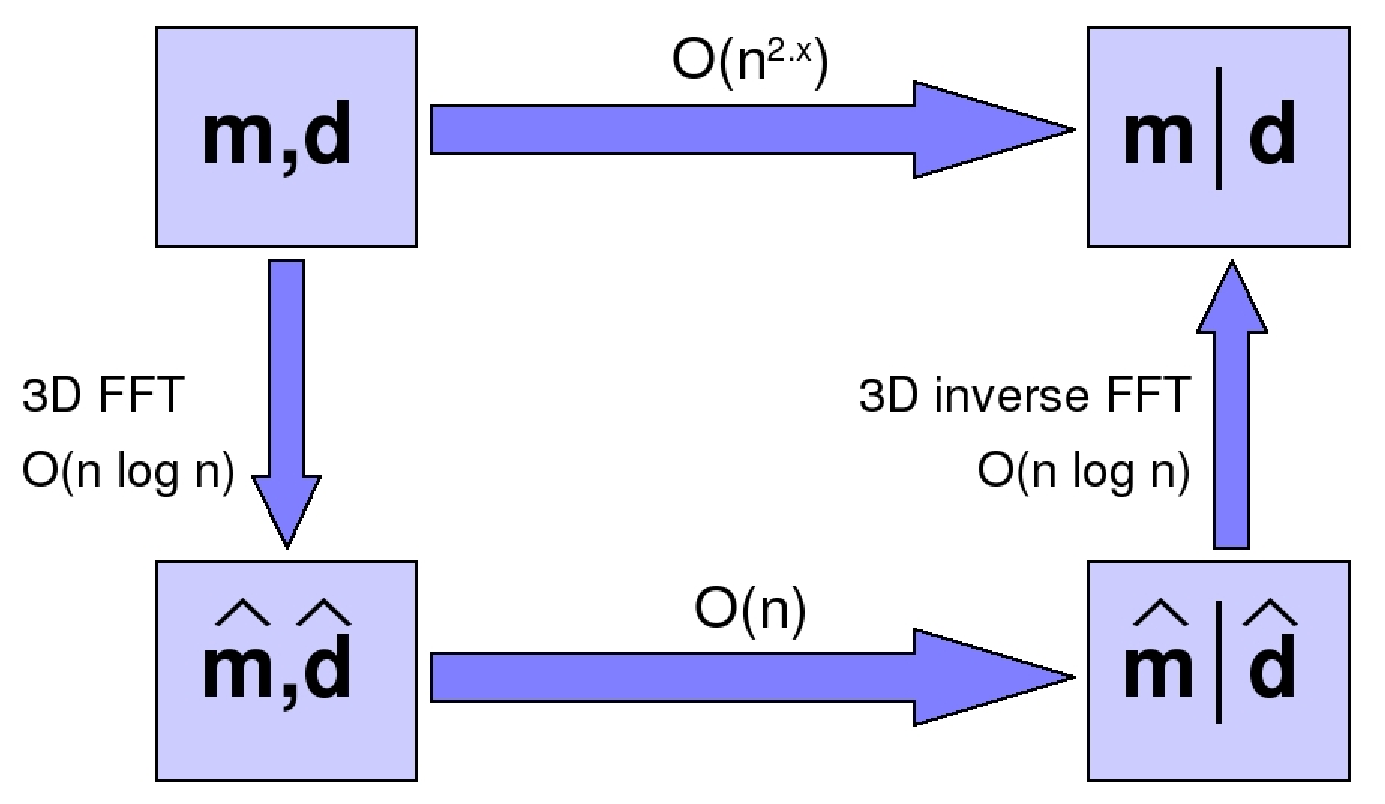
\includegraphics[width=.79\linewidth]{images/FFT_flowdiagram}
  \caption{The problem is transformed to the Fourier domain, solved
  in this domain, and back-transformed to time domain. This reduces
  the problem from a $\mathcal{O}(n^{2.x})$ to a $\mathcal{O}(n\log
  n)$ process.}
  \label{fig:FFT-flowdiagram}
\end{figure}


This seems to require that $\vect{d}$ is stationary, which would imply
that the wavelet must be the same everywhere. However, we can divide
out the wavelet from \autoref{eq:WADm} to obtain 
\begin{equation}
\label{eq:ADm}
\vect{d^\prime} = \vect{A}\vect{D}\vect{m} + \vect{e^\prime},
\end{equation}
where $\vect{d^\prime}$ is the data divided by the wavelet, and
$\vect{e^\prime}$ is the error divided by the wavelet. The details of
how we do this division is given in \autoref{sec:divwavimp}. Note that
we now assume that the noise after division, $\vect{e^\prime}$ is
stationary. Since we assume that a seismic response only depends on
the reflections in that trace, this division can be done trace by
trace. This assumption relies on a rather smooth seismic response, so
the lateral variations in the wavelet should be smooth. We have chosen
to restrict the local wavelet changes to only allow local temporal
shift and amplitude scaling. 

We can also work around the stationary noise assumption, and allow
$\vect{e^\prime}$ to vary laterally. This is done by utilising the
nature of a Bayesian solution, which always is a tradeoff between the
prior and the posterior with noise free data. By finding the posterior
for a minimal noise, we can then interpolate between this solution and
the prior to find an appropriate solution for the local noise
level. When doing this, we ignore the lateral correlation, so we
require constant noise level in each trace, since the conditional
correlations inside a trace are much stronger than between traces. See
\autoref{sec:localnoiseimp} for details. 

\subsection{Facies probabilities}
\label{sec:facprobthe}
To calculate facies probabilities from inverted elastic parameters we
must first establish a link between the elastic parameters from
inversion and facies. There are several ways to do this, and we have
listed the four most realistic in 
\autoref{tab:paramsfacies}.

First, we may establish the link using a rock physics models. This
way we avoid any alignment problems, but we get no frequency control
and get to use no correlation information from the
inversion. A prediction obtained this way tends to be too
optimistic, but if there are no well logs available, this is our only
option.

\begin{table}
\centering
\caption{Different methods for establishing a relation between elastic parameters and facies.}
\label{tab:paramsfacies}
\begin{tabular}{|l|l|l|l|l|l|}
\hline
Approach & Frequency & Inversion   & Alignment & Predictions\\
         & control   & correlation &  & \\ \hline
Rock physics                               &  No &  No & Yes & Optimistic  \\ \hline
Low-pass filtered elastic well logs        & Yes &  No & Yes & Optimistic  \\ \hline
Inversion                                  & Yes & Yes & No  & Pessimistic \\ \hline
Parameter filtered elastic well logs & Yes & Yes & Yes & Realistic   \\ \hline
\end{tabular}
\end{table}

Second, we may filter the elastic well logs using a low-pass filter,
and use these filtered logs and facies logs to make a density
estimation of $p(\bmu_{m|d_{obs}}|f)$, where $f$ is the facies. This
gives us frequency control and proper alignment, but again there are
no correlation information from the inversion included, and the
predictions become to optimistic. The frequency filtering of well logs
is illustrated in \autoref{fig:parmeterfilter}.

\begin{figure}
  \centering
  \fbox{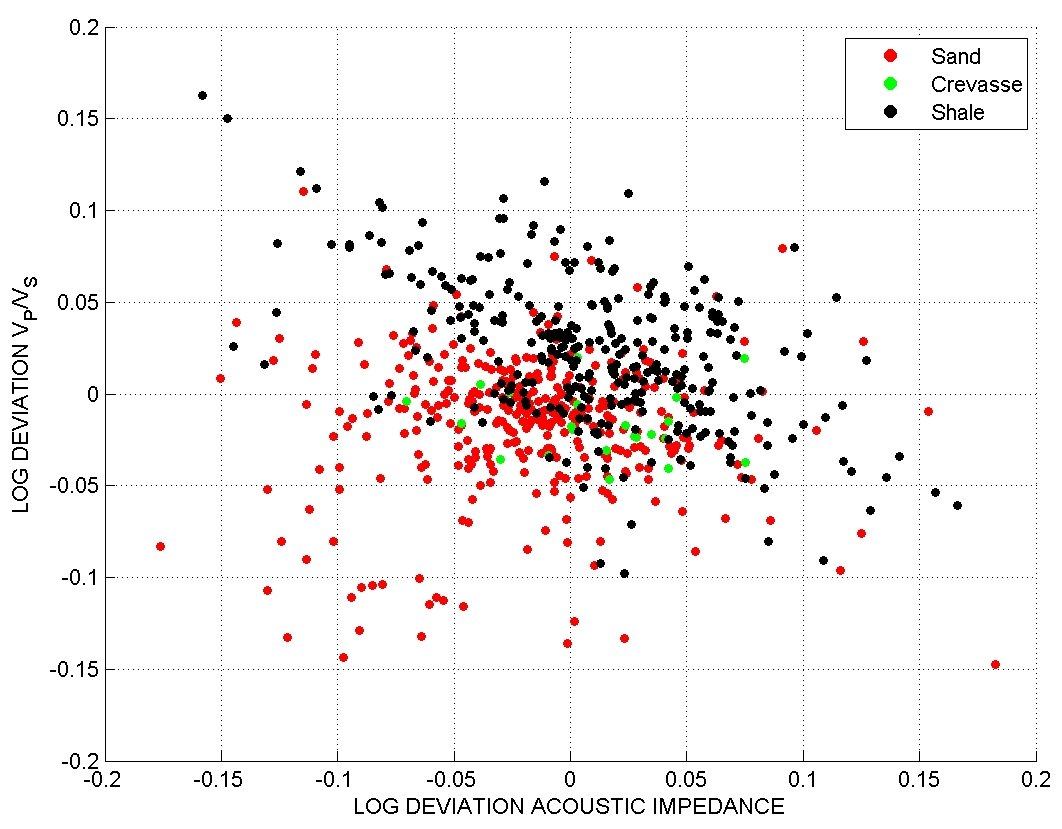
\includegraphics[width=.310\linewidth]{images/Crossplot_raw_logs}}
  \fbox{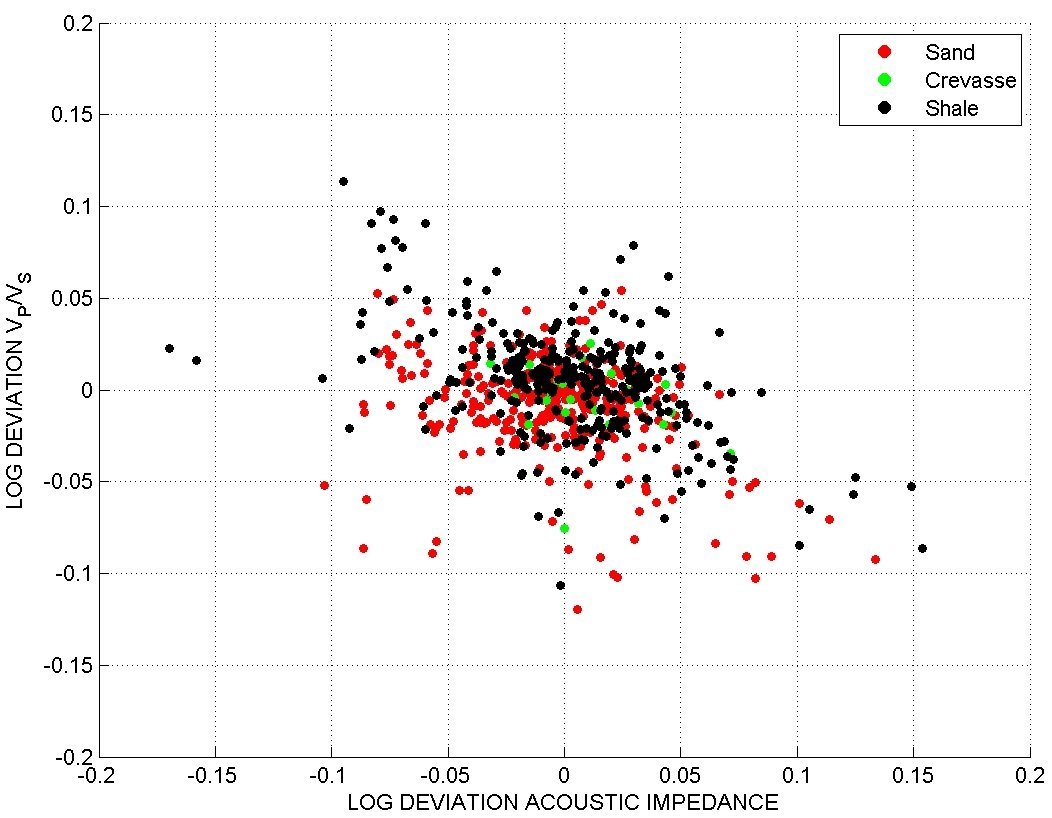
\includegraphics[width=.310\linewidth]{images/Crossplot_40Hz_logs}}
  \fbox{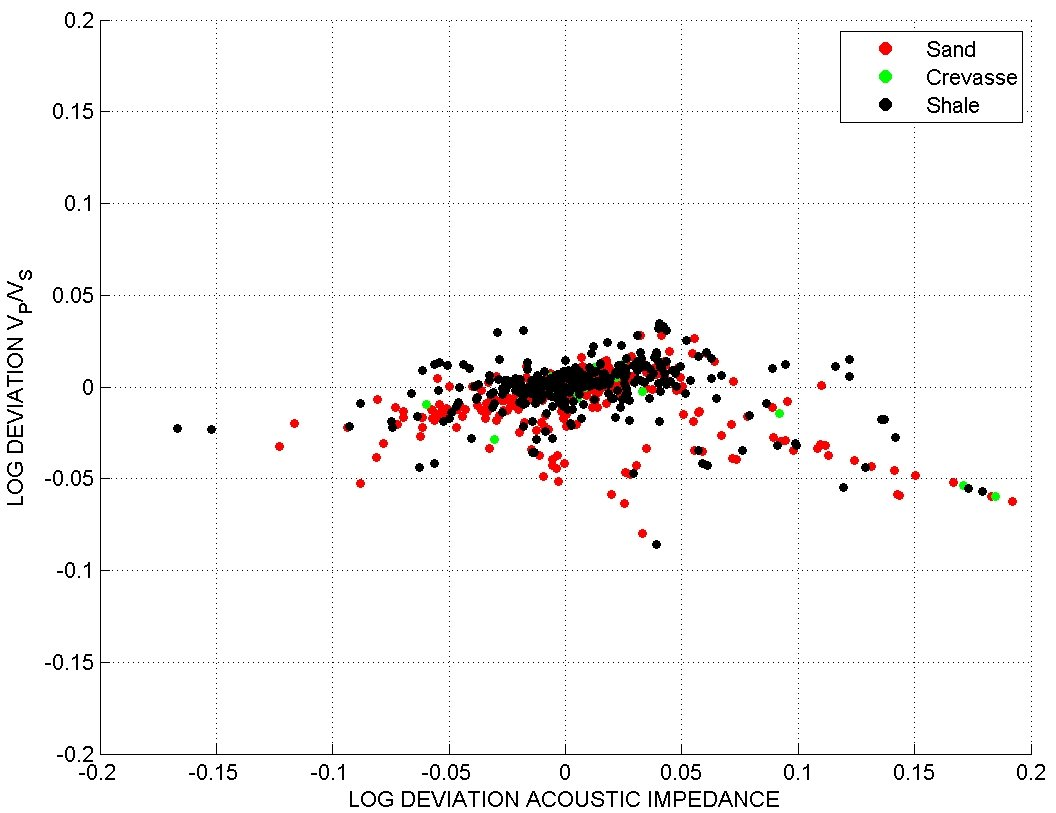
\includegraphics[width=.315\linewidth]{images/Crossplot_multi-parameter_filtered}}
  \caption{Acoustic impedance residuals calculated from blocked raw
    logs plotted against corresponding \vp/\vs  residuals (left), the
    same plot, but with logs high-cut frequency  filtered to 40Hz
    (middle), and the same logs but filtered using frequency and
    correlation information from inversion (right).} 
  \label{fig:parmeterfilter}
\end{figure} 

Third, we may set up the probability density for an elastic responds
given the facies directly from the inverted elastic parameters. This
way we get both frequency control and correlation information
included, but we get no alignment information, and the predictions
become to pessimistic.

Finally, we may establish the density using elastic parameters from
well logs, but filter these using frequency and correlation
information obtained from the inversion. Since we only use well logs
to establish the density estimates, we get no alignment problems, and
in total, this gives us realistic facies predictions. How the
inversion-based filtering differs from the pure frequency-based
filtering mentioned above is illustrated in
\autoref{fig:parmeterfilter}.  

The link between facies and elastic parameters that we eventually are
interested in is $p(f_i|\bmu_{m|d,i})$, where $f_i$ is the facies at
location $i$ and  $\bmu_{m|d,i}$ is the inversion result at the same
location. To establish this link, we must first establish a link
between the well logs $\vect{m}$ and the expectation given the seismic
data $\bmu_{m|d_{obs}}$. We get this 
by combining \autoref{eq:Gm} and 
\autoref{eq:mupost}: 
\begin{eqnarray}
\bmu_{m|d_{obs}} &=&\bmu_{m} +\bSigma_{m}\vect{G}^T \bSigma_{d}^{-1}
                           (\vect{d}_{obs}-\bmu_{d}) \nonumber \\
& = & \bmu_{m} +\bSigma_{m}\vect{G}^T \bSigma_{d}^{-1}
                           (\vect{G}\vect{m}+\vect{e}-\vect{G}\bmu_m) \nonumber\\
& = & \bmu_m + \vect{F}(\vect{m}-\bmu_m)+\vect{e}^*,
\end{eqnarray}
where
\begin{eqnarray}
\vect{F} & = &\bSigma_{m}\vect{G}^T \bSigma_{d}^{-1}\vect{G} \\
\vect{e}^* & \sim & \text{N}(0,\bSigma_{e^*}) \\
\bSigma_{e^*} & = & \bSigma_{m}\vect{G}^T \bSigma_{d}^{-1}\bSigma_e\bSigma_{d}^{-1}\vect{G}\bSigma_m.
\end{eqnarray}
The operator $\vect{F}$ is used to filter the well logs and obtain an
estimate of the expected inversion values $\vect{m}^\ast$. For each
facies, we then do a density estimation of $p(\bmu_{m|d_{obs}}|f)$ for
each possible facies value $f$ using $\vect{m}^\ast$ and facies
logs. The density estimation is done using a kernel smoothing
approach, and by using the distribution of $\vect{e}^*$ as our kernel,
we get an unbiased estimate of this distribution. 

Finally, we find the facies probability:
\begin{equation}
p(f=j|\bmu_{m|d_{obs}}) = \frac{p(\bmu_{m|d_{obs}}|f=j)p(f=j)}{\sum_i p(\bmu_{m|d_{obs}}|f=i)p(f=i)},
\end{equation}
where $p(f=i)$ is the prior probability of facies $i$. This
probability is then computed for each facies and each cell in the
grid, with $\bmu_{m|d_{obs}}$ given by the inversion results.

Far away from wells, the estimates will not be reliable, and we
introduce an undefined facies to show such areas. Denoting the
likelihood of this undefined facies $p(u)$, the facies probabilities
are now calculated as
\begin{equation}
p(f=j|\bmu_{m|d_{obs}}) = \frac{p(\bmu_{m|d_{obs}}|f=j)p(f=j)}{\sum_i p(\bmu_{m|d_{obs}}|f=i)p(f=i)+p(u)},
\end{equation}
where $p(u)$ is uniform over the area, and low compared to the
likelihood for facies when we are close to data. In
Figure~\ref{fig:faciesprobundef} the effect of the undefined facies in
a reservoir consisting of sand and shale is illustrated. The three
figures show cross plots of well observations of $\rho$ against \vp
combined with a probability map shown as a Colo coded map. 

\begin{figure}
  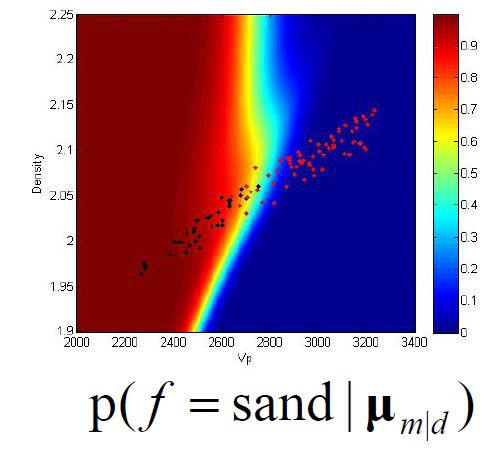
\includegraphics[width=.330\linewidth]{images/faciesprob1}
  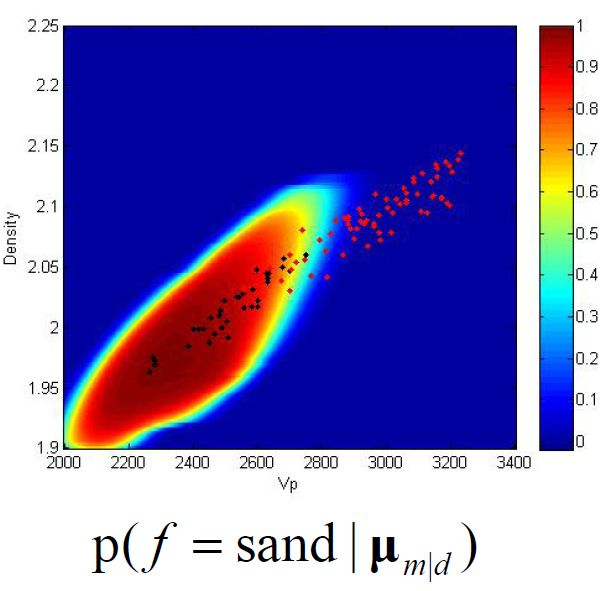
\includegraphics[width=.315\linewidth]{images/faciesprob2}
  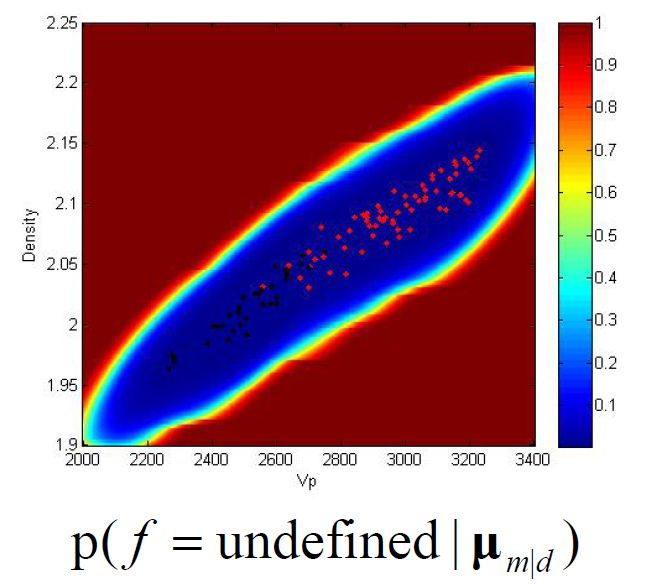
\includegraphics[width=.330\linewidth]{images/faciesprob3}
  \caption{To the left, the posterior sand probability calculated
    without undefined facies. In the middle, the sand probability when
    undefined facies is introduced. To the right, the posterior
    probability for undefined facies.}
  \label{fig:faciesprobundef}
\end{figure} 

In the left figure, we show the probability of sand before the
undefined facies has been introduced. Note how combinations of $\rho$
and \vp which are far away from any well observations, as for instance
(\vp, $\rho$) = (2000m/s, 2.25g/cm$^3$), may still lead to a facies
prediction of sand equal to one. This is not realistic.

In the middle figure, the undefined facies has been introduced, and
whenever we get far away from combinations of $\rho$ and \vp for which
we have no well observations, the probability for sand now decreases
to zero. This does not mean that there is no chance of finding sand at
the current spot, only that we have no data support to tell us what
facies we might find. Similarly, the probability of finding shale will
also be zero.

In the right figure, we show the probability of the undefined
facies. This is zero around well observations, and gradually increases
to one as the distance to observations increase. The probability of
shale may be extracted from these figures since
$p(\text{sand})+p(\text{shale})+p(\text{undefined})=1$.

\newpage
\chapter{Implementation}
\label{sec:implementation}
\index{CRAVA!implementation}

Whereas the general model was explained in \autoref{sec:theory} we
explain a bit more of the actual implementation details here.

The estimation routines implemented in \crava are based on
straightforward and commonly used techniques. This gives fast and
robust estimation, although we may run into problems if the number of
data points is too small, or the data quality is too low. The quality
of an estimation result is never better than the quality of the data
it is based on.

\section{Estimating optimal well location}
The positioning uncertainty between well data and seismic data is
often significant. To overcome this, the well may be moved to the
location with maximum correlation between the seismic data and the
reflection coefficients calculated from the well data. The relation
between the seismic data and reflection coefficients is linear; so
linear covariance is a good measure. The optimal well location is
found by searching for the location with highest covariance in a
lateral neighbourhood around the original well location, where the well
is allowed to be shifted vertically in each target position. The
moving of wells is triggered by a command in the model file, and it is
done prior to the estimation of wavelets, noise, correlations and
background model.

\section{Estimating the prior model}

The prior model for the Bayesian inversion is defined in
equation~\eqref{mdist}, and consists of the expectations of the
elastic parameters $V_p$, $V_s$, and $\rho$ collected in the vector
$\bmu_m$, and their spatial correlation structure collected in the
covariance matrix $\bSigma_m$. These expectations and covariances must
be given prior values before the inversion.

\subsection{Background model}
\index{prior model!background}
\label{sec:backgroundmodel}

The expectation $\bmu_m$ is usually referred to as the background
model. As the seismic data do not contain information about low
frequencies, a background model is built to set the appropriate
levels for the elastic parameters in the inversion volume. To
identify this level, we can plot the frequency content of the seismic
traces in the available wells, and identify lowest frequency for which
seismic data contains enough energy to carry information.

\begin{figure}
\centering
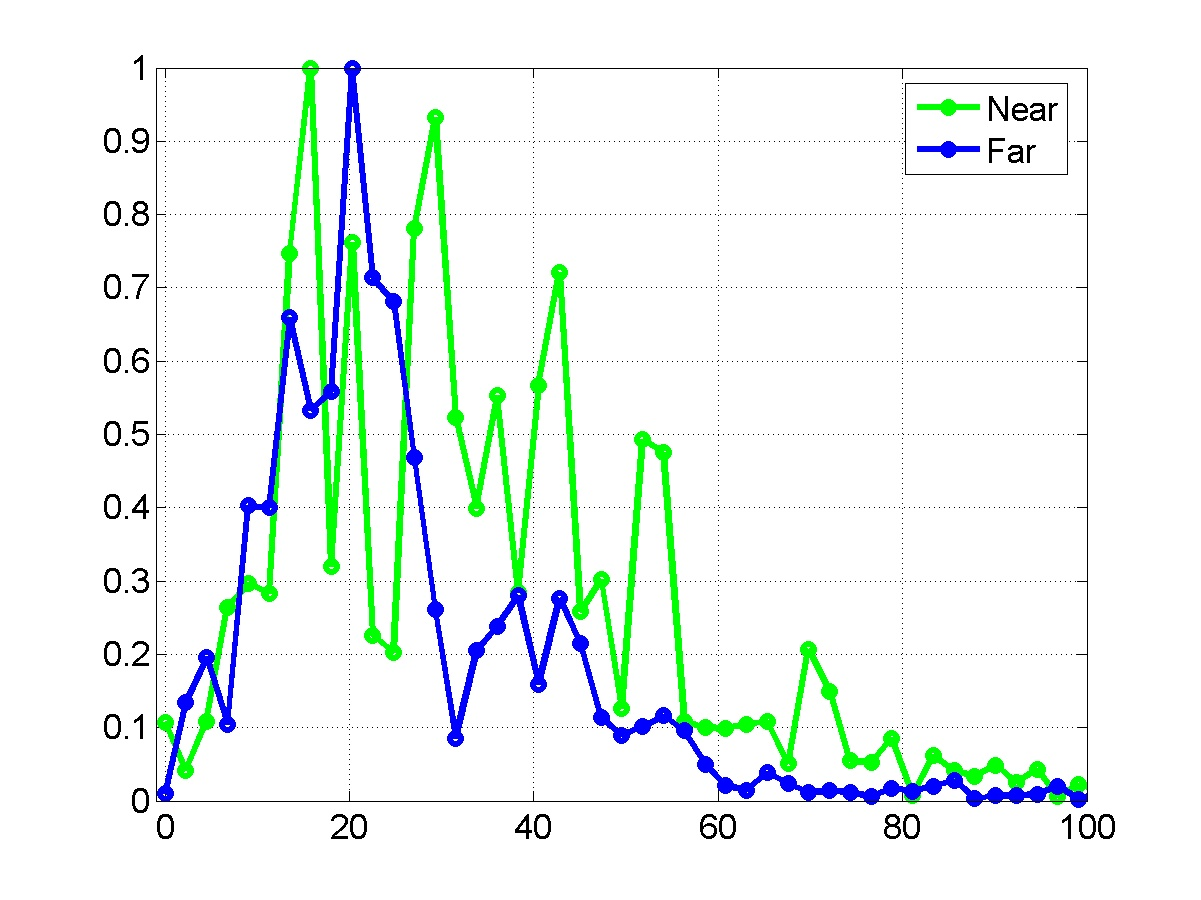
\includegraphics[width=.49\linewidth]{images/implementation/seismicFrequencies_S1}
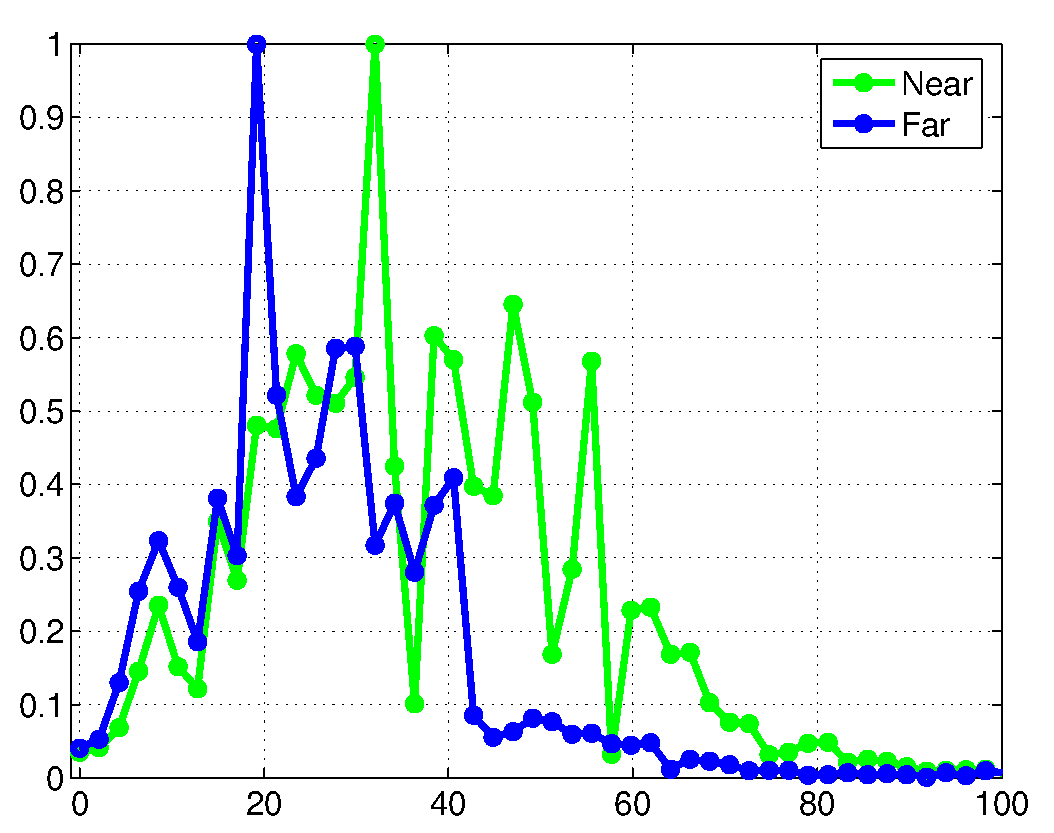
\includegraphics[width=.49\linewidth]{images/implementation/seismicFrequencies_S2}
\caption{The frequency content of the seismic traces in two different
         wells. The frequency content of the near and far stacks are
         shown as green and blue curves respectively.}
\label{fig:frequencycontent}
\end{figure}

In \autoref{fig:frequencycontent}, we have plotted the frequency content
in the seismic data in two different wells. The green curve gives the
frequency content in the near stack and the blue curve gives the
frequency content in the far stack. These plots show that the seismic
data contain little energy below 5--6Hz, and the purpose of the
background model is to fill this void.

The estimation of the background model is made in two steps. First,
we estimate a depth trend for the entire volume, and then we
interpolate well logs into this volume using kriging. The estimation
will by default contain information up to 6Hz, but this high-cut limit
can be adjusted using the \kw{high-cut-background-modelling}
keyword.

When identifying the depth trend, it is important that the wells are
appropriately aligned. The alignment is defined by the time interval
surfaces specified as input, or alternatively, the correlation
direction surface. It is important that the alignment reflects the
correlation structure (deposition/compaction), and if the time
surfaces are either eroding or on-lapped, one should consider specifying
the correlation direction separately using the
\kw{correlation-direction} keyword.

In \autoref{fig:log-aligning}, we show two well logs aligned according
to deposition and according to the true time scale. Evidently, an
incorrect trend will be identified if the true vertical depth is
used. The size of the error will depend on the stratigraphy.

\begin{figure}
\centering
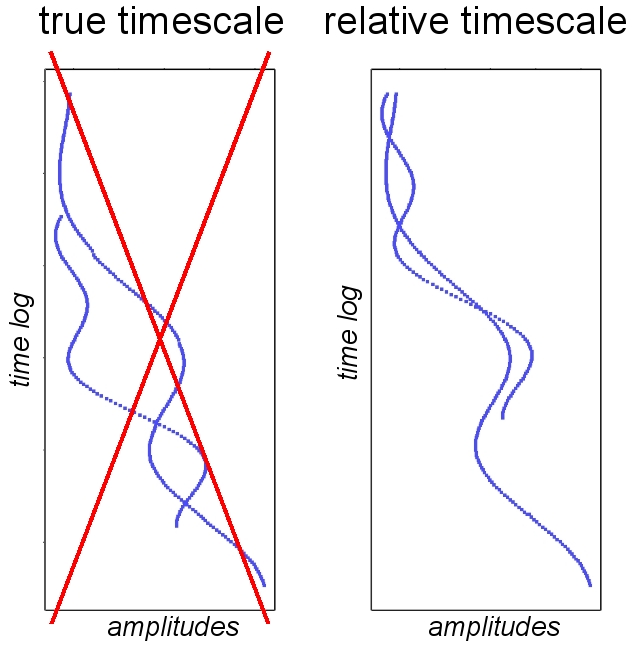
\includegraphics[width=.45\linewidth]{images/implementation/Trend-analysis_dep-vs-comp}
\caption{Well logs aligned according to true time scale (left) and
         according to stratigraphic depth (right).}
\label{fig:log-aligning}
\end{figure}

Assuming properly aligned wells, the trend extraction starts by
calculating an average log value for each layer. This average is
calculated for the \vp, \vs, and $\rho$ well logs and is based on all
available wells. The estimation uses a piecewise linear regression,
rather than the more straightforward arithmetic mean or moving
average, as these measures are sensitive to the amount of data
available. The piecewise regression has the additional advantage
that it can give trend estimates also outside the interval for which
we have data available.

For the linear regression we require a minimum of 10 data points
behind each estimate. In addition, we require that the minimum number
of data points must also be at least 5*N$_\text{wells}$. This way we
ensure that data points from different time samples are always
included. Alternatively, the regression would reduce to an arithmetic
mean whenever there are 10 or more wells available. If we enter a region
with no data points available at all, the minimum requirements are
doubled.

To get the right frequency content in the depth trends, the regression
values are eventually frequency filtered to 6Hz.

The trend extraction process is illustrated in
\autoref{fig:vertical-trends} for the \vp and $\rho$ logs of a field
with six wells. Note that the plots are oriented with layers
as abscissa and log values as ordinate. The blue circles represent log
values from any wells, the green curve is the piecewise linear
regression of these values, and the red curve is the
frequency filtered log that will be used as a depth trend. Note that
the green curve is slightly erratic, especially, as we enter the
region (below reservoir) where there are no data points
available. This shift, which is clearly observed for the density,
arises as we stabilise the estimate by requiring twice as many data
points behind each estimate.

\renewcommand{\floatpagefraction}{0.60}

\begin{figure}
\centering
\fbox{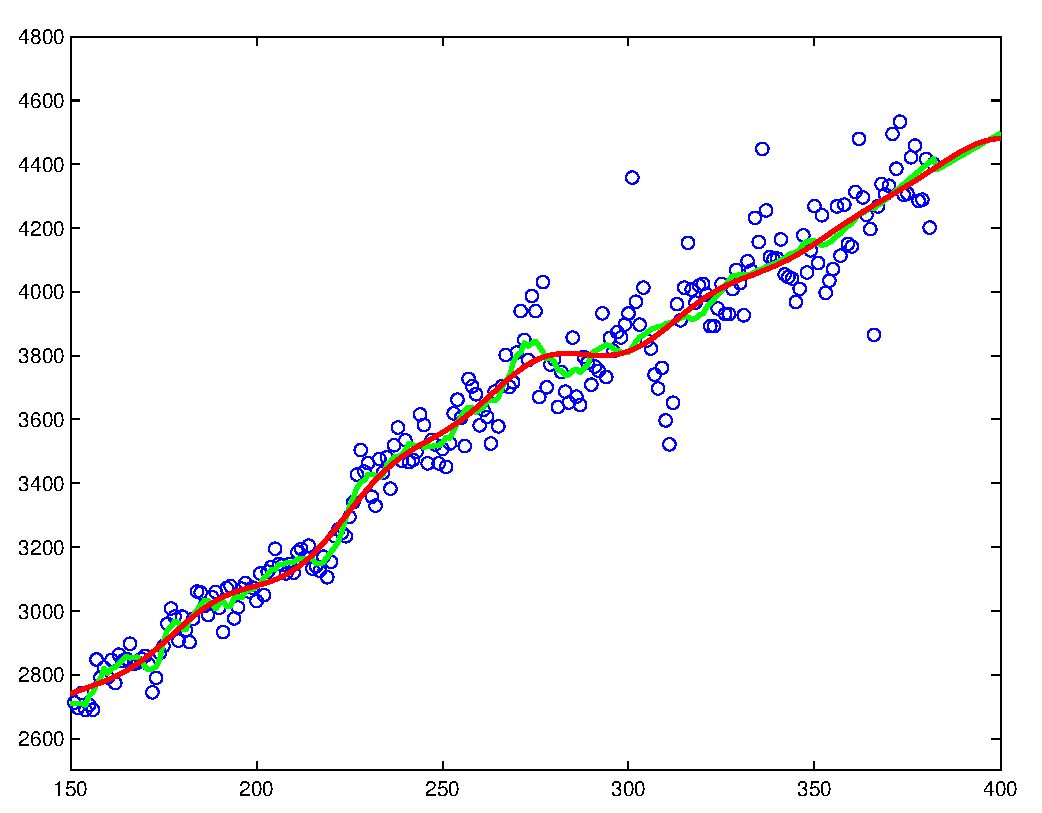
\includegraphics[width=.480\linewidth]{images/implementation/vertical-trend-vp}}
\fbox{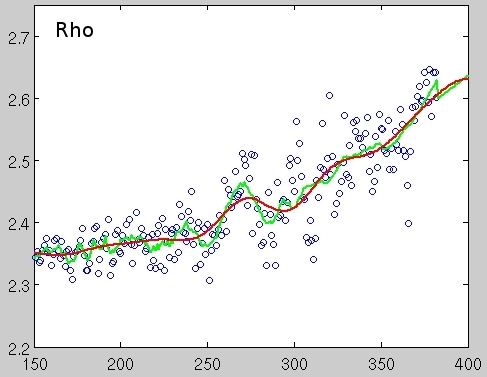
\includegraphics[width=.472\linewidth]{images/implementation/vertical-trend-rho}}
\caption{Well log values plotted against grid layer number for \vp
         (left) and $\rho$ (right). The blue circles show log values,
         the green curve is a piecewise linear regression of the these
         values, and the red curve is the regression values filtered to 6Hz.}
\label{fig:vertical-trends}
%%\end{figure}
%%\begin{figure}
\vspace{1em}
\centering
\fbox{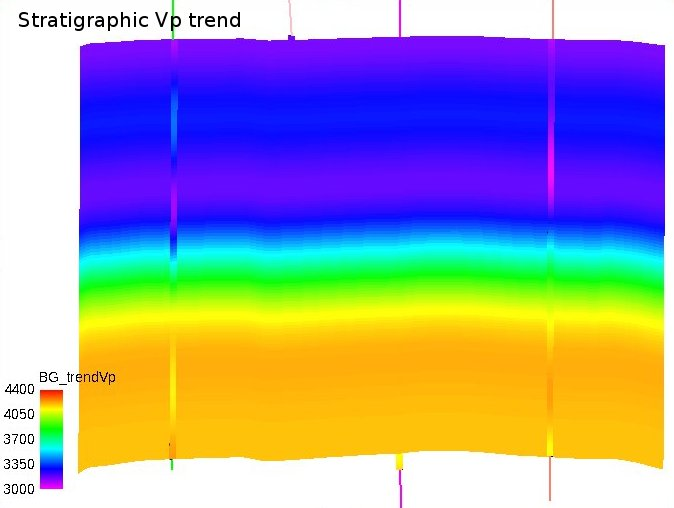
\includegraphics[width=.480\linewidth]{images/implementation/BGtrend_stratigraphic_trend_Vp}}
\fbox{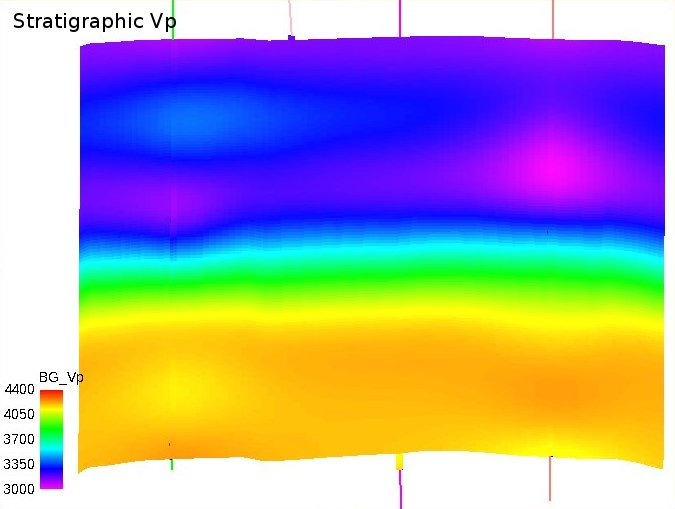
\includegraphics[width=.480\linewidth]{images/implementation/BG_stratigraphic_trend_Vp}}
\caption{\vp depth trend (left) and final background model
  (right). Well logs of \vp, high-cut filtered to 6Hz, are shown for
  comparison.}
\label{fig:background}
\end{figure}

When the inversion volume has been filled with the depth trend, we
interpolate it with 6Hz filtered well logs, to ensure that the
background model will match in wells. A cross section of the resulting
background model for \vp is illustrated in the right part of
\autoref{fig:background}. To the left is the corresponding depth
trend. For comparison the well logs of \vp has plotted in both
illustrations. Note how the wells influence the volume in a region
around the well.

Ideally, the background model should be as smooth as possible,
and a Gaussian variogram model with relatively long ranges may seem an
obvious choice. This model is too smooth, however, and should be
omitted as it often give parameter over- and undershooting away
from wells.

\subsubsection{Multizone background model}
Multizone background model is achieved by doing a \kw{multiple-intervals} inversion and with estimating background models activated. The surfaces are set under \kw{output-volume}. When estimating the multizone background model the reservoir is divided into several horizontal zones defined by surfaces in the inversion volume. In each zone, a local backround model is made by estimating a depth trend for the zone volume, then kriging well logs to the depth trend. The settings for interval uncertainty and erosion priority are set under \kw{multiple-intervals}. The background model in each zone contains frequencies up to 6Hz, but the frequency content is higher in the transitions between the zones. These higher frequencies will, however, contain information about the locations of the zones; hence they contain important prior information. Higher uncertainty gives smoother background models with lower frequency.

\subsubsection{Background model from rock physics}
When rock physics models are used, the background model is generated using these. Each facies is defined as a \kw{rock} possibly containing trends using the rock physics template model described in \autoref{sec:rockPhysics}. The resulting background model is generated as a weighted average of the rock models, where the weights are the corresponding facies \kw{prior-probabilities}. 

If well logs are available, the elastic parameters in the background model, 
i.e.~the expectations, and the corresponding precision/variance, can be 
modelled from data, respectively. Moreover, if there exist appropriate 
reference parameters, like two-way-time and/or stratigraphic depth,
 it is also possible to model the elastic parameters as 1- or 2-dimensional 
functions of the provided reference parameters. 
In principle, these reference parameters can be almost anything, as long as they
provide some underlying structure to the problem at hand.
Also, note that it is possible to combine different models, in the sense that we might 
model the trend as constant while the variance is a two dimensional surface that 
depends on a 2-dimensional reference parameter, see subsection
\ref{sec:assigntrendsrockphy} for more details.

The expectation is fitted using a modified version of a standard 
local linear regression implementation with a Gaussian kernel. In short, what 
distinguishes this implementation from those more commonly used, is that 
it will provide more stable estimates outside the 
main support of data.
This is achieved by gradually increase the bandwidth in the kernel as the method  
extrapolate  away from the main support of the observations. This happens, 
however, at just the right rate to make a smooth transition to a standard linear model
in regions far away from the centre of the observations.
The bandwidth aims at, in all locations, to give a `effective sample sizes', 
i.e.~the total weight of the kernel at a given point, that matches that
in the main support of the data, with a bandwidth set to optimize the asymptotic
properties (limiting minimize mean square error), under the assumption that the 
observations are uniformly distributed over the domain.
 
The estimated variances are a weighted averages between the estimated global variance  
and estimates from a standard implementation of a kernel smoother with a Gaussian 
kernel. The weights, used in the mixture, are the effective sample sizes. The selected 
bandwidth is kept fixed and is the same as used to estimate the expectation 
inside the main support of the data. This construction removes a rather undesirable 
feature of the standard kernel smoother, which estimates a variance that is too low, or 
zero, in regions with few observations.


\subsection{Covariance}
\label{sec:correstimp}

Since we model the covariance structure as separable, we have
collapsed the full time dependent covariances between parameters into
one parameter covariance matrix $\bSigma_{0,m}$, a lateral correlation
vector $\cml(\xi)$, and a temporal correlation vector
$\cmt(\tau)$.

We estimate the correlations by first blocking the wells into the
grid, and then do standard correlation estimation using
\begin{equation}
%%\text{Cov}(X,Y) = \text{E}(XY)-E(X)E(Y),\quad\text{with}\quad
%%X,Y\in\{\ln\vp, \ln\vs, \ln\rho\}
\text{Cov}(X,Y) = \frac{\sum(x_i - \bar{x})(y_j - \bar{y})}{\sqrt{n - 1}},\
  \text{with}\ X,Y\in\{\ln\vp, \ln\vs, \ln\rho\}
\end{equation}

The parameter covariance matrix is simply estimated by using the
covariances at time lag 0. When rock physics models are used, the parameter covariance matrix is calculated from the expectation vector and parameter covariance matrix for each rock model weighted with the corresponding prior facies probability using standard statistical models. If trends are included in the rock physics models, the parameter covariance matrix is calculated in each reservoir position. The resulting parameter covariance matrix is then calculated as the average over these coveraince matrices. 

In \autoref{fig:parameter-correlation}, we
show cross plots of the parameter residuals ($x_i - \bar{x}$) for a
sample field. The depicted distributions look similar to bivariate
normal distributions, which supports the normal distribution
assumptions made in \autoref{mdist}. If there are no \vs logs
available, the prior \vs variance will be set equal to twice the \vp
variance, and their covariance will be set equal to zero.

The temporal correlation is estimated from the remaining lags in the
well logs as depicted in \autoref{fig:temporal-correlation}. The
temporal correlation will be a weighted average of the estimates made
for all three elastic parameters.

While the covariance matrix and the temporal correlation can be readily
estimated from well data, this is not the case for the lateral
correlation, unless there are a large number of wells available. The
lateral correlation is therefore normally chosen parametric. There is
an option in \crava to estimate the lateral correlation from seismic
data, but these estimates are not made relative to stratigraphy and
tend to grossly underestimate the correlation. Using a parametric
correlation function is therefore encouraged. In
\autoref{fig:lateral-correlation}, we have depicted an exponential
correlation function and the lateral correlation structure this kind
of function gives rise to.

\begin{figure}
  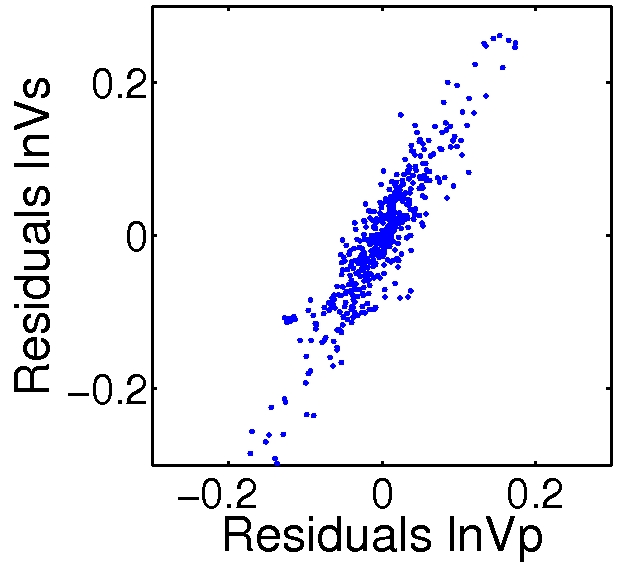
\includegraphics[width=.33\linewidth]{images/implementation/correlation-scatterplot_vp_vs.jpg}
  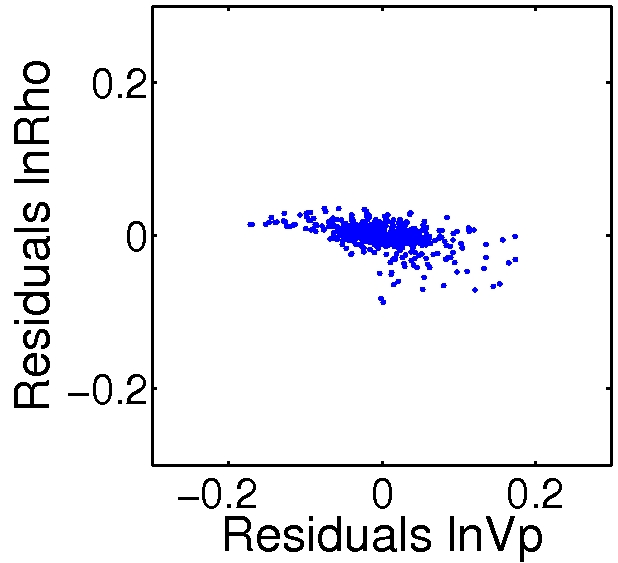
\includegraphics[width=.33\linewidth]{images/implementation/correlation-scatterplot_vp_rho.jpg}
  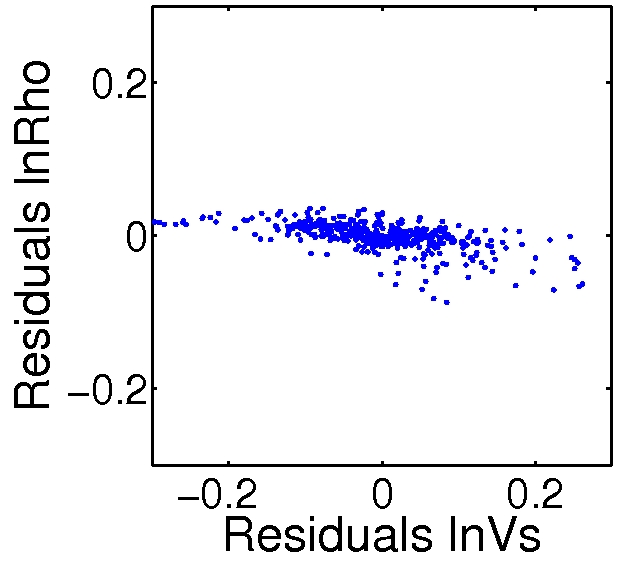
\includegraphics[width=.33\linewidth]{images/implementation/correlation-scatterplot_vs_rho.jpg}
  \caption{Cross plots of logarithmic parameter residuals. From such
           plots the parameter correlations may be estimated.}
  \label{fig:parameter-correlation}
  \vspace{2em}
  \centering
  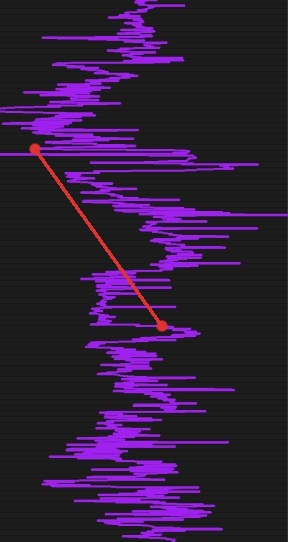
\includegraphics[width=.2\linewidth, height=8.0cm]{images/implementation/temporal_covariance.jpg}\qquad
  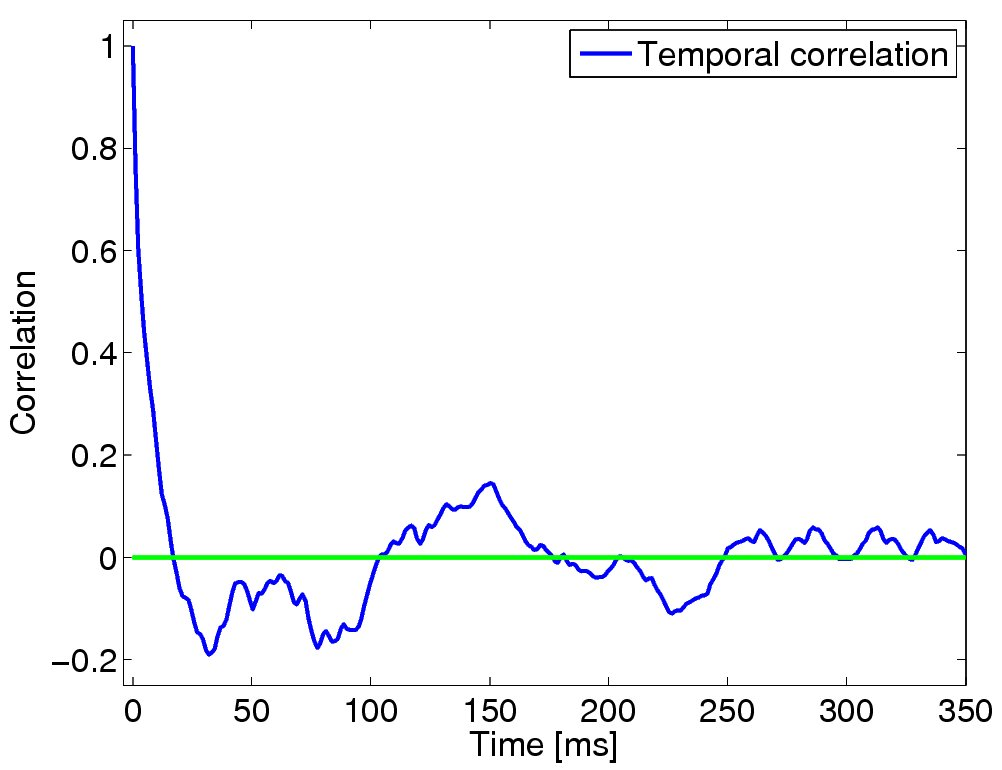
\includegraphics[width=.7\linewidth              ]{images/implementation/temporal_correlation.jpg}
  \caption{We obtain the temporal covariance by measuring the
    covariance between all pairs of points in the well log (left). The
    resulting temporal correlation function (right).}
  \label{fig:temporal-correlation}
  \vspace{2em}
  \centering
  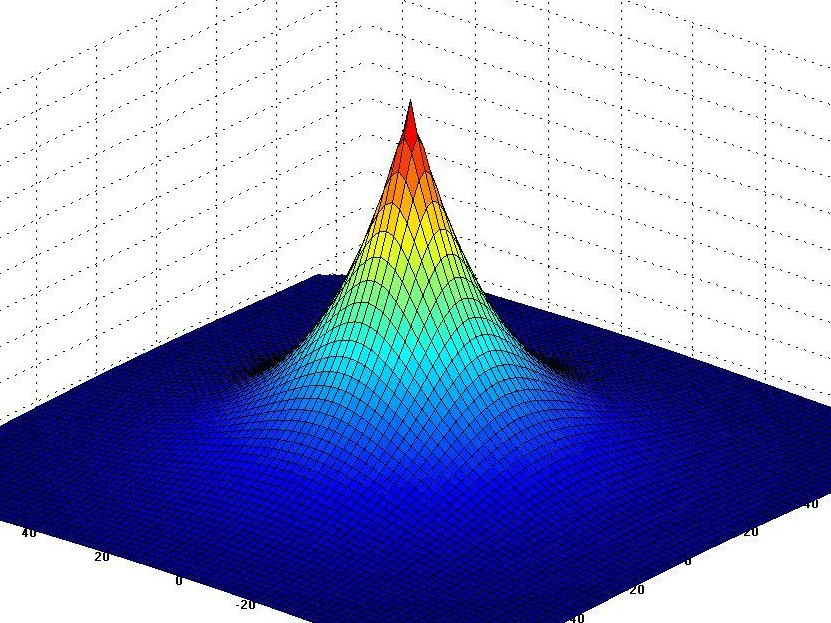
\includegraphics[width=.52\linewidth,height=6cm]{images/implementation/lateral_correlation_1.jpg}\qquad
  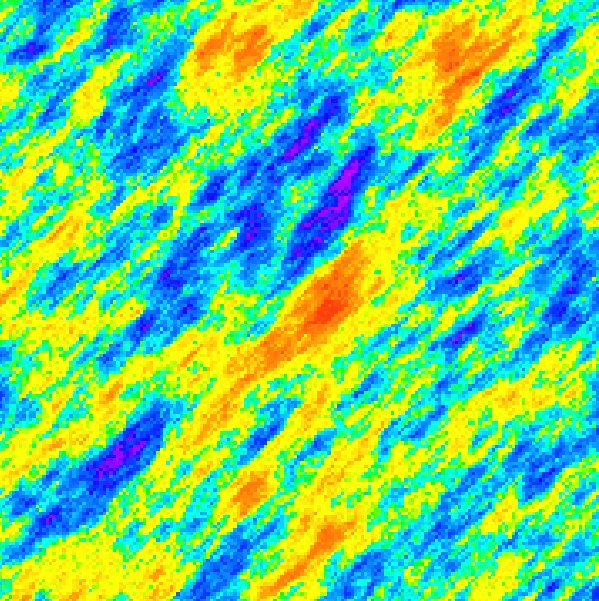
\includegraphics[width=.42\linewidth           ]{images/implementation/lateral_correlation_2.jpg}
  \caption{Parametric lateral correlations. A two-dimensional
    exponential correlation function (left). The lateral correlation
    structure resulting from an anisotropic exponential correlation
    function having an azimuth of $45^\circ$ degrees (right).}
  \label{fig:lateral-correlation}
\end{figure}



\subsection{Likelihood model}

As with the prior model for the elastic parameters, we have also
collapsed the full time dependent error covariance matrix into a noise
covariance matrix $\bSigma_{0,e}$, a lateral correlation vector
$\cel(\xi)$, and a temporal correlation vector $\cet(\tau)$.

The lateral correlation is difficult to estimate and is chosen equal
to that for the elastic parameters, that is, we use $\cel(\xi) =
\cml(\xi)$. The temporal correlation is partly estimated from wavelet
derivatives and partly white noise. By default, a 10\% white noise
fraction is assumed.

For the noise covariance matrix, the noise for a single angle gather
can be either specified in the model file using the
\texttt{<signal-to-noise>} keyword or it can be estimated. A noise
estimate is found by generating synthetic seismic data (see next
section) using the wavelet optimally shifted in each well, and
subtracting this from the seismic data. The remaining part is assumed
to be noise, and we measure the noise energy from this.

The correlation between the noise in different angle stacks is hard to
estimate and is therefore chosen parametric. Typically, an
exponential correlation functions with a range of 10$^\circ$ is
used. In most cases this implies that the noise in the angle stacks
are treated as independent of each other.

\section{Estimating wavelets}
\label{sec:waveestimp}
The implemented wavelet estimation uses the approach of spectral division, see \cite{White84}. 
In this approach an estimate of the cross-correlation between data  
and reflection coefficients, and an estimate of the auto-correlation of reflection coefficients
are used to estimate the wavelet. The methodology requires that the reflection 
coefficients are known,  thus wavelets are estimated at well locations. 
The cross-correlation between data
and reflection coefficients is found by convolving the data with the reflection coefficients, 
and tapering the result. The auto-correlation of the reflection coefficients 
are found similarly by convolving the reflection coefficients with themselves 
and then applying a taper to the result. The tapering is 
performed in order to avoid spurious correlations at large lags.  

Using the standard convolutional relation for seismic data,
\begin{equation}
\vect{d} = \vect{w}*\vect{c}+\vect{e}, \label{fig:syntseis}
\end{equation}
where $\vect{d}$ is the seismic amplitude data, $\vect{w}$ is the
wavelet, $\vect{c}$ the reflection coefficients, and $\vect{e}$ is the
noise. We see that convolving the data with reflection-coefficients, 
transforming to the  Fourier domain, and take the expectation we get
\begin{equation}
d(\omega)\bar{c}(\omega) = w(\omega)|c(\omega)|^2
\end{equation}
Note that the convolution has disappeared, and the equation can be
solved for each frequency $\omega$. We recognise the left hand side as the 
spectre of the cross-correlation between data
and reflection coefficients. And the left hand side as the wavelet multiplied with 
spectre of the auto-correlation of the reflection coefficients. 
This can be obtained by dividing the spectre of the cross-correlation with the 
spectre of the auto-correlation. 

Tapering of the estimated cross-correlation and auto-correlation is required in order to stabilise the estimate. In Crava a Papoulis taper is used. Tapering is equivalent 
to a local smoothing in the frequency domain, thus the resulting wavelet 
estimate will behave smoothly in Fourier domain. 


We find the optimal vertical shift for each well. The global wavelet
is then found by taking the arithmetic average of the zero-phase
wavelets, weighted by the number of samples used from each well.

When using local wavelets, we find the optimal shift and/or scale of
the global wavelet at each well location. Optimal here means
minimising the noise energy. We then use kriging to interpolate this
between wells, with a shift of 0 and a scale of 1 as the mean level
outside the well control area.  This is illustrated in
\autoref{fig:local-wavelet}.

\begin{figure}
  \centering
  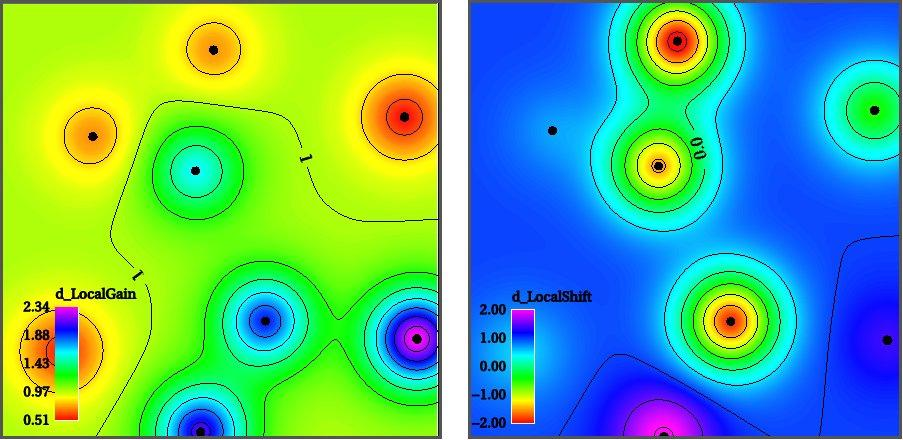
\includegraphics[width=.95\linewidth]{images/local-wavelet}
  \caption{The local scale and shift maps involved when using local wavelets}
  \label{fig:local-wavelet}
\end{figure}

Local noise is estimated using the local noise energies from above. We always use local shift when estimating the noise, but only use local scale if it is used in the inversion. If local scale is used, the noise is divided by this. A noise scaling factor is then computed in each well, and kriged as above.

\section{Estimating 3D wavelet}
\label{sec:3Dwaveestimp}
The expression for the wavenumber representation of the point-spread function given in \autoref{eq:waveletform}
has only one unknown element, namely the 1D pulse $w_0(\omega)$. The functions $\tilde{\alpha}_1$ and $\tilde{H}$ are given as input, together with the average velocity $V_0$. The elements needed for the conversion from depth to time are also input to \crava. That is the reference depth $Z_0$, and reference time surface $T_0$. The theory for the estimation of the 1D pulse is given in \cite{georgsen10}, and with more details in \cite{sand1010}.

As for the 1D wavelet, the pulse is estimated from wells. Using
reflection coefficients from well logs, time gradients estimated from
seismic data around wells and depth gradients computed from time
gradients by using the reference time surface and average velocity given, a matrix $K$ can be constructed forming a linear regression model for the seismic
data as
\begin{equation}
\vect{d} = \vect{K}\vect{w}_0 + \vect{e}.
\end{equation}
The least squares estimate for $\vect{w}_0$ is
\begin{equation}
\widehat{w}_0 = (\vect{K}'\vect{K})^{-1}\vect{G}'\vect{d}.
\end{equation}

\section{Using FFT for inversion}
As previously stated, \autoref{eq:WADm} separates when transformed
into the Fourier domain. After this transformation, the equation
becomes
\begin{equation}
\label{eq:fourierinv}
\vect{\tilde{d}}(\omega,\vect{k}) = \vect{G}(\omega)\vect{\tilde{m}}(\omega,\vect{k}) + \vect{\tilde{e}}(\omega,\vect{k}))
\end{equation}
The tilde denotes the 3D Fourier transform, with temporal
frequency $\omega$, and lateral frequency vector $\vect{k} =
(k_x,k_y)$. Due to the separation, we now have a set of $n$ small
equations, where $n$ is the number of grid cells in the inversion
volume. Everything is still normally distributed, so the solution to
this equation follows the pattern from \autoref{eq:mupost} and
\autoref{eq:sigmapost}. We still must invert a data covariance matrix,
but whereas this matrix had dimension $(n\cdot n_\theta)^2$ before the
Fourier-transform, the matrix we must invert here is reduced to
dimension $n_\theta^2$, where $n_\theta$ is the number of angle
stacks. Since the time for a matrix inversion is almost cubic in size,
it is much faster to invert $n$ of these small matrixes than the one
large. After solving for $\vect{\tilde{m}}(\omega,\vect{k})$, we do
the inverse transform of this to obtain the distribution for
$\vect{m}$. The same does of course hold when we are using local
wavelets that are divided out in advance, \autoref{eq:ADm}. For full
details, see \cite{geo68ab2}.

\section{A note one local wavelet and noise}
\label{sec:nonstationaryimp}
As shown, even though the use of FFT-transform requires stationarity,
we are able to work around this. Wavelets can be made local since
these can be divided out before solving the equations, and locally
higher noise levels can be approximated by interpolating the low-noise
solution and the prior distribution.

\subsection{Local wavelet - dividing out the wavelet}
\label{sec:divwavimp}
A simple division of data by wavelet can easily be done in the Fourier
domain, where the convolution reduces to a multiplication, and the
division can be done one frequency at a time. However, this is very
unstable for frequencies where the wavelet is very weak or not
present, and some sort of stabilisation is needed.

In \crava this is done in two ways. First, we set an upper and lower
cutoff frequency for the wavelet, default set to 5 and 55
Hz. Furthermore, for frequencies that fall below 10\% of the average
amplitude, we set the amplitude to 10\% of average before doing the
division.

\subsection{Local noise}
\label{sec:localnoiseimp}
Local noise is implemented by first finding the solution using the
minimum noise level, to fulfil the stationarity requirements of the
FFT algorithm. We then interpolate the values for each locations
between the prior and this minimum noise posterior. When doing this
interpolation, we ignore correlation between locations. This is not a
problem as long as the noise varies slowly and smoothly.


For each location $\vect{x}$ the adjusted estimate $\tilde{\bmu}_{m|d_{obs}}(\vect{x})$, is found
from the inversion result $\bmu_{m|d_{obs}}(\vect{x})$ by a linear relation,
\begin{equation} \label{eq:LocalAdjustment}
\tilde{\bmu}_{m|d_{obs}}(\vect{x}) = \bmu_{m}(\vect{x}) +\vect{H_x}\left(\bmu_{m|d_{obs}}(\vect{x})-\bmu_{m}(\vect{x})\right),
\end{equation}
The matrix $\vect{H_x}$ is a shrinkage matrix, i.e. the adjusted estimate
is always closer to the prior mean than the inversion result. The matrix
$\vect{H_x}$ depends on the local error variance
 $\bSigma_{e}^x$ and error variance used in the inversion $\bSigma_{e}^0$.

To find the shrinkage matrix we first identify a matrix $\vect{G}_0$
which maps the local prior distribution to the local posterior
distribution when it is observed with the noise $\Sigma_{e}^0$, that is,
$$ \vect{d}(\vect{x}) = \vect{G}_0\vect{m}(\vect{x})+\vect{e}_0,$$
where $\vect{e}_0\sim N\left( \vect{0},\Sigma_{e}^0\right)$.
The inversion of this expression is a linear relation
 \begin{equation} \label{eq:PSigmae}
\bmu_{m|d_{obs}} =\bmu_{m} +\vect{P}(\Sigma_{e}^0)\left(\vect{d}_{obs}-\bmu_{d}\right)
\end{equation}
where  $\vect{P}(\Sigma_{e}^0)=\bSigma_{m}\vect{G}_0^T \left( \vect{G}_0\bSigma_{m}\vect{G_0}^T+\bSigma_{e}^0\right)^{-1}$.

We then define the shrinkage matrix to be:
\begin{equation}\label{eq:H}
\vect{H_x}(\Sigma_{e}^\vect{x},\Sigma_{e}^0) = \vect{P}(\Sigma_{e}^\vect{x})\vect{P}(\Sigma_{e}^0)^{-1}.
\end{equation}
This removes the effect of the standard inversion and add the effect
of the locally adapted inversion. The matrix $\vect{P}(\Sigma_{e}^0)$
is not invertible, but since the local noise always is larger than the
noise in the inversion the product in expression $\ref{eq:H}$ is
always well defined.

\section{Memory handling}
Since the grids needed by \crava can become very large, we try to
keep the number of grids kept simultaneously in memory as small as
possible. This implies that some allocated grids will be used for more
than one purpose. Both padded and unpadded grids are used in \crava,
The amount of memory needed by padded and unpadded grids are
denoted $s_p$ and $s_u$ respectively.
%%The number of padded grids used are counted in detail, while the unpadded grids are
%%only counted in memory computations. In the following, any mention of grid
%%means padded, unpadded will be explicitly stated.

\crava also has an option to use disk space for intermediate storage
of grids. This will reduce the memory consumption with a factor of at
least 2 in realistic cases, but will also increase the computation
time by a factor of almost 3.

\subsection{Grid allocation with all grids in memory}
If intermediate disk storage is not used, the grid memory allocation
will go as follows:

\begin{enumerate}
\item Background grids for Vp, Vs and density, 3 grids.
\item If the background model is to be estimated, another 3 grids are
  allocated for estimation, but destroyed before any other
  allocations.
\item Seismic grids, $n_\theta$. If well optimisation is used, this
  will come before background grids.
\item Possibly prior facies probability grids, indicated by $I_p$,
  $n_f$ unpadded grids.
\item Prior covariance, 6 grids.
\item If relative facies probabilities or local noise, a copy of
  background indicated by $I_b$, 3 grids.
\item {\bf Peak:} At this stage, \crava reaches its first memory
  peak. Minimum memory in use is 10 grids, typical situation with
  three seismic grids and facies modelling requires 15 grids.\\
    Memory usage: $P_1 = (9+n_\theta+I_b*3)*s_p+I_p*n_f*s_u$.
\item The posterior distribution is computed into the background and
  prior covariance grids, and seismic residuals are computed into the
  seismic grids. Thus, the inversion requires no extra grids. (But we
  needed a copy of the background for local noise or facies.)
\item After the inversion, the seismic grids are released, taking us
  off peak down to a base level: \\
  Memory usage:  $P_\text{base} = (9+I_b*3)*s_p+I_p*n_f*s_u$.
\item If simulation is used:
\begin{enumerate}
\item Simulated grids are allocated, 3 grids.
\item If secondary elastic parameters are requested as output (AI,
  $\mu\rho$, etc.), indicated by $I_s$, a computation grid is
  allocated, 1 grid.
\item If kriging is used, indicated by $I_k$, 1 unpadded grid, not
  concurrent with computation grid.
\end{enumerate}
\item {\bf Peak:} New possible peak, since the number of grids now
  allocated may be larger than the released seismic grids. \\
    Memory usage: $P_2 = (12+I_b*3+I_s)*s_p + (I_p*n_f + \max(0,I_k-I_s))*s_u$.
\item New release of grids, back to $P_\text{base}$.
\item If facies probabilities:
\begin{enumerate}
\item 3D histograms of elastic parameters per facies are created, each
  of size 2MB, $n_f$ special grids.
\item Facies probability grids are created, including for undefined,
  $n_f+1$ unpadded grids.
\end{enumerate}
\item {\bf Peak:} New possible peak, since the new memory allocated
  may be larger than the released seismic grids and/or the
  simulation+computation/kriging grids. \\
    Memory usage: $P_3 = (9+I_b*3)*s_p+(I_p*n_f + n_f +1)*s_u + 2*n_f$.
\item Can now release all grids related to facies probability, memory down to $9*s_p$.
\item Eventual kriging of prediction allocates 1 unpadded grid.
\item Everything released.
\end{enumerate}

The maximum memory usage is thus the largest of the actual peaks. The
maximum number of allocated padded grids will occur at either $P_1$ or
$P_2$, whereas the largest number of other grids are allocated at
$P_3$.

\section{Implementation of the rock physics template model}
\label{sec:rf}
The rock physics template model is very flexible, and requires an equally flexible implementation. There are four main elements:
\begin{enumerate}
\item Fluids.
\item Solids.
\item Rocks.
\item Dry-rocks.
\end{enumerate}
We handle these by a dual set of corresponding classes, the distribution classes and the sample classes. We have the set of DistributionFluid, DistributionSolid etc. base classes. These describe the prior distribution for different elements. From these, we can generate samples of the element. These samples are of base classes Fluid, Solid etc., and correspond directly to the Distribution-classes.

Under the base classes, we have a set of derived classes, based on different rock physics models for mixing. These aoos exist on both distribution and sample version. Thus, the tree-like structure of a rock physics template model is mirrored here, with each prior distribution being built as a tree of Distribution... objects, and capable of generating a sample that is a similar tree of sample objects. The sample tree computes it properties as it is built, so the top level knows the resulting elastic parameters.

A feature of the rock physics implementation is that we can update a sample to generate a new sample. This new sample will be highly correlated with the initial sample. This is utilised to generate synthetic well data (for filtering), and when doing 4D modelling. In order to do this updating, each sample stores all the quantiles for the randomly drawn parameters in the sample. When updating a sample, each quantile $u$ is perturbated to a quantile $u_p$ as follows:
\begin{eqnarray}
x = \Phi^{-1}(u) \\
x_p = x + \epsilon \\
u_p = \Phi(x_p).
\end{eqnarray}
Here, $\epsilon$ is normally distributed with expectation 0, and a variance based on the desired correlation. This sampling models the realtion between the existing and new value as a Gaussian pair copula, with a given correlation parameter.

The correlation parameter is controlled in different ways, depending on whether we are generating synthetic wells or setting up a 4D model. In the former case, we use a constant correlation for all random parameters in the sample-tree. This correlation is tuned to obtain the desired correlation between neighbouring samples. In the 4D setting, each random parameter is assigned a yearly correlation (on the distribution level). From this, the correlation for the relevant time step is computed and used for updating. By setting most parameters perfectly correlated, this allows us to update only parameters that are changing in a 4D setting, such as saturation.

\section{Facies probabilities}
How facies probabilities are calculated depends on the input to \crava. If facies probabilities from rock physics is requested, \crava will make synthetic wells from the rock physics models. If rock physics is not used and there are real wells supplied in the input, \crava will make use of these. In both cases, the wells are filtered and used to make a smooth probability distribution from the histogram of observed values. 
\subsection{Trends}
With rock physics, it is also possible to have zero, one or two trends. Trend minimum and maximum values are specified by the user. If the maximum trend value is equal to the minimum value, this is interpreted as having no trend. Each trend axis is divided in 20 bins. Since the grids in general are very large, it is advantageous to keep the number of dimensions low. When there are either one or two trend dimensions, \crava will automatically reduce the three elastic dimensions to the two components that are best resolved by seismic. By minimizing the expression 
\label{eq:geneig}
\begin{equation}
\min_\vect{v} = \frac{\vect{v}^T \vect{\Sigma}_{m|d}\vect{v}}{\vect{v}^T \vect{\Sigma}_{m}\vect{v}}
\end{equation}
once, the best resolved feature is found. The second best feature is found by minimizing the same expression but with the additional constraint of being uncorrelated to the first component. This amounts to choosing the eigenvectors of $\vect{\Sigma}_{m}^{-1}\vect{\Sigma}_{m|d}$ sorted in increasing order of the corresponding eigenvalues. However, the use of trends will increase the number of numerical grids in use in \crava :
\begin{enumerate}
\item With real wells and no rock physics: the wells are filtered and a 3D grid (where the three dimensions represent the three elastic parameters) is filled with the observed values.
\item If facies probabilites from rock physics is requested:
\begin{enumerate}
\item With no trend, a 3D grid is filled with values from the synthetic wells. 
\item With one trend, the three elastic dimensions are reduced to two dimensions and 20 (the number of bins in the trend dimension) 2D grids (actually 3D grids where only two dimensions are in use) are filled.
\item With two trends, the three elastic dimensions are reduced to two dimensions and $20^2=4000$ (the number of bins in the trend dimension) 2D grids (actually 3D grids where only two dimensions are in use) are filled.
\end{enumerate}
\end{enumerate}

\subsection{Synthetic wells}
When rock physics is used, 10 synthetic wells, each of minimum length 100 bins, is simulated per combination of trend parameters. If no trends are used, 10 such wells are simulated. The synthetic wells are made as follows:
\begin{enumerate}
\item If the length of the well is less than 100 bins, draw one of the relevant facies from a uniform distribution (no correlation with the facies above).
\item Draw a facies length from a geometric distribution with expectation 10 ms.
\item Generate a well sample of this length by calling the functionality described in section~\ref{sec:rf} and add this piece to the well.
\end{enumerate}

\subsection{Well filtering and smoothing}
The final probability distribution is smoothed with the seismic uncertainty. This uncertainty is calculated using the prior and posterior spatial covariance for the elastic parameters in the well. For both real and synthetic wells, the distribution of the error in the inversion is calculated as
\label{eq:}
\begin{equation}
\vect{\Sigma}_{e^*,w} = \vect{\Sigma}_{m,w|d} - \vect{\Sigma}_{m,w|d} \vect{\Sigma}_{m,w}^{-1} \vect{\Sigma}_{m,w|d}
\end{equation}
Each well is filtered independently. The bins in the probability grids (one per facies) are then filled with the values from the wells and a Gaussian distribution with covariance in the elastic dimensions from the well filter is created. The facies probability grids are then convoluted with the Gaussian distribution by FFT. This gives $ \hat{p}(\hat{\vect{m}}_i|f_i,\vect{z}) $.
\subsection{Calculating facies probabilities}
The final lithology prediction is computed as
\begin{equation}
\hat{p}(f_i|\hat{m}_i,z) = \frac{\hat{p}(\hat{\vect{m}}_i|f_i,\vect{z}) p(f_i|\vect{z})}{\Sigma_{f_i} \hat{p}(\hat{\vect{m}}_i|f_i,\vect{z}) p(f_i|\vect{z})}
\end{equation} 
The \kw{uncertainty-level} is part of the input to \crava and specifies the likelihood for undefined lithologies. This value is scaled according to the size of the grid, but will result in a high probability for undefined facies if the relevant point is not close to one of the modes in the distribution.

\newpage
\chapter{User guide}
\label{sec:userguide}
\index{CRAVA!userguide}

In this chapter, we describe how to build a \crava model file. The
model file mainly follows the XML format, but we also use the
character '\#' for commenting, meaning that the rest of the line after
such a character is read as comment. XML files are built with start
and end tags, encapsulating either tags or values. All model files start
with \texttt{<crava>}, and end with \texttt{</crava>}. An example of a
model file is given in \autoref{sec:crava-model-file}. 

\section{Basic inversion}
\label{sec:basicinv}
\index{inversion!basic}
A primary ability for \crava is to run simple first-pass
inversions. In this section, we describe how to build a model file for
a simple inversion. We focus on how to get the key information into
the program, whereas more detailed controls are discussed later, in
\autoref{sec:advinvusr}. The key information elements for a \crava
inversion run is: 
\begin{itemize}
\item \hyperref[sec:basicseis]{Seismic data}.
\item \hyperref[sec:basicwave]{Wavelet}.
\item \hyperref[sec:basicnoise]{Signal/noise ratio}.
\item \hyperref[sec:basicvol]{Inversion volume}.
\item \hyperref[sec:basicbg]{Background model}.
\item \hyperref[sec:basiccorr]{Correlation structures}.
\end{itemize}
Since \crava is designed to estimate any information that is not
given, well data must also commonly be included. 

\subsection{Survey information}
All information regarding the seismic data is gathered under the
\kw{survey}\kwindex{survey} tag. This includes the file names for
seismic data files, wavelet information and signal-to-noise ratio for
each angle gather. As an example, it may look like this: 
\svex{ex:survey}
<crava>
<survey>
  <segy-start-time>             2500.0 </segy-start-time>
  <angle-gather>
    <offset-angle>                16.0 </offset-angle>
    <seismic-data>
      <file-name>  seismic/Cube16.segy </file-name>
    </seismic-data>
  </angle-gather>
  <angle-gather>
    <offset-angle>                28.0 </offset-angle>
    <seismic-data>
      <file-name>  seismic/Cube28.segy </file-name>
    </seismic-data>
  </angle-gather>
</survey>
</crava>
\end{verbatim}
\end{example}

The seismic data can be given on SegY-format, with a common offset time
specified by the keyword \kw{segy-start-time}\kwindex{segy-start-time}
if the offset is different from 0. The first value is used to
represent the interval from start-time to start-time + time-step, so
with a start-time of 100ms, and 4ms sampling, the first value is used
in the grid cell covering the interval 100-104ms. If we use seismic
data of another format than SegY, the \kw{segy-start-time} command is
not used. The file format is detected automatically by \crava.

For each available angle, the rest of the information is gathered under an \kw{angle-gather} tag, one for each offset. The actual angle is given by \kw{offset-angle}\kwindex{offset-angle}.

\subsubsection{Seismic data}
\label{sec:basicseis}
The name of the seismic data file is given with \kw{file-name}, as seen in \autoref{ex:survey}. Naturally, seismic data is always required when running an inversion.
By default, \crava recognises four SegY formats; Seisworks, Charisma, SIP and IESX, see Table~\ref{tab:segyformats}. 
\begin{table}[h]
\centering
\caption{SegY formats recognised by Crava}
\label{tab:segyformats}
\begin{tabular}{|l|r|r|r|r|r|r|c|}
\hline
Name & X & Y & IL & XL & Offset & CoordScal & CoordSys \\ \hline \hline
SeisWorks & 73 & 77 & 9 & 21 & 109 & 71 & UTM \\ \hline
Charisma & 73 & 77 & 5 & 21 & 109 & 71 & UTM \\ \hline
IESX & 73 & 77 & 221 & 21 & 109 & 71 & UTM \\ \hline
SIP & 181 & 185 & 189 & 193 & 37 & 71 & UTM  \\ \hline
\end{tabular}
\end{table}

You are also allowed to define your own format using the \kw{segy-format}\kwindex{segy-format} command. A standard format is given by \kw{standard-format}. Possible arguments are 'seisworks', 'iesx', 'charisma' or 'SIP'. Modifications to the chosen standard format can be given by the following commands: \kw{location-x}, \kw{location-y}, \kw{location-il}, \kw{location-xl}, \kw{location-offset} and \kw{bypass-coordinate-scaling}. For more information on how to use this, see \kw{segy-format} in the reference manual chapter.
 
Other file formats recognised by \crava are storm, Sgri and crava.

\subsubsection{Wavelet}
\label{sec:basicwave}
To invert the seismic data, we need a wavelet for each angle. This wavelet can be read from file, using the \kw{wavelet}\kwindex{wavelet} and \rkw{file-name}{file-name2} commands like this:
\svex{ex:wavelet}
  <angle-gather>
    <offset-angle>     16.0 </offset-angle>
    <seismic-data>
      <file-name>  seismic/Cube16.segy </file-name>
    </seismic-data>
    <wavelet>
      <file-name>  wavelets/wavelet16.txt </file-name>
    </wavelet>
  </angle-gather>
\end{verbatim}
\end{example}

We can read wavelets on JASON and NORSAR format.

The Ricker wavelet is implemented in \crava, and can be used by the command \kw{ricker}\kwindex{ricker}. The peak frequency is given as argument.

If the \kw{wavelet} command is not given, or given without \kw{file-name}, the wavelet is estimated. See \autoref{sec:waveestimp} for how this is done. If the wavelet is given on file, but not scaled, the command \kw{scale}\kwindex{scale} should be used if the scale is known, otherwise, the scale can be estimated by using the \kw{estimate-scale}\kwindex{estimate-scale} command. If none of these are specified, the wavelet will be used as it is on file.

\subsubsection{Signal/noise ratio}
\label{sec:basicnoise}
This ratio is given with \kw{signal-to-noise-ratio}\kwindex{signal-to-noise-ratio}. If this command is not given, the ratio is estimated. Note that we define the signal to noise ratio as the data variance divided by the error variance, where the data variance is model variance plus error variance.

\subsection{Inversion volume}
\label{sec:basicvol}
The volume used for inversion is given horizontally by a rectangle, and vertically bounded by a top and base surface. It is defined by the command \kw{output-volume}\kwindex{output-volume} under \kw{project-settings}. It is possible to perform either single or multiple interval inversion.

\subsubsection{Single interval inversion}
The output volume for single interval inversion is set by one top and one base surface by the keyword \kw{interval-two-surfaces} or \kw{interval-one-surface} where a top surface and thickness are given.  Typically, it may look something like this:
\svex{ex:volume}
<crava>
<project-settings>
  <output-volume>
    <utm-coordinates>
      <reference-point-x>  403050.0   </reference-point-x>
      <reference-point-y> 7211900.0   </reference-point-y>
      <length-x>              500.0   </length-x>
      <length-y>              500.0   </length-y>
      <angle>                  23.627 </angle>
      <sample-density-x>       50.0   </sample-density-x>
      <sample-density-y>       50.0   </sample-density-y>
    </utm-coordinates>

    <interval-two-surfaces>
      <top-surface>
        <time-file>   horizons/FlatTop_3100ms.storm </time-file>
      </top-surface>
      <base-surface>
        <time-file>   horizons/FlatBase_3600ms.storm </time-file>
      </base-surface>
      <number-of-layers> 125 </number-of-layers>
    </interval-two-surfaces>
  </output-volume>
</project-settings>
</crava>
\end{verbatim}
\end{example}

\subsubsection{Multiple interval inversion}
To perform multiple interval inversion one must define several surfaces in the \kw{multiple-intervals}. Here one defines one top surface and several base surfaces (one for each interval). In addition one must set the \kw{erosion-priority} which defines which surface to be used when two surfaces intersect. All the base surfaces need to be given a unique priority. The surface with highest priority is given erosion priority two (top surface has priority one), while the surface with lowest priority is given priority n, where n is equal to the number of surfaces.

The inversion is done separately for each interval and finally combined to a final grid, which consist of the first top surface and the last base surface. The resolution used in the output grid is taken from the smallest resolution from all intervals. One can also set the \kw{uncertainty} for all base surfaces, this is used to smooth results across border when they are merged to a final grid. To represent uncertainties between intervals a beta distribution with parameters $\alpha = \beta = 2$ is used. The distribution is symmetric around its center, being the surface between the intervals. The limits in the Beta distribution, given by the keyword \kw{uncertainty}, is the distance of the uncertainty in ms in each direction from the surface. 

Each interval given in \kw{multiple-intervals} are defined by a name. This name is used as a reference when other interval based settings are set. These are \kw{vp-vs-ratio}, \kw{correlation-direction}, \kw{parameter-autocovariance}, \kw{prior-probabilities} and \kw{volume-fractions}.

It may look something like this:
\svex{ex:volume-multiple}
<crava>
<project-settings>
  <output-volume>
    <utm-coordinates>
      <reference-point-x>  403050.0   </reference-point-x>
      <reference-point-y> 7211900.0   </reference-point-y>
      <length-x>              500.0   </length-x>
      <length-y>              500.0   </length-y>
      <angle>                  23.627 </angle>
      <sample-density-x>       50.0   </sample-density-x>
      <sample-density-y>       50.0   </sample-density-y>
    </utm-coordinates>

    <multiple-intervals>
      <top-surface>
        <time-file>   horizons/FlatTop_3100ms.storm </time-file>
      </top-surface>
      <interval>
        <name>IntervalA</name>
        <base-surface>
      	  <time-file>horizons/BaseA.storm</time-file>
      	  <erosion-priority>2</erosion-priority>
          <uncertainty>60</uncertainty>
    	</base-surface>
    	<number-of-layers>100</number-of-layers>
      </interval>
      <interval>
    	<name>IntervalB</name>
        <base-surface>
      	  <time-file>horizons/BaseB.storm</time-file>
      	  <erosion-priority>4</erosion-priority>
          <uncertainty>40</uncertainty>
    	</base-surface>
    	<number-of-layers>120</number-of-layers>
	  </interval> 
    </multiple-intervals>
  </output-volume>
</project-settings>
</crava>
\end{verbatim}
\end{example}


\subsubsection{Lateral extent}
The lateral extent of the inversion volume is specified by the command
\kw{area-from-surface}\kwindex{area-from-surface},
\kw{utm-coordinates}\kwindex{utm-coordinates}, or
\kw{inline-crossline-numbers}\kwindex{inline-crossline-numbers}. The 
command \kw{utm-coordinates} describes a rectangle, which may be
rotated relative to the seismic data. It has the following parameters,
which must all be specified: 
\begin{itemize}
\item \kw{reference-point-x}\kwindex{reference-point-x} is the UTM x-coordinate of one corner of the area.
\item \kw{reference-point-y}\kwindex{reference-point-y} is the UTM y-coordinate of the same corner.
\item \kw{length-x}\kwindex{length-x} is the extent of the area along the local x-axis.
\item \kw{length-y}\kwindex{length-y} is the extent of the area along the local y-axis.
\item \kw{angle}\kwindex{angle} is the angle between the direction of the UTM x-axis and the local x-axis. Positive angles are counterclockwise.
\item \kw{sample-density-x}\kwindex{sample-density-x} is the length of one grid cell along the local x-axis.
\item \kw{sample-density-y}\kwindex{sample-density-y} is the length of one grid cell along the local y-axis.
\end{itemize}
If the grid has the same rotation as the SegY volume read as input, output SegY volumes will have correct in-lines and cross-lines. Otherwise, these numbers are just counting from the initial corner.
The command \kw{area-from-surface} contains only one parameter, \kw{file-name}\kwindex{file-name}, the name of a storm surface file defining the lateral extent of the inversion volume.
The last way to define the inversion area is by the command \kw{inline-crossline-numbers}\kwindex{inline-crossline-numbers}. By this command, the following parameters can be used:
\begin{itemize}
\item \kw{il-start}\kwindex{il-start} is the starting inline number.
\item \kw{il-end}\kwindex{il-end} is the ending inline number.
\item \kw{xl-start}\kwindex{xl-start} is the starting crossline number.
\item \kw{xl-end}\kwindex{xl-end} is the ending crossline number.
\item \kw{il-step}\kwindex{il-step} is the inline interval.
\item \kw{xl-step}\kwindex{xl-step} is the crossline interval.
\end{itemize}
The parameters \kw{il-start} and \kw{xl-start} must be set if this command is used, the other parameters are optional. If they are not given, the numbers are taken from the Segy file containing the first seismic cube.

The area commands may be skipped altogether. The area will then be taken from the first input seismic data file, and defined as the smallest rectangle that covers all traces.

\subsubsection{Top and base surfaces}
The vertical extent is normally given by a top and a base surface in
time, under the command \kw{interval-two-surfaces}
\kwindex{interval-two-surfaces}, as shown in \autoref{ex:volume}. The
file name for the top surface is given under command
\kw{top-surface}\kwindex{top-surface}, \kw{time-file}, and the base
surface is given similarly under \kw{base-surface}
\kwindex{base-surface}, \kw{time-file}. The file format is binary
storm, ASCII Irap, Multicolumn ASCII format (file with five columns,
x, y, z, IL and XL) or XYZ ASCII (file with three columns, x, y z). The last two surfaces must follow the segy geometry. Top and base time values for the inversion
interval can be given as constants instead of files, by using the
command \kw{time-value}\kwindex{time-value}.   

These surfaces also define the default lateral correlation direction
for the elastic parameters, with the correlation being parallel to the
top surface at the top, and base surface at the base. Between this, we
create a top- and base-conform grid, so that the number of grid cells
in each trace is constant, although the interval thickness may
vary. This is shown in part B of
\autoref{fig:inversion-interval-types}. The inversion may be unstable
if the resolution varies too much in different traces, so we recommend
that no trace interval is larger than twice the shortest interval. The
number of layers between top and base is given by the command
\kw{number-of-layers} \kwindex{number-of-layers}.

%\begin{figure}
%  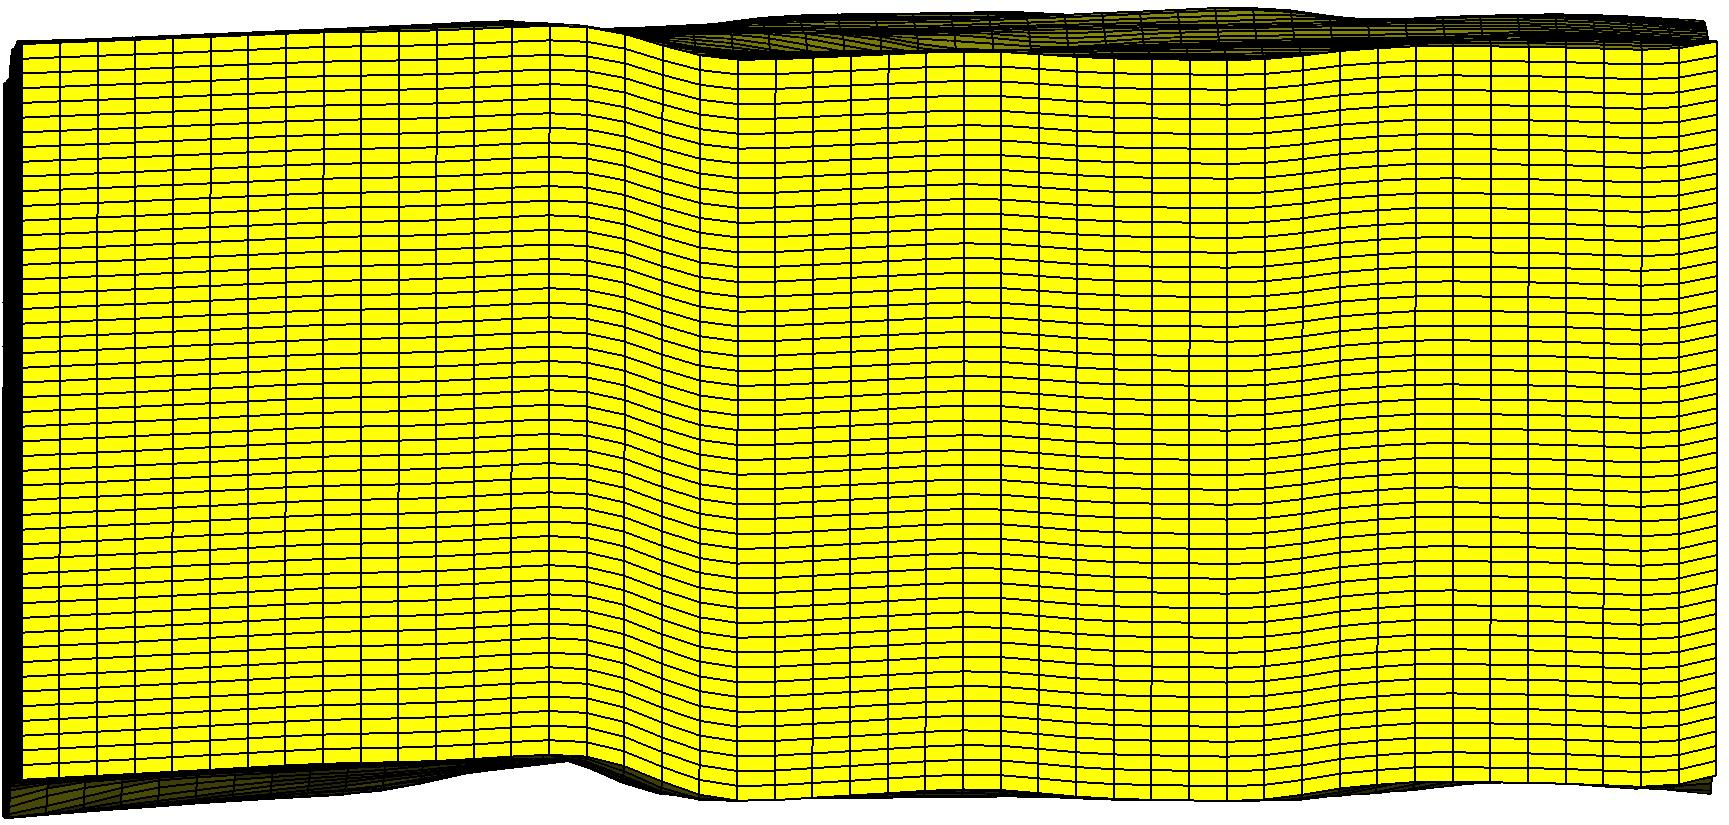
\includegraphics[width=.99\linewidth]{images/conformgrid}
%  \caption{The layer structure of a top- and base-conform grid.}
%  \label{fig:conformgrid}
%\end{figure}

\begin{figure}
  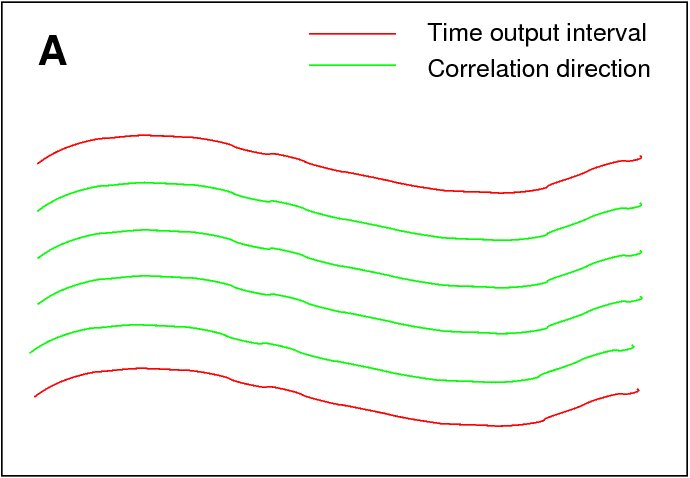
\includegraphics[width=.49\linewidth]{images/A_correlation_parallel}
  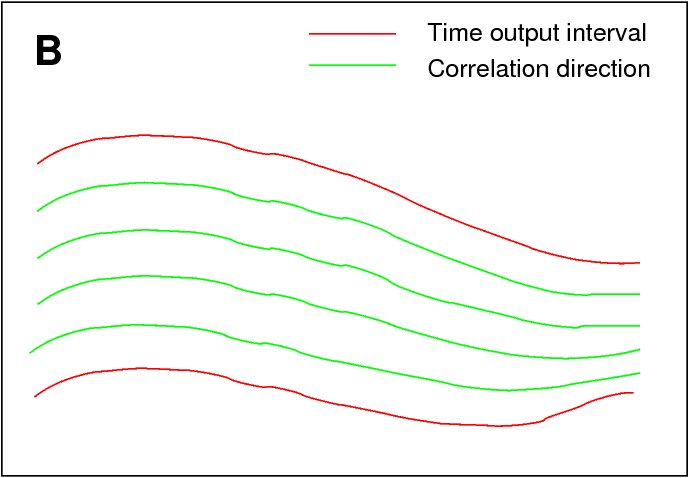
\includegraphics[width=.49\linewidth]{images/B_correlation_proportional}\\
  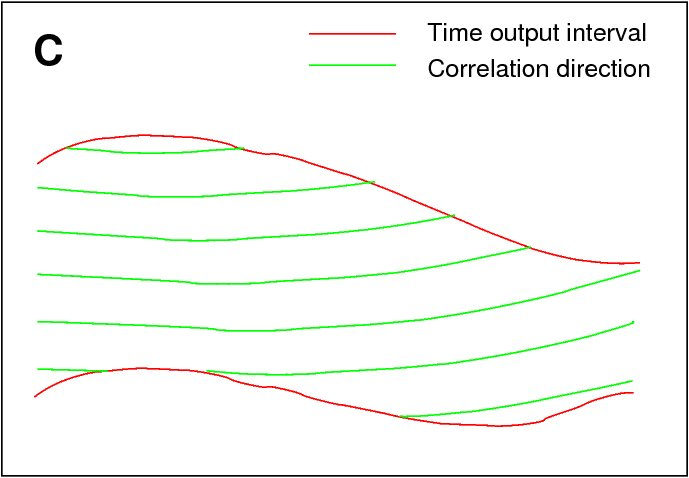
\includegraphics[width=.49\linewidth]{images/C_correlation_parallel_timecut}
  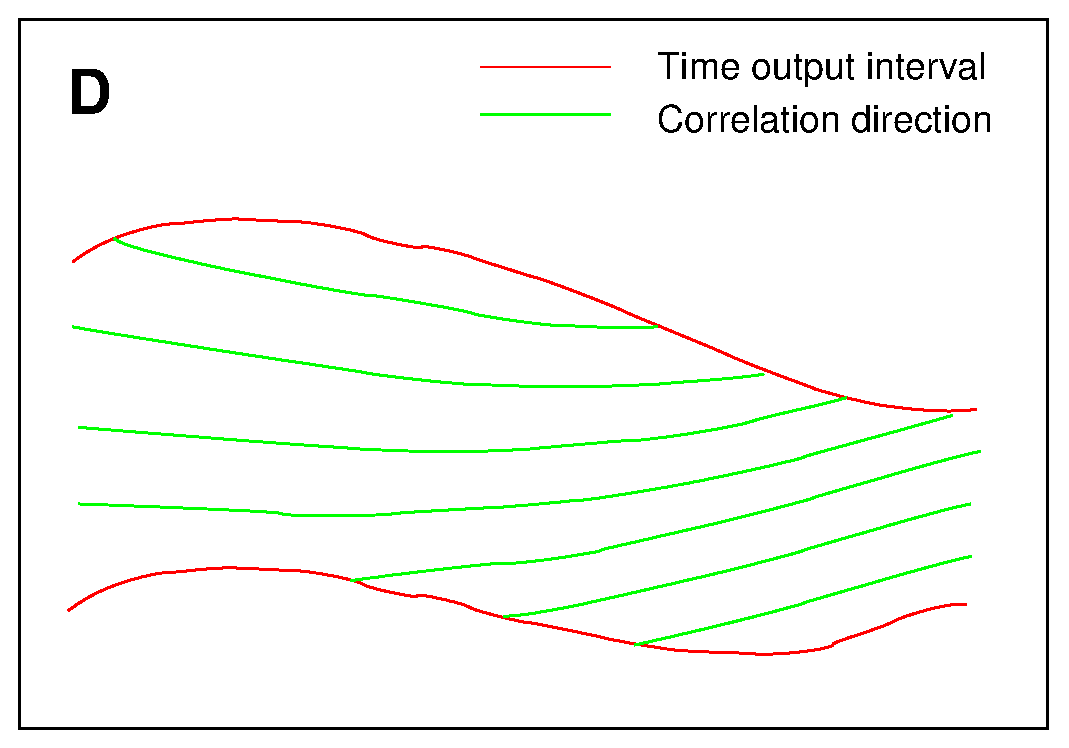
\includegraphics[width=.49\linewidth]{images/D_correlation_proportional_timecut}
  \caption{The layer structure of a (A) parallel top and base,
           (B) top- and base-conform compaction grid (C) Uniform correlation
           structure in a cut grid (D) Compactional correlation structure in a
           cut grid.} 
  \label{fig:inversion-interval-types}
\end{figure}

By specifying a correlation surface, the correlation direction can be
independent of the interval surfaces, see part C of
\autoref{fig:inversion-interval-types} and \autoref{sec:basiccorr}. If
this is done, there are no restrictions on the differences in interval
thickness.

The more flexible approach where a compactional correlation structure
is specified independent of the interval of interest is shown in part D of
\autoref{fig:inversion-interval-types}. 

If only one surface is known, the command \kw{interval-one-surface}
can be used to invert an interval with top and base parallel to this
surface. See \autoref{interval-one-surface} in the reference guide for
more details. Note that depth conversion and correlation surfaces will
not be available in this mode, so the lateral correlation will be
parallel to this surface, as illustrated in part A of
\autoref{fig:inversion-interval-types}. 

\subsubsection{Depth conversion}\label{sec:depthconvusr}
The \kw{output-volume} command is also where the depth conversion is
specified. Additional information for depth conversion has only to be
given under \kw{interval-two-surfaces}, since the lateral area is the
same. To do a depth conversion, one of the 
following must be given: 
\begin{itemize}
\item Reference surface in depth (either top or base), and a velocity cube.
\item Both top and base surface in depth. In this case, we assume constant velocity along each trace, computed from the time and depth surfaces.
\item Both top and base surface in depth, and a velocity cube. In this case, we use the cube for relative velocity in a trace, and scale it to match the interval length.
\end{itemize}

Reference surfaces in depth are given with the tags \kw{depth-file}\kwindex{depth-file} under \kw{top-surface} and/or \kw{base-surface}. The velocity cube can be read from file with the command \kw{velocity-field}\kwindex{velocity-field}. Alternatively, the command \kw{velocity-field-from-inversion}\kwindex{velocity-field-from-inversion} can be used to specify that \vp from inversion should be used for velocity. With depth conversion, the \kw{interval-two-surfaces} command may look like this:
\svex{ex:depthconv}
    <interval-two-surfaces>
      <top-surface>
        <time-file>      FlatTop_3100ms.storm </time-file>
        <depth-file>     FlatTop_3100ms.storm </depth-file>
      </top-surface>
      <base-surface>
        <time-file>      FlatBase_3600ms.storm </time-file>
        <depth-file>     FlatBase_3800ms.storm </depth-file>
      </base-surface>
      <velocity-field>   velocity.storm </velocity-field>
      <number-of-layers>            125 </number-of-layers>
    </interval-two-surfaces>
\end{verbatim}
\end{example}

\subsection{Prior model}
Since seismic data only contain information about relative elastic parameters, the absolute level needs to be set with a background model. In a Bayesian inversion setting, the background model is the prior expectation. We also need the prior covariance, which is given by the covariance of the parameters, the lateral correlation and the temporal correlation, as described in \autoref{sec:statmodthe}. In the model file, all this is gathered under the \kw{prior-model}\kwindex{prior-model} command, which may look something like this:
\svex{ex:priormodel}
<crava>
<prior-model>
  <background>
    <vp-file>      input/background/CravaBgVp.storm  </vp-file>
    <vs-file>      input/background/CravaBgVs.storm  </vs-file>
    <density-file> input/background/CravaBgRho.storm </density-file>
  </background>
  <lateral-correlation>
    <variogram-type> genexp </variogram-type>
    <power>       1 </power>
    <angle>       0 </angle>
    <range>    2500 </range>
    <subrange> 2500 </subrange>
  </lateral-correlation>
</prior-model>
</crava>
\end{verbatim}
\end{example}

\subsubsection{Background model}
\label{sec:basicbg}
The background model is given under the \kw{background}\kwindex{background} command. It can be given from file, using \kw{vp-file}\kwindex{vp-file}, \kw{vs-file}\kwindex{vs-file} and \kw{density-file}\kwindex{density-file}. These files should either be on Storm, crava, Sgri or SegY format. Alternatively, constant values can be used for background model, specified with \kw{vp-constant}\kwindex{vp-constant}, \kw{vs-constant}\kwindex{vs-constant} and \kw{density-constant}\kwindex{density-constant}. Any combinations of files and constants are also accepted. If none of these are given, the background model will be estimated.


Multiinterval (Multizone) background model is achieved by doing a \kw{multiple-intervals} inversion and with estimating background models activated. The surfaces are set under \kw{output-volume}.  It is not possible to  use multiinterval background with a single interval/zone inversion directly. To achieve this, one must first run Crava in estimation mode with \kw{multiple-intervals} and estimate a background model, where the written background model must then be used as input in a single interval inversion. The multiinterval background model will follow the other setting for multiinterval inversion, like \kw{correlation-direction}, \kw{erosion-priority} and \kw{uncertainty}. In each interval, a local background model is created by estimating a depth trend for the zone volume, then interpolating well logs into the depth trends using kriging. The full multiinterval background model is then made by joining the local background models in all the intervals.

\subsubsection{Covariances}
\label{sec:basiccorr}
As shown in \autoref{sec:statmodthe} the prior covariance structure for the elastic parameters consists of three parts:
\begin{enumerate}
\item A 3x3 covariance matrix for point-wise covariance between the parameters. May be read from ASCII file using the command \kw{parameter-correlation}\kwindex{parameter-correlation}.
\item A temporal correlation vector, length equal to number of layers in grid, $n_t$. May be read from ASCII file using the command \kw{temporal-correlation}\kwindex{temporal-correlation}.
\item A lateral correlation structure. May be given as a parametric variogram using the command \kw{lateral-correlation}.
\end{enumerate}
By default, the two first are estimated from well data, and the lateral correlation structure is set to a isotropic exponential variogram with range 1000. The reason for the latter choice is that this is hard to estimate, see \autoref{sec:correstimp} for details. The most common to override is the lateral correlation, where the variogram used for petro-physical modelling is a good choice.
\subsection{Well data}
Unless all information about wavelet, signal to noise and correlations are specified, well data are needed for estimation. Wells are given with the command \kw{well-data}\kwindex{well-data}, and may look like this:
\svex{ex:welldata}
<crava>
<well-data>
  <log-names>
    <time>    TWT  </time>
    <dt>      DT   </dt>
    <dts>     DTS  </dts>
    <density> RHOB </density>
  </log-names>
  <well>
    <file-name> input/logs/ed6406_3-3_cut.rms    </file-name>
  </well>
  <well>
    <file-name> input/logs/ed6506_12-3_cut.rms   </file-name>
  </well>
  <well>
    <file-name> input/logs/ed6506_12-8_cut.rms   </file-name>
  </well>
  <well>
    <file-name> input/logs/ed6506_12-S4H_cut.rms </file-name>
  </well>
</well-data>
</crava>
\end{verbatim}
\end{example}
There are two main elements here. The first is a well log
interpretation, given by \kw{log-names}, which tells \crava which
headers to look for. The following logs are needed: 
\begin{itemize}
\item Two way time log, specified with \kw{time}\kwindex{time}.
\item \vp log, either given by \kw{vp}\kwindex{vp} or \kw{dt}\kwindex{dt}. The latter is used for DT-logs.
\item \vs log, either given by \kw{vs}\kwindex{vs} or \kw{dts}\kwindex{dts}. The latter is used for DTS-logs.
\item Density log, given by \kw{density}\kwindex{density}.
\end{itemize}
In addition, if facies probabilities are computed, a facies log is
needed. This is specified with the tag \kw{facies}\kwindex{facies}. 

The wells are given with the command \kw{file-name} under
\kw{well}\kwindex{well}, which is given once for each well. The reason
for this is that additional information may be given for each
well. Well files should be on NORSAR or RMS-format. 

Each well may be moved to its optimal location using
\kw{optimize-position}\kwindex{optimize-location-to} under
\kw{well}\kwindex{well}, taking the arguments
\rkw{angle}{angle3}\kwindex{angle} and \kw{weight}\kwindex{weight}
which allow the user to assign different weights to the different
angle gathers for each well. The maximum allowed offset and vertical
shift for moving wells is specified in
\kw{maximum-offset}\kwindex{maximum-offset} and
\kw{maximum-shift}\kwindex{maximum-shift} under \kw{well-data}, with
default values of 250 m and 11 ms, respectively. 

The command \kw{synthetic-vs-log} tells whether the \vs log is
synthetic. If not specified, it will be detected from rank correlation
with \vp. The command
\kw{filter-elastic-logs}\kwindex{filter-elastic-logs} is used to do
multi-parameter-filtering of the elastic logs in this well after the
inversion. 

\subsection{I/O settings}
Two commands are used to specify the directory for input files. \kw{top-directory}\kwindex{top-directory} gives the working directory for the model file. 
The command \kw{input-directory}\kwindex{input-directory} is used to specify directory name for root directory for input files. The name is given relative to \kw{top-directory}.

Under \kw{advanced-settings}, the command
\kw{use-intermediate-disk-storage} can be used to limit the memory
usage when running large \crava jobs. A built-in smart-swap is then
activated. The option has largest effect on Microsoft Windows.

Under \kw{project-settings}, \kw{io-settings} and \kw{other-output}, the command \kw{error-file}\kwindex{error-file} writes all errors to a separate file, in addition to the log file. The command \kw{task-file}\kwindex{task-file} writes all tasks to a separate file, in addition to the log file. 
\subsection{Output}
Output is controlled under \kw{io-settings}\kwindex{io-settings} under
\kw{project-settings}. Here, you may set the output directory using
\kw{output-directory}\kwindex{output-directory}, and you may also
specify a prefix for all output files using
\kw{file-output-prefix}\kwindex{file-output-prefix}.

Except for the log file which is placed directly under the
output directory, all files output by crava are placed in
sub-directories. These sub-directories are 

\svex{ex:output-directories}
output-directory / wells 
                 / background 
                 / wavelets 
                 / seismic 
                 / velocity 
                 / correlations 
                 / inversionresults 
\end{verbatim}
\end{example}

There are two main output formats: Grid output, controlled by
\kw{grid-output}\kwindex{grid-output}, and well output controlled by
\kw{well-output}\kwindex{well-output}. The output section may look
something like this: 
\svex{ex:iosettings}
<crava>
<project-settings>
  <io-settings>
    <file-output-prefix> CRAVA_ </file-output-prefix>
      <grid-output>
        <format>
          <segy>       yes </segy>
        </format>
        <domain>
          <time>       yes </time>
          <depth>      yes </depth>
        </domain>
        <elastic-parameters>
          <vp>         yes </vp>
          <vs>         yes </vs>
          <density>    yes </density>
          <background> yes </background>
        </elastic-parameters>
      </grid-output>
      <well-output>
        <wells>         yes </wells>
        <blocked-wells> yes </blocked-wells>
      </well-output>
  </io-settings>
</project-settings>
</crava>
\end{verbatim}
\end{example}

\subsubsection{Grid output}\kwindex{grid-output}
Different elastic parameters can be given as grid output. In addition,
the estimated background model may be written as grids. This is
controlled by the \kw{elastic-parameters}\kwindex{elastic-parameters}
command under \kw{grid-output}. See \autoref{elastic-parameters} for a
full list of possible grids. If this command is not used, \vp, \vs and
density will be written. Output of original and synthetic seismic data
can be given by the \kw{seismic-data}\kwindex{seismic-data}
command. Other grids can be requested for output by the command
\kw{other-parameters}\kwindex{other-parameters}, for example
correlations. 

The grid format may be controlled using \kw{format}\kwindex{format}. Here the yes/no parameters \kw{storm}, \kw{segy}, \kw{sgri}, \kw{crava} and \kw{ascii} can be used to decide if grids should be written on storm- (RMS), segy-, Sgri-, crava- or ASCII-format. You may choose several formats for one run; all grids will be written on all selected formats. The Segy format can be controlled by the \kw{segy-format} command, in the same way as for input data, described in \autoref{sec:basicseis}. Note that correlation grids make sense only in storm format. Default output format is storm. The crava format is a binary format only to be used with \crava. It can be read and written from \crava, and is useful if the output from a \crava run should be used as input to another \crava run because the format is fast to read.

By using the \kw{domain}\kwindex{domain} option, output may be written
in time domain \kw{time} or depth domain \kw{depth} (requires
parameters set under \kw{output-volume}, see
\autoref{sec:depthconvusr}), or both. Again, correlation grids only
make sense in time domain, which is default. 

\subsubsection{Well output}\kwindex{well-output}
Some versions of filtered elastic parameters (\vp, \vs and density) in wells can be generated by the \kw{well-output} command. The wells can be given in two different formats, RMS or NORSAR. This is controlled by the \kw{format}\kwindex{format} command. The logs written are
\begin{itemize}
\item Raw elastic logs.
\item Elastic logs filtered to background frequency.
\item Elastic logs filtered to seismic frequency.
\item Elastic logs filtered with facies prediction filter (if available).
\item Facies log (if available).
\end{itemize}
The wells can either be written with original sampling density, using \kw{wells}, or matching the internal grid resolution, using \kw{blocked-wells}.

\subsection{Actions}
The final information that is needed for a \crava run is what the run is supposed to do. This is controlled by \kw{actions}\kwindex{actions}. The \kw{mode} keyword defines the purpose of this run and should be set to "inversion" when doing inversion. Other options are "estimation", see \autoref{sec:estimateusr} and "forward", see \autoref{sec:forwardusr}. When inversion is chosen, \kw{inversion-settings}\kwindex{inversion-settings} can be used to control basic aspects of the inversion. It may look something like this:
\svex{ex:action}
<crava>
<actions>
  <mode>                    inversion </mode>
  <inversion-settings>
    <prediction>                  yes </prediction>
    <simulation>
      <seed>                   150570 </seed>
      <number-of-simulations>      10 </number-of-simulations>
    </simulation>
  </inversion-settings>
</actions>
</crava>
\end{verbatim}
\end{example}

The command \kw{prediction}\kwindex{prediction} can be used to turn
predictions on or off. By default, the prediction will be generated. A
number of full frequency stochastic realisations of the inversion can
be obtained by specifying \kw{number-of-simulations}\kwindex{number-of-simulations} under \kw{simulation}\kwindex{simulation}. The seed for the random generator can also be given here, with the \kw{seed}\kwindex{seed} command. Changing the seed will give a new set of realisations.

The command \kw{kriging-to-wells}\kwindex{kriging-to-wells} can be
used to krige realisations to well data. By default, this is done if
the \kw{simulation} command is used. 

\subsection{Standard formats for input and output}
\label{sec:gridformats}

\subsubsection{3D-grid}
Crava can read and write the following 3D grid
  formats: SegY, Storm, Sgri (NORSAR) and crava (internal) . On
  output, the format is controlled by a \kw{format} keyword. On input,
  the program automatically detects the format, although it may need
  help to correctly read SegY formats, using the \kw{segy-format}
  keyword. The default output format is storm.

\subsubsection{Surfaces}
The standard format for reading and writing
  surfaces is binary storm, but \crava can also read Roxar ASCII
  surfaces (formerly known as ASCII Irap classic), Multicolumn ASCII
  surfaces (see example below) and XYZ ASCII surfaces. Multicolumn ASCII and XYZ ASCII files must follow the segy geometry.
   In addition some surfaces related to 3D-inversion are read as sgri (NORSAR). On input,
  the surface format will be automatically detected. For writing we currently support Roxar Ascii and Storm binary.
  
\paragraph{Multicolumn Ascii example}
The multicolumn ascii file is a text file with five columns, and each columns needs ta have a header name:
X or UTMX; Y or UTMY; IL or Inline; XL or Crossline; Z, TWT or Attribute. The order of the columns is arbitrary. The file might also have some text before the header-row. This surface is based segy-geometry and must follow the corresponding seismic cube, as the reference point, angle and area are taken from the geometry. We require even sampling in the file, but we do not require as fine sampling as in the seismic. It is for example possible to give only the four corners of the surface. A segy geometry will be required for using multicolumn ascii files. The standard missing value is defined as $-999.25$.

A file may look like:
\begin{table}[h]
\centering
\label{tab:multicolumnascii}
\begin{tabular}{lllll}

X         &         Y              &     Inline       &   Crossline     &    Attribute\\ 
455380.0    &        6799690.0   &        2100.0      &       5600.0       &       2467.05737 \\ 
447256.0    &        6799789.0    &       2100.0       &       5640.0      &        2480.06712\\ 
447393.0    &        6811038.5     &      2120.0      &        5600.0      &        2549.43453\\ 
455517.0    &        6810939.5     &      2120.0      &        5640.0      &        2338.12905\\ 
\end{tabular}
\end{table}

\paragraph{XYZ Ascii example}
The xyz ascii file is a text file with three columns, X, Y and Z. The columns may have a header name, X or UTMX; Y or UTMY; Z, TWT or Attribute. Columns may also be given in an arbitrary order. If there is no header line, it is assumed that the order is x, y, z. This surface is based segy-geometry and must follow the corresponding seismic cube. We require even sampling in the file, but we do not require as fine sampling as in the seismic. It is for example possible to give only the four corners of the surface. A segy geometry will be required for using xyz ascii files. The standard missing value is defined as $-999.25$.

A file may look like:
\begin{table}[h]
\centering
\label{tab:xyzascii}
\begin{tabular}{lll}

X         &         Y              &    Z\\ 
455380.0    &        6799690.0   &        2467.05737 \\ 
447256.0    &        6799789.0    &       2480.06712\\ 
447393.0    &        6811038.5     &      2549.43453\\ 
455517.0    &        6810939.5     &      2338.12905\\ 
\end{tabular}
\end{table}


\subsubsection{Wavelets}
Wavelets are either on JASON or NORSAR format,
  both for reading and writing. Auto-detect is used on reading, use \kw{format3}
  for writing. The default output format is JASON.

\subsubsection{Wells}
For reading we support wells on RMS, NORSAR and LAS format. For writing we currently support RMS and NORSAR. Auto-detect is used on reading; use \kw{format2} to control writing. The default output format is RMS.

\section{Advanced inversion options}
\label{sec:advinvusr}
Although \crava is mainly intended as a simple and fast inversion
tool, there are still some options to control the inversion, and to
access more sophisticated approaches. Most of these are covered here,
see 
also \autoref{advanced-settings} for details about
\kw{advanced-settings}. 
\subsection{Non-stationary wavelet and noise}
Although the FFT-algorithm which is at the core of \crava requires
stationarity, this does not mean that the entire inversion has to be
stationary, as discussed in \autoref{sec:nonstationaryimp}. We allow
lateral variations in wavelet amplitude, wavelet shift and signal to
noise ratio.

The local wavelet transformations fit well within the core framework
of \crava, but the local noise requires some approximations, as
explained in section \autoref{sec:localnoiseimp}. This means that
local noise only improves the final result if the local variations are
substantial. We do not recommend using local noise if the variation in
noise level is less than 15\%.

Unlike the basic level, where parameters that were not specified 
automatically got estimated, the use of local wavelets or local noise
must be explicitly triggered. For wavelets, this is done with the
\kw{local-wavelet}\kwindex{local-wavelet} command under
\kw{wavelet}. There are four alternatives:
\kw{local-wavelet}: 
\begin{enumerate}
\item \kw{shift-file} gives a file name for a map giving the local shifts. 
\item \kw{estimate-shift} will estimate a local shift map when set to "yes".
\item \kw{scale-file} gives a file name for a map giving the local scale. 
\item \kw{estimate-scale} will estimate a local scale map when set to "yes".
\end{enumerate}
Naturally, the shift can not be both given and estimated, the same
holds for scale. Note that you may choose to use only shifts, omitting
both scale keywords, or use only scale. 

The local noise is triggered similarly, by using one of two
commands under \kw{angle-gather}: 
\begin{enumerate}
\item \kw{local-noise-scaled} gives a file name for a map with the local scaling of
  the signal to noise ratio.
\item \kw{estimate-local-noise} estimates the local scaling of the
  signal to noise ratio if set to "yes". 
\end{enumerate}

\subsection{PS-seismic and reflection approximations}
By default, \crava assumes that the input seismic data are PP, but PS
data can also be used. For both cases, we use the linearised
Aki-Richards approximation, see \autoref{eq:aki_c}. The type of seismic data is
indicated by using the \kw{type}\kwindex{type} command
under\kw{seismic-data}. Here, \kw{type} should be either "pp" or
"ps". Note that PS data must also be aligned in PP-travel time, as no
such alignment is done internally by \crava. 

Instead of using the default reflection approximation, the user may
supply the parameters to compute the reflections. We always assume
that for a given angle and seismic type, the reflections can be
computed from the equation 
\begin{equation}
\begin{split}
  c(\vect{x},t,\theta)
  & = a_{V\!p} (\theta) \frac{\partial}{\partial t}\ln\vp (\vect{x},t)\\
  & + a_{V\!s} (\vect{x},t,\theta) \frac{\partial}{\partial t}\ln\vs (\vect{x},t)\\
  & + a_\rho(\vect{x},t,\theta) \frac{\partial}{\partial t}\ln\rho(\vect{x},t).
\label{eq:linrefl}
\end{split}
\end{equation}
The coefficients $a_{V\!p}$, $a_{V\!s}$ and $a_\rho$ can be read from
file, using the \kw{reflection-matrix}\kwindex{reflection-matrix}
command under \kw{advanced-settings}. This file should have one line
for each seismic data file, and each line should have the three
coefficients for one set of seismic input data. The order of the lines
should be the same as the order of the seismic data in the \kw{survey}
command. 

\subsection{Well quality checks}
Well logs are often faulty, and \crava has some safety mechanisms to
detect this. The primary mechanism is to detect extreme values, and
set these undefined. The default upper and lower bounds accepted in
well logs are shown in \autoref{tab:logminmax}. These can be
overridden using the command 
\kw{allowed-parameter-values}\kwindex{allowed-parameter-values} under
\kw{well-data}. Here, \kw{minimum-vp}, \kw{minimum-vs},
\kw{minimum-density} and the corresponding maximum values can be
given. 
\begin{table}
\caption{Default intervals for valid well log values.\label{tab:logminmax}}
\begin{tabular}{|lrr|}
\hline
& Min & Max \\
\hline
\vp & 1300 & 7000 \\
\vs &  200 & 4200 \\
$\rho$ & 1.4 & 3.3 \\
\hline
\end{tabular}
\end{table}

Some logs may stay within reasonable values, but have too much or too
little variation, also indicating that something is wrong. We
therefore calculate the variance of the logarithm of the log minus the
background, and if this is outside reasonable bounds, an error is
triggered. The default bounds shown in \autoref{tab:logvarminmax} can
be overridden with \kw{allowed-parameter-values}, using
\kw{minimum-variance-vp}, and so forth. 
\begin{table}
\caption{Default intervals for valid well log variances.\label{tab:logvarminmax}}
\begin{tabular}{|lrr|}
\hline
& Min & Max \\
\hline
Var(ln(\vp)) & $5*10^{-4}$ & $250*10^{-4}$ \\
Var(ln(\vs)) & $10*10^{-4}$ & $500*10^{-4}$ \\
Var(ln($\rho$)) & $2*10^{-4}$ & $100*10^{-4}$ \\
\hline
\end{tabular}
\end{table}

\subsection{Generate synthetic seismic from inversion data}
It is possible to generate synthetic seismic by a forward modelling
with the \vp, \vs and density resulting from the inversion. This is done
by the command  \kw{synthetic} under \kw{seismic-data} under
\kw{grid-output}, \kw{io-settings},  in command
\kw{project-settings}. 

\section{Estimation}
\label{sec:estimateusr}
As mentioned, \crava can estimate many of the needed parameters. There
are several commands that control the estimation behaviour for
wavelets, noise and background model. Note that the correlations will
always be estimated as explained in \autoref{sec:correstimp} from all
available well logs, and do not have any further controls. 

\subsection{Estimation mode}
If you only want to do the estimation, in order to check the quality
of the estimates, you can use "estimate" in the \kw{mode}
command. Using this, \crava will perform the initial model building
tasks and estimate needed information, but terminate once all
information needed for inversion is estimated. When running in
estimation mode, you can also control the main estimation aspects
using the \kw{estimation-settings}\kwindex{estimation-settings}
command. This allows you to control which of the main estimation tasks
should be carried out, setting yes or no for
\kw{estimate-correlations}, \kw{estimate-wavelet-or-noise} or
\kw{estimate-background}. Parameters with a "no" will not be estimated
unless needed for other estimations. Note that in estimation mode, all
estimated parameters are written to file, regardless of output
settings. 
\subsection{Wavelet and noise estimation}
Wavelets and noise are estimated together. These parameters will only
be estimated from wells that are vertical or close to vertical, since
this allows comparing synthetic seismic from well logs with one or a
couple of traces, and thus reduces alignment issues. The angle limit
can be controlled by the
\kw{maximum-deviation-angle}\kwindex{maximum-deviation-angle} command
under \kw{well-data}. In addition, wells can be excluded individually,
by setting \kw{use-for-wavelet-estimation} to "no" under \kw{well}. 

By default, the wavelet and noise are estimated in the region between
the top and base surface for the inversion area. This may be limited
using the \kw{wavelet-estimation-interval} command under 
\kw{survey}, where a separate set of restricting surfaces are given
with \rkw{top-surface}{top-surface3}, \rkw{time-file}{time-file3} and 
\rkw{base-surface}{base-surface3}, \rkw{time-file}{time-file3}. It is
also possible to specify these restrictions a contant value, using
the \rkw{time-value}{time-value3} keyword. Since these are
under \kw{wavelet}, they can be different for each angle. 

Some wavelet estimation options are also found under the command
\kw{advanced-settings} given under \kw{project-settings}. These are 
\begin{itemize}
\item \kw{wavelet-tapering-length} which controls the length of the wavelet (in ms).
\item \kw{minimum-relative-wavelet-amplitude} which finds the wavelet
  length, by setting the cutoff size for edge peaks relative to centre
  peak. 
\item \kw{maximum-wavelet-shift} which controls how far the wavelet
  can be shifted locally, see \autoref{sec:waveestimp}. 
\end{itemize}

Prior information for local wavelet modelling is given by the
\kw{local-wavelet} command under \kw{prior-model}. Here, lateral
correlation is specified as  a 2D variogram for the lateral
correlation in local wavelet modelling by the command
\kw{lateral-correlation}. 

Output of wavelets is controlled by the \kw{wavelet-output}\kwindex{wavelet-output} command under \kw{io-settings}. 
Two different formats can be specified, JASON and NORSAR. Estimated wavelets for each well is written by the 
\kw{well-wavelets}\kwindex{well-wavelets} command. The command \kw{global-wavelets}\kwindex{global-wavelets} 
writes global wavelets for each seismic angle. If local wavelet is requested, the command 
\kw{local-wavelets}\kwindex{local-wavelets} writes estimated local wavelet shift and scale surfaces.

Output of estimated local noise surface is given by the command
\kw{local-noise} given under \kw{io-settings} and \kw{other-output}. 

\subsection{Background model estimation}
The background model is estimated as a low frequency vertical
trend. The trend is given in relative depth in the inversion volume,
so the trend value along the top and base surface is constant. At
well locations, the trend is kriged to the well logs. By default, all
wells are used for background model estimation, but can be excluded by 
specifying "no" for \kw{use-for-background-trend} under \kw{well} for individual
wells. 

The background estimation can be controlled by some commands under
\kw{background}\kwindex{background}. These are: 
\begin{itemize}
\item \kw{velocity-field} takes an external velocity field, typically
  from migration, and uses as \vp background, kriged to low frequency
  \vp well logs. 
\item \kw{lateral-correlation} gives a variogram for the
  kriging. Larger ranges extends the influence of well data further
  away from wells. 
\item \kw{high-cut} allows specification of a maximum frequency for
  the background model. 
\end{itemize}

\subsection{Prior correlations}
Prior correlations between \vp, \vs and density, and autocorrelation are estimated. they can be written to file by the command \kw{prior-correlations}\kwindex{prior-correlations} under \kw{project-settings}, \kw{io-settings} and \kw{other-output}.

\section{3D wavelet}
Instead of the traditional 1D wavelet a 3D wavelet can be used in
\crava. This wavelet is constructed by a 1D pulse and a 3D wavelet
filter based on illumination vectors. The use of a 3D wavelet is
invoked by the keyword \kw{wavelet-3d}.  

The 1D pulse used to construct the 3D wavelet, can be specified by the
\kw{file-name} keyword. If a file is not specified, this pulse is
estimated. Either way, a filter file must be given by the keyword
\kw{processing-factor-file-name}. This filter contains the amplitude
effects related to the illumination vectors and is given on Sgri
format. One or two filters are given. The first, and necessary,
contains frequency-independent amplitude effects, while the second, if
given, contains frequency-dependent amplitude effects. 

For noise estimation in the 3D wavelet setting, a propagation filter
file is given by the keyword \kw{propagation-factor-file-name}. At
present, this is not used. The keyword \kw{stretch-factor} can be
given, but is not used since the stretch factor is automatically
calculated from the offset angle. 

When estimating the 1D pulse, seismic data from a neighbourhood of the
well can be used. The distance from the well, specified in meters,
that data are collected is given by the commands
\kw{estimation-range-x-direction} and
\kw{estimation-range-y-direction}. The default is that only data from
the well position are used.   

When 3D wavelet is used, certain parameters related to the mapping
between time and depth are needed. This occurs since the illumination
vectors relates to depth, while \crava works in time. These
settings are given under keyword
\kw{time-to-depth-mapping-for-3d-wavelet} in \kw{project-settings}. A 
reference depth for the target area must be specified under the keyword
\kw{reference-depth}. This depth represents a constant surface which 
in time normally will refer to a variable surface due to varying
velocity above this depth. This reference surface is given by
\kw{reference-time-surface} and can be given on Storm- or
Sgri-format. The parameter \kw{average-velocity} refers to the average
velocity in the target area which is needed for the estimation of the
pulse.  

\section{Rock physics}
\label{sec:rockPhysics}
The idea behind the rock physics template is to be able to model the density and elastic properties of a fluid-filled \kw{rock} in a very flexible way, by selecting from and possibly combining many different rock physics theories. In order to do this, we need some basic building blocks. The basic building blocks here are \kw{fluid}, \kw{solid}, \kw{dry-rock} (a solid with porosity, but no fluid) and \kw{rock} (a combination of solid and fluid).

In \crava, the rock physics models are used for generating the background model and covariance matrix used in the prior model, and for generating synthetic wells used for facies estimation. 

\subsection{Structure of the rock physics template}
The base structure of the rock physics template consists of the elements \kw{reservoir}, \kw{evolve}, \kw{predefinition}, \kw{rock} and \kw{trend-cube}, each of which contains sub-elements.

The sub-elements will be basic building blocks (e.g. \kw{solid}, \kw{fluid}, \kw{dry-rock}), properties (e.g. temperature, pore-pressure, density, etc) and theories.

\subsubsection{Reservoir}
\kw{reservoir} contains reservoir properties, such as pressure, temperature, porosity, fluid saturation, lithology, etc. Reservoir properties given under the keyword \kw{reservoir} are parameters common for fluids, solids, dry rocks and rocks. For models that depend on these parameters, the values given under reservoir can be used, although they may be overridden locally. The elements in \kw{reservoir} are defined by labels to be referred to with the \kw{reservoir-variable} statement. Hence, they must be unique. 
After \kw{reservoir}, the command \kw{variable} follows. Below is an example of how \kw{reservoir} can be defined:
\svex{ex:Reservoir}
<reservoir>
  <variable>
    <label> temperature </label>
    <value> 50 </value>
  </variable>

  <variable>
    <label> porosity </label>
    <gaussian>
      <mean> 0.5 </mean>
      <variance> 0.1 </variance>
    </gaussian>
  </variable>
</reservoir>
\end{verbatim}
\end{example}

\subsubsection{Evolve}
\kw{evolve} controls the time development of the reservoir variables. Under the keyword \kw{evolve}, \rkw{reservoir-variable}{reservoir-variable-evolve}, \kw{one-year-correlation} and \rkw{vintage}{vintage-evolve} are given. \kw{reservoir-variable} needs to be the label of one of the variables defined in \kw{reservoir}. \kw{one-year-correlation} defines the correlation between the reservoir variable at two following years. \rkw{vintage}{vintage-evolve} is repeated for each vintage of the time development. In \rkw{vintage}{vintage-evolve}, \rkw{distribution}{distribution-vintage} and \kw{vintage-year} are given. \rkw{distribution}{distribution-vintage} is the distribution of the reservoir variable at the given vintage, and it needs to be one of the distributions given under \kw{value-assignments}. \kw{vintage-year} is the year of the given vintage of the reservoir variable.
Below is an example with \kw{evolve} for the reservoir variable porosity:
\svex{ex:evolve}
<evolve>
  <reservoir-variable> porosity </reservoir-variable>
  <one-year-correlation> 0.7 </one-year-correlation>
  <vintage>
    <distribution>
      <beta>
        <mean> 0.1 </mean>
        <variance> 0.01 </variance>
      </beta>
    </distribution>
    <vintage-year> 2000 </vintage-year>
  </vintage>

  <vintage>
    <distribution>
      <beta>
        <mean> 0.08 </mean>
        <variance> 0.01 </variance>
      </beta>
    </distribution>
    <vintage-year> 2002 </vintage-year>
  </vintage>
</evolve>
\end{verbatim}
\end{example}

\subsubsection{Predefinitions}
\kw{predefinitions} is used for specifying and calculating the elastic properties of basic building blocks, being \kw{solid}, \kw{fluid} or \kw{dry-rock}, or elements and mixtures of these. It will typically use properties specified under \kw{reservoir}. 

Each time a building block is defined, it is given a unique identifying name using the \kw{label} keyword. This is followed by a keyword specifying which theory we use for building this element, and inside that keyword block, the required parameters for the theory are given. 

Inside the theory block, the required parameters for the theory are given. 
The theories are used for calculating the bulk and shear moduli. In addition, they are implicitly used for calculating the density using the arithmetic average of the constituent densities. 

If we want to use an element that is already defined, we can use the keyword \kw{use} instead of \kw{label}, followed by the unique name of the element. Thus, we can easily reuse elements once they are defined.

The significant difference between elements in \kw{reservoir} and \kw{predefinitions} is that each element in \kw{reservoir} defines a single property, while it defines an object with several properties in \kw{predefinitions} (e.g. bulk modulus, shear modulus and density). These objects are typically used as inputs to various theories for calculating the effective properties of a mixed material.

\svex{ex:predefinitions}
<predefinitions>
  <solid>
    <label> quartz </label>
    <tabulated>
      <bulk-modulus> 37 </bulk-modulus>
      <shear-modulus> 44 </shear-modulus>
      <density> 2.65 </density>
    </tabulated>
  </solid>
  <fluid>
    <label> brine </label>
    <batzle-wang-brine>
      <pore-pressure> 20 </pore-pressure>
      <temperature> 60 </temperature>
      <salinity> 0.05 </salinity>
    </batzle-wang-brine>
  </fluid>
</predefinitions>
\end{verbatim}
\end{example}

\subsubsection{Rock}
\kw{rock} contains the final composition of the rock, and will typically use details specified in \kw{reservoir} and \kw{predefinitions}. The \kw{rock} command is followed by either \kw{label} or \kw{use}. If \kw{label} is used, the next keyword is a theory. 

The rocks to be used in the facies estimation, need to correspond to the facies given in \kw{facies-probabilities}.

Example:

\svex{ex:rock}
<rock>
  <label> effective rock </label>
  <gassmann>
    <dry-rock>
      <use> quality sand </use>
    </dry-rock>
    <fluid>
      <use> brine </use>
    </fluid>
  </gassmann>
</rock>
\end{verbatim}
\end{example}

\subsubsection{Trend cubes}
<trend-cube> contains the trend cubes that can be used for defining a trend on the variables. Each variable defined by a trend may be related to one or two trend cubes. These trend cubes may for example be related to time and depth, and they need to be defined in the entire inversion volume. 

\subsection{Value assignments in the rock physics template}
All the properties and function parameters can use previously assigned values defined in <reservoir>, or be assigned values directly in <predefinitions>. The possible types of value assignments are value, trend or distribution. 

\subsubsection{Value}
The simplest form of deterministic value assignment is a single value. For the variables in <reservoir>, the value is given by the command <value>, while it may be given directly for the variable commands of <predefinitions>. Below is an example for each of these cases:
\svex{ex:assignValue}
<reservoir>
  <variable> 
    <label> temperature </label>
    <value> 40 </value>
  </variable>
</reservoir>

<predefinitions>
  <solid>
    <label> clay </label>
    <tabulated>
      <bulk-modulus> 21 </bulk-modulus>
      <shear-modulus> 7 </shear-modulus>
      <density> 2.6 </density>
    </tabulated>
  </solid>
</predefinitions>
\end{verbatim}
\end{example}

\subsubsection{Distributions}
The rock physics template supports the distribution functions \kw{gaussian}, \kw{beta} and \kw{beta-end-mass} for assigning probabilistic values to a variable. Whenever several building blocks use the same stochastic variable defined under <reservoir>, the same sample of the variable is used for all the building blocks. The required input variables for the different distributions are given in \autoref{sec:valueassignment}.

Examples:
\svex{ex:assignDistribution}
<reservoir>
  <variable>
    <label> total-porosity </label>
    <gaussian>
      <mean> 0.25 </mean>
      <variance> 0.05 </variance>
    </gaussian>
  </variable>

  <variable>
    <label> bulk-quartz </label>
    <beta>
      <mean> 63000000 </mean>
      <variance> 30000 </variance>
      <lower-limit> 10000000 </lower-limit>
      <upper-limit>100000000</upper-limit>
    </beta>
  </variable>
</reservoir>
\end{verbatim}
\end{example}

\subsubsection{Assigning trends to the rock physics variables}
\label{sec:assigntrendsrockphy}
The values of the variables may be given by a trend. The trends are named \kw{trend-1d} or \kw{trend-2d}, with the 1d and 2d endings telling if the property values should be related to one or two trend cubes. These trend cubes may for example be related to time and depth, and they need to be defined in the entire inversion volume. If the trend is to be used, trend cubes must be given on the same level as \kw{reservoir} using the command \kw{trend-cube} following the example below. 
If the trend represent a mean or a variance (as in for example the background model), these can be estimated from data by specifying either \kw{mean} or \kw{variance} in  addition to using the command \kw{estimate}. Note that if the model is 1-dimensional, it is necessary to specify the reference parameter, see the examples below. The estimation methods are version of standard kernel smoothing (local linear regression for the mean and a weighted kernel smoothing for the variance). Note that the mean and variance does not need to have the same dimensionality, see the examples below.


\svex{ex:assignTrend}
<reservoir>
  <variable> 
    <label> temperature </label>
    <trend-1d>
      <file-name> trend1d.txt </file-name>
      <reference-parameter> time </reference-parameter>
    </trend-1d>
  </variable>

  <variable> 
    <label> porosity </label>
    <trend-2d> 
      <file-name> trend2d.txt </file-name>
      <reference-parameter-first-axis> time 
      </reference-parameter-first-axis>
      <reference-parameter-second-axis> depth 
      </reference-parameter-second-axis>
    </trend-2d>
  </variable>
</reservoir>

<trend-cube>
  <parameter-name> time </parameter-name>
  <file-name> trendCubeTime.txt </file-name>
</trend-cube>

<trend-cube>
  <parameter-name> depth </parameter-name>
  <file-name> trendCubeDepth.txt </file-name>
</trend-cube>

<vp>
  <gaussian>
    <mean>
      <trend-2d>
        <estimate>yes</estimate>
      </trend-2d>
    </mean>
    <variance>
      <trend-1d>
       <estimate>yes</estimate>
        <reference-parameter>twt</reference-parameter>
      </trend-1d>
    </variance>
  </gaussian>
</vp>

<vp>
  <gaussian>
    <mean>
      <trend-1d>
        <estimate>yes</estimate>
        <reference-parameter>twt</reference-parameter>
      </trend-1d>    
    </mean>
    <variance>
      <estimate>yes</estimate>      
    </variance>
  </gaussian>
</vp>

\end{verbatim}
\end{example}


\section{Facies prediction}
An important feature in \crava is the ability to create facies
probabilities. This requires that \kw{mode} is set to "inversion", and
is triggered by the \kw{facies-probabilities} command under
\kw{inversion-settings}. 
%The value given here should be either
%"absolute" or "relative", corresponding to probability computations
%based on absolute or relative inverted parameters. 


The facies probabilities are computed based on the inversion results
and a distribution for inversion values given facies computed from
filtered well logs, where the filter is defined by the inversion. See
\autoref{sec:facprobthe}. Probability volumes will be computed for all
facies seen in wells, and if the command
\kw{facies-probabilities-with-undef}\kwindex{facies-probabilities-with-undef}
is used, an additional undefined probability cube is
also generated, indicating areas where the inversion values are too
far away from well data to make reliable predictions. 

Except from the trigger in \kw{inversion-settings}, all parameters
related to facies probabilities are given under
\kw{facies-probabilities}\kwindex{facies-probabilities} under
\kw{prior-model}. Here is an example: 
\svex{ex:facprob}
<crava>
<prior-model>
  <facies-probabilities>
    <use-vs>                          yes </use-vs>
    <use-prediction>                  yes </use-prediction>
    <use-absolute-elastic-parameters> yes </use-absolute-elastic-parameters>
    <estimation-interval>
      <top-surface-file>  input/horizons/facies_top.storm  </top-surface-file>
      <base-surface-file> input/horizons/facies_base.storm </base-surface-file>
    </estimation-interval>
    <prior-probabilities>
      <facies>
        <name>          sand </name>
        <probability>    0.4 </probability>
      </facies>
      <facies>
        <name>         shale </name>
        <probability>    0.6 </probability>
      </facies>
    </prior-probabilities>
  </facies-probabilities>
</prior-model>
</crava>
\end{verbatim}
\end{example}

\begin{figure}[h]
  \centering
  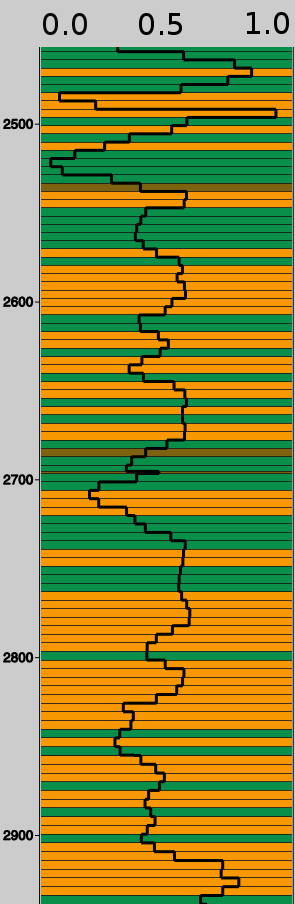
\includegraphics[width=.305\linewidth, height=100mm]{images/sand_probability_well_off}\qquad
  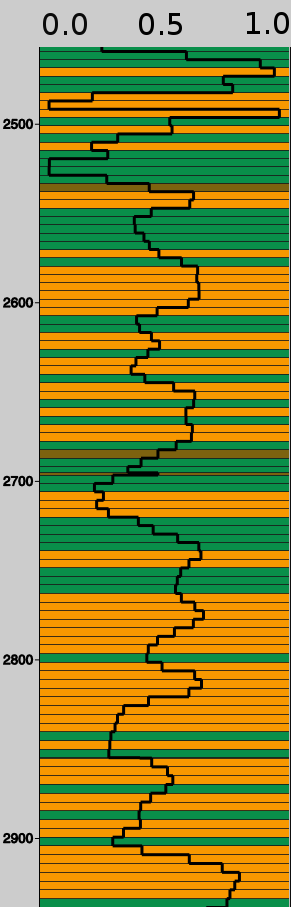
\includegraphics[width=.300\linewidth, height=100mm]{images/sand_probability_well_on}
  \caption{A sample facies probability estimation. The black curve gives the
    probability of sand in a well containing sand (orange), shale
    (green) and crevasse (brown). In the left figure the well was not
    included in the facies probability estimate whereas it was
    included in the right figure.} 
  \label{fig:sandprob}
\end{figure} 

If \kw{use-absolute-elastic-parameters} is set to 'yes', facies probability is computed based on
inverted parameters including background model.
If the distribution
for elastic parameters for each facies is constant over the inversion
volume, using absolute values is more stable. However, if there are
trends in the elastic parameters, the relative values are more
robust. The default is to use relative values.

%Instead of \kw{probability}, we can use \kw{probability-cube}, where
%prior facies probabilities are given on a file. A prior value for
%undefined facies is set with the command \kw{uncertainty-level}. 

The interval to use for facies probability calculations can be
set with \kw{estimation-interval}, similar to
estimation interval for wavelets. Parallel to the wavelet case, wells
may also be excluded using the \kw{use-for-facies-probabilities}
command under \kw{well}.

\subsection{Prior probabilities}
In order to get reliable probabilities, we need good prior
probabilities. By default, \crava computes the average fraction of
each facies in the relevant interval of the wells. This can be
overridden using the \kw{prior-probabilities} command, which
allows specification of these. Note that probabilities must be given
for each facies. Probabilities can either be given globally, with
\kw{probability}, or as a full 3D trend, using
\kw{probability-cube}. The latter takes a grid file as argument,
and the corresponding grid must cover the inversion volume.
A prior value for
undefined facies is set with the command \kw{uncertainty-level}. 

\subsection{Output parameters}
Facies probabilities can be written to file by using the command
\kw{facies-probabilities}\kwindex{facies-probabilities} or
\kw{facies-probabilities-with-undef}\kwindex{facies-probabilities-with-undef}
given under \kw{project-settings}, \kw{io-settings},  
\kw{grid-output} and \kw{other-parameters}. \kw{facies-probabilities} gives probabilities for
the existing facies that sum up to one. This is recommended for use in
RMS. \kw{facies-probabilities-with-undef} includes probability for
undefined facies, and this cube will be the most correct
one. \kw{facies-likelihood}\kwindex{facies-likelihood} writes the
likelihood for inverted seismic for each facies, $p(m|f)$, while
\kw{seismic-quality-grid}\kwindex{seismic-quality-grid} writes a grid
kriged from values for fit between facies probabilities and facies
observed in each of the wells. 

Rock physics distributions can be written by the command
\kw{rock-physics-distributions}\kwindex{rock-physics-distributions}
under \kw{io-settings} and \kw{other-output}. The distributions are
written per facies, with \vp, \vs and density as
axes. The density axis is scaled by a factor of 1000, to make zooming easier in RMS, and in order to have sufficient resolution in SEGY. The density is scaled by a factor 1 000 000, again for SEGY convenience.


\section{Forward modelling}
\label{sec:forwardusr}
A minor functionality in \crava is that it can do forward modelling,
showing what seismic response the program would expect from a given
set of elastic parameters. This is triggered by using "forward" as
\kw{mode}. In this mode, we generate synthetic seismic data from the
given background volumes. A file for forward modelling looks like this: 
\svex{ex:forward}
<crava>
<actions>
  <mode> forward </mode>
</actions>

<survey>
  <angle-gather>
    <offset-angle>  0 </offset-angle>
    <wavelet>
      <file-name> wavelets/ricker.txt      </file-name>
    </wavelet>
  </angle-gather>

  <angle-gather>
    <offset-angle> 10 </offset-angle>
    <wavelet>
      <file-name> wavelets/rickershift.txt </file-name>
    </wavelet>
  </angle-gather>
</survey>

<prior-model>
  <earth-model>
    <vp-file>      background/Vp.storm  </vp-file>
    <vs-file>      background/Vs.storm  </vs-file>
    <density-file> background/Rho.storm </density-file>
  </earth-model>
</prior-model>

<project-settings>
  <output-volume>
    <!-- Lateral dimensions are extracted from the volume for Vp -->
    <interval-two-surfaces>
      <top-surface>
        <time-file> horizons/top.irap  </time-file>
      </top-surface>
      <base-surface>
        <time-file> horizons/base.irap </time-file>
      </base-surface>
      <number-of-layers>           250 </number-of-layers>
    </interval-two-surfaces>
  </output-volume>

  <io-settings>
      <grid-output>
        <format>
          <segy> yes </segy>
        </format>
      </grid-output>
  </io-settings>

</project-settings>
</crava>
\end{verbatim}
\end{example}
Note that no seismic files are given under \kw{survey}, as these are
now computed. No wells are used, since nothing can be estimated
here. We need the angles to generate seismic data for, the
corresponding wavelets, the elastic parameters (given as earth model),
and the volume. Instead of using one of the commands defining volume,
the volume can be taken from \vp.  The output format can be controlled
using \kw{io-settings}, as can input- and output-directory. Other
input will be ignored. 


\newpage

\chapter{CRAVA model file reference manual}\index{reference manual, CRAVA model file elements}
\label{ap:model-file-reference}
\index{CRAVA model file@Crava model file!reference manual for elements}
The numbering shows the command grouping. A command with no sub-numbering expects a value to be given, otherwise, it is only a grouping of other commands.

File names are currently given with a path relative to the directory settings in <project-settings>-<io-settings>-<input/output/top-directory>. If these are not given, the path will always be relative to the working directory.

All commands are optional, unless otherwise stated. A necessary command under an optional is only necessary if the optional is given.

Standard grid formats for surfaces and 3D grids are given in \autoref{sec:gridformats}.

\section{\hbracket{actions}\necessary} \newkw{actions}
 \slist
   \item \Description Controls the main purpose of the run.
   \item \Argument Elements specifying the main purpose
 \elist

\subsection{\hbracket{mode}\necessary}  \newkw{mode}
 \slist
   \item \Description Inversion:\index{inversion!mode} Invert seismic input data to elastic parameters and/or facies probabilities. Needs seismic data and volume, all other missing data will be estimated.
Forward:\index{forward!mode} Create seismic response from background model. Not able to estimate anything.
Estimation:\index{estimation!mode} Checks input data and performs estimation of lacking information for inversion, but stops before inversion.
   \item \Argument 'inversion', 'forward' or 'estimation'
 \elist

\subsection{\hbracket{inversion-settings}}  \newkw{inversion-settings}
 \slist
   \item \Description Controls aspects of the inversion. Only valid with the \kw{mode} 'inversion' above.
   \item \Argument Elements controlling the inversion
   \item \Default
 \elist

\subsubsection{\hbracket{prediction}}  \newkw{prediction}
 \slist
   \item \Description Controls whether predicted elastic parameters will be generated.
   \item \Argument 'yes' or 'no'
   \item \Default
 \elist

\subsubsection{\hbracket{simulation}}  \newkw{simulation}
 \slist
   \item \Description Controls aspects of the simulation of elastic parameters.
   \item \Argument Elements controlling the simulation of elastic parameters
 \elist



\paragraph{\hbracket{seed}}  \newkw{seed}
 \slist
   \item \Description A number used to initialise the random generator. Running a model file with a given seed will give the same simulation results each time.
   \item \Argument Integer
   \item \Default 0
 \elist

\paragraph{\hbracket{seed-file}}  \newkw{seed-file}
 \slist
   \item \Description Alternative to \kw{seed}. This is an ASCII file containing a number. At the termination of the run, the file will be overwritten with a seed generated by the random generator. Thus, a model file using this will generate different simulation results on sequential runs.
   \item \Argument ASCII file containing a number
   \item \Default
 \elist

\paragraph{\hbracket{number-of-simulations}}  \newkw{number-of-simulations}
 \slist
   \item \Description Integer value giving the number of stochastic realizations to generate.
   \item \Argument Integer
   \item \Default 0
 \elist

\subsubsection{\hbracket{kriging-to-wells}}  \newkw{kriging-to-wells}
 \slist
   \item \Description Should the realizations be kriged to well data?
   \item \Argument 'yes' or 'no'
   \item \Default 'yes' if not the \kw{simulation} command is used.
 \elist

\subsubsection{\hbracket{facies-probabilities}}  \newkw{facies-probabilities}
 \slist
   \item \Description Should facies probabilities be estimated?
   \item \Argument 'yes' or 'no'
   \item \Default 'no'
 \elist




\subsection{\hbracket{estimation-settings}} \newkw{estimation-settings}
 \slist
   \item \Description Controls what will be estimated. Only valid with the \kw{mode} 'estimation'. Note that these commands can only turn off estimations - a parameter that is given will not be estimated even if it says so here.
   \item \Argument Elements controlling what to estimate
   \item \Default
 \elist

\subsubsection{\hbracket{estimate-background}}  \newkw{estimate-background}
 \slist
   \item \Description If 'no', background will not be estimated unless needed for other estimation.
   \item \Argument 'yes' or 'no'
   \item \Default 'yes'
 \elist

\subsubsection{\hbracket{estimate-correlations}}  \newkw{estimate-correlations}
 \slist
   \item \Description If 'no', correlations will not be estimated unless needed for other estimation.
   \item \Argument 'yes' or 'no'
   \item \Default 'yes'
 \elist

\subsubsection{\hbracket{estimate-wavelet-or-noise}}  \newkw{estimate-wavelet-or-noise}
 \slist
   \item \Description If 'no', wavelets and/or noise will not be estimated unless needed for other estimation.
   \item \Argument 'yes' or 'no'
   \item \Default 'yes'
 \elist

 \section{\hbracket{project-settings}\necessary} \newkw{project-settings}
 \slist
   \item \Description Controls inversion volume, output and advanced program settings.
   \item \Argument Elements controlling inversion volume, output and advanced program settings
   \item \Default
 \elist

\subsection{\hbracket{output-volume}\necessary} \newkw{output-volume}
 \slist
   \item \Description Defines the core inversion volume. All grid output will be given in this volume.
   \item \Argument Elements defining the core inversion volume.
   \item \Default
 \elist

\subsubsection{\hbracket{interval-two-surfaces}} \newkw{interval-two-surfaces}
 \slist
   \item \Description One way to give the top and bottom limitations. Must be used if output in depth domain is desired. This or \kw{interval-one-surface} must be given.
   \item \Argument
   \item \Default
 \elist

\paragraph{\hbracket{top-surface}\necessary} \newkw{top-surface}
 \slist
   \item \Description File name(s) for top surface file(s).
   \item \Argument Elements controlling the top surface
   \item \Default
 \elist

\subparagraph{\hbracket{time-file}} \newkw{time-file}
 \slist
   \item \Description File name for standard surface file giving top surface in time. This or \kw{time-value} must be given.
   \item \Argument File name
   \item \Default
 \elist

\subparagraph{\hbracket{time-value}} \newkw{time-value}
 \slist
   \item \Description Value giving the top time for the inversion interval. This or \kw{time-file} must be given.
   \item \Argument Value
   \item \Default
 \elist

 \subparagraph{\hbracket{depth-file}} \newkw{depth-file}
 \slist
   \item \Description File name for standard surface file giving top surface in depth.
   \item \Argument File name
   \item \Default
 \elist

\paragraph{\hbracket{base-surface}\necessary} \newkw{base-surface}
 \slist
   \item \Description File name(s) for base surface file(s).
   \item \Argument Elements controlling the base surface
   \item \Default
 \elist

\subparagraph{\hbracket{time-file}} \rnewkw{time-file}{time-file2}
\slist
   \item \Description File name for standard surface file giving base surface in time. This or \rkw{time-value}{time-value2} must be given.
   \item \Argument File name
   \item \Default
\elist

\subparagraph{\hbracket{time-value}} \rnewkw{time-value}{time-value2}
\slist
   \item \Description Value giving the base time for the inversion interval. This or \rkw{time-file}{time-file2} must be given.
   \item \Argument Value
   \item \Default
\elist

\subparagraph{\hbracket{depth-file}} \rnewkw{depth-file}{depth-file2}
\slist
   \item \Description File name for standard surface file giving base surface in depth.
   \item \Argument File name
   \item \Default
\elist


\paragraph{\hbracket{number-of-layers}} \newkw{number-of-layers}
 \slist
   \item \Description Integer value giving how many layers to use between top and base surface.
   \item \Argument Integer
   \item \Default
 \elist

\paragraph{\hbracket{velocity-field}} \newkw{velocity-field}
 \slist
   \item \Description File name for standard 3D grid file. Gives more detailed depth conversion information. Without this, constant velocity per trace is used. If only one depth surface is given, this is used to compute the other. Otherwise, the depth interval will always match both surfaces, but the velocity field is scaled and used for internal depth computations. Can not be used with \kw{velocity-field-from-inversion}.
   \item \Argument File name
   \item \Default
 \elist

\paragraph{\hbracket{velocity-field-from-inversion}} \newkw{velocity-field-from-inversion}
 \slist
   \item \Description If given, velocity field from inversion is used for depth conversion. See \kw{velocity-field} for details on how this is done. Can not be used with \kw{velocity-field}.
   \item \Argument 'yes' or 'no'
   \item \Default
 \elist

\subsubsection{\hbracket{interval-one-surface}} \newkw{interval-one-surface}
 \slist
   \item \Description Using this command gives parallel top and base of inversion interval. This or \kw{interval-two-surfaces} must be given.
   \item \Argument Elements for parallel top and base inversion interval
   \item \Default
 \elist

\paragraph{\hbracket{reference-surface}} \newkw{reference-surface}
 \slist
   \item \Description File name for standard surface file. The top and base surfaces for the inversion interval will be parallel to this.
   \item \Argument File name
   \item \Default
 \elist

\paragraph{\hbracket{shift-to-interval-top}} \newkw{shift-to-interval-top}
 \slist
   \item \Description Value giving the distance from reference surface to top surface. This value is added to the reference surface to create the top surface.
   \item \Argument Value
   \item \Default
 \elist

\paragraph{\hbracket{thickness}}\newkw{thickness}
 \slist
   \item \Description Value giving the thickness of the inversion interval. This value is added to the top surface to create the base surface.
   \item \Argument Value
   \item \Default
 \elist

\paragraph{\hbracket{sample-density}}\newkw{sample-density}
 \slist
   \item \Description Value giving the thickness of a layer in the inversion interval. The thickness should be divisible by this value.
   \item \Argument Value
   \item \Default
 \elist


\subsubsection{\hbracket{area-from-surface}}\newkw{area-from-surface}
 \slist
   \item \Description Inversion area can be defined by a surface. Then
     the name of the surface is given in this command. Other ways to
     define inversion area are by the commands \kw{utm-coordinates} or
     \kw{inline-crossline-numbers}. If none of these commands are
     used, the area is defined by the first seismic data file, or from
     Vp if we do forward modelling.
   \item \Argument
   \item \Default
 \elist

\paragraph{\hbracket{file-name}}\rnewkw{file-name}{file-name5}
\slist
   \item \Description File name for standard surface file.
   \item \Argument File name
   \item \Default
 \elist

\paragraph{\hbracket{snap-to-seismic-data}}\rnewkw{snap-to-seismic-data}{snap-to-seismic-data2}
\slist
   \item \Description Find the smallest rectangular IL-XL box
     enclosing the entire surface and do the inversion using these
     IL-XL values. This allows a user to specify an inversion area in
     UTM and get the inversion volume aligned with seismic data.
   \item \Argument  'yes' or 'no'
   \item \Default 'no'
 \elist


\subsubsection{\hbracket{utm-coordinates}}\newkw{utm-coordinates}
 \slist
   \item \Description Describe area by UTM coordinates.
   \item \Argument
   \item \Default
 \elist

\paragraph{\hbracket{reference-point-x}}\newkw{reference-point-x}
 \slist
   \item \Description Value giving the x-coordinate of a corner of the area.
   \item \Argument Value
   \item \Default
 \elist

\paragraph{\hbracket{reference-point-y}}\newkw{reference-point-y}
 \slist
   \item \Description Value giving the y-coordinate of a corner of the area.
   \item \Argument Value
   \item \Default
 \elist

\paragraph{\hbracket{length-x}}\newkw{length-x}
 \slist
   \item \Description Value giving the area length along the rotated x-axis.
   \item \Argument Value
   \item \Default
 \elist

\paragraph{\hbracket{length-y}}\newkw{length-y}
 \slist
   \item \Description Value giving the area length along the rotated y-axis.
   \item \Argument Value
   \item \Default
 \elist

\paragraph{\hbracket{sample-density-x}}\newkw{sample-density-x}
 \slist
   \item \Description Cell size along the rotated x-axis.
   \item \Argument Integer
   \item \Default
 \elist

\paragraph{\hbracket{sample-density-y}}\newkw{sample-density-y}
 \slist
   \item \Description Cell size along the rotated y-axis.
   \item \Argument Integer
   \item \Default
 \elist

\paragraph{\hbracket{angle}}\newkw{angle}
 \slist
   \item \Description Orientation of the azimuth.
   \item \Argument
   \item \Default
 \elist

\paragraph{\hbracket{snap-to-seismic-data}}\rnewkw{snap-to-seismic-data}{snap-to-seismic-data1}
\slist
   \item \Description Find the smallest rectangular IL-XL box
     enclosing the entire UTM specified area and do the inversion
     using these IL-XL values. This allows a user to specify an
     inversion area in UTM coordinates and get an inversion volume
     aligned with seismic data. Keywords \hbracket{sample-density-x}
     and \hbracket{sample-density-y} are not needed when snapping
     is activated.
   \item \Argument  'yes' or 'no'
   \item \Default 'no'
 \elist


\subsubsection{\hbracket{inline-crossline-numbers}}\newkw{inline-crossline-numbers}
 \slist
   \item \Description Describe area by inline and crossline numbers. il-start and xl-start must be given if this command is used, the other variables are optional. The numbers which are not specified are taken from the SegY file containing seismic data. The command is only working if seismic data are given on SegY format.
   \item \Argument
   \item \Default
 \elist

\paragraph{\hbracket{il-start}}\newkw{il-start}
 \slist
   \item \Description Start value for inline.
   \item \Argument
   \item \Default
 \elist
\paragraph{\hbracket{il-end}}\newkw{il-end}
 \slist
   \item \Description End value for inline.
   \item \Argument
   \item \Default
 \elist
\paragraph{\hbracket{xl-start}}\newkw{xl-start}
 \slist
   \item \Description Start value for crossline.
   \item \Argument
   \item \Default
 \elist
\paragraph{\hbracket{xl-end}}\newkw{xl-end}
 \slist
   \item \Description End value for crossline.
   \item \Argument
   \item \Default
 \elist
\paragraph{\hbracket{il-step}}\newkw{il-step}
 \slist
   \item \Description Step value for inline.
   \item \Argument
   \item \Default
 \elist
\paragraph{\hbracket{xl-step}}\newkw{xl-step}
 \slist
   \item \Description Step value for crossline.
   \item \Argument
   \item \Default
 \elist

\subsection{\hbracket{time-to-depth-mapping-for-3d-wavelet}} \newkw{time-to-depth-mapping-for-3d-wavelet}
 \slist
   \item \Description Defines the mapping between pseudo-depth and local time in the target area for 3D wavelet.
   \item \Argument Reference depth, velocity and time surface for mapping
   \item \Default
 \elist

\subsubsection{\hbracket{reference-depth}} \newkw{reference-depth}
 \slist
   \item \Description Holds the z-value for the reference depth for target area
   \item \Argument Depth in meter
   \item \Default
\elist

\subsubsection{\hbracket{average-velocity}} \newkw{average-velocity}
 \slist
   \item \Description Holds the average velocity in the target area
   \item \Argument Velocity in meter/second
   \item \Default
\elist

\subsubsection{\hbracket{reference-time-surface}} \newkw{reference-time-surface}
 \slist
   \item \Description File name for the time surface corresponding to the reference depth. Standard surface format.
   \item \Argument File name
   \item \Default
\elist

\subsection{\hbracket{io-settings}} \newkw{io-settings}
 \slist
   \item \Description Holds commands that deal with what output to give and where, and where to find input.
   \item \Argument Elements controlling output and input
   \item \Default
 \elist

\subsubsection{\hbracket{top-directory}} \newkw{top-directory}
 \slist
   \item \Description Directory name giving the working directory for the model file. Must end with directory separator.
   \item \Argument Directory name
   \item \Default
 \elist

\subsubsection{\hbracket{input-directory}} \newkw{input-directory}
 \slist
   \item \Description Directory name, relative to \kw{top-directory}, for root directory for input files. Must end with directory separator.
   \item \Argument Directory name
   \item \Default
 \elist

\subsubsection{\hbracket{output-directory}} \newkw{output-directory}
 \slist
   \item \Description Directory name, relative to \kw{top-directory}, for root directory for output files. Must end with directory separator.
   \item \Argument Directory name
   \item \Default
 \elist


\subsubsection{\hbracket{grid-output}}\newkw{grid-output}
 \slist
   \item \Description All commands related to output given as grids are gathered here.
   \item \Argument Elements controlling output given as grids
   \item \Default
 \elist

\paragraph{\hbracket{domain}}\newkw{domain}
 \slist
   \item \Description Commands specifying which domain output should be in.
   \item \Argument Elements controlling the output domain
   \item \Default
 \elist

\subparagraph{\hbracket{depth}}\newkw{depth}
 \slist
   \item \Description Should output come in depth domain? Requires information under \kw{interval-two-surfaces}.
   \item \Argument 'yes' or 'no'
   \item \Default 'no'
 \elist

\subparagraph{\hbracket{time}}\newkw{time}
 \slist
   \item \Description Should output come in time domain?
   \item \Argument 'yes' or 'no'
   \item \Default 'yes'
 \elist

\paragraph{\hbracket{format}}\newkw{format}
 \slist
   \item \Description Control of the format of output grids.
   \item \Argument Elements controlling the format of output grids
   \item \Default
 \elist

\subparagraph{\hbracket{segy-format}}\newkw{segy-format}
 \slist
   \item \Description Information about the segy format. By default CRAVA recognises SeisWorks, IESX, SIP and Charisma, see Table~\ref{tab:segyformats}.
   \item \Argument Elements containing information about the segy format.
   \item \Default
 \elist

\subsubparagraph{\hbracket{standard-format}}\newkw{standard-format}
 \slist
   \item \Description Giving the starting format for modifications.
   \item \Argument 'seisworks', 'iesx', 'charisma' or 'SIP'
   \item \Default 'seisworks'
 \elist

\subsubparagraph{\hbracket{location-x}}\newkw{location-x}
 \slist
   \item \Description The byte location for the x-coordinate in the trace header.
   \item \Argument Integer
   \item \Default
 \elist

\subsubparagraph{\hbracket{location-y}}\newkw{location-y}
 \slist
   \item \Description The byte location for the y-coordinate in the trace header.
   \item \Argument Integer
   \item \Default
 \elist

\subsubparagraph{\hbracket{location-il}}\newkw{location-il}
 \slist
   \item \Description The byte location for the inline in the trace header.
   \item \Argument Integer
   \item \Default
 \elist

\subsubparagraph{\hbracket{location-xl}}\newkw{location-xl}
 \slist
   \item \Description The byte location for the crossline in the trace header.
   \item \Argument Integer
   \item \Default
 \elist

\subsubparagraph{\hbracket{bypass-coordinate-scaling}}\newkw{bypass-coordinate-scaling}
 \slist
   \item \Description Indicates whether coordinate scaling information should be used.
   \item \Argument 'yes' or 'no'
   \item \Default
 \elist

\subsubparagraph{\hbracket{location-scaling-coefficient}}\newkw{location-scaling-coefficient}
 \slist
   \item \Description
   \item \Argument Integer
   \item \Default
 \elist

\subparagraph{\hbracket{segy}}\newkw{segy}
 \slist
   \item \Description Should grid output come as segy?
   \item \Argument 'yes' or 'no'
   \item \Default
 \elist

\subparagraph{\hbracket{storm}}\newkw{storm}
 \slist
   \item \Description Should grid output come as storm?
   \item \Argument 'yes' or 'no'
   \item \Default 'yes' if \kw{format} command is not given.
 \elist


\subparagraph{\hbracket{crava}}\newkw{crava}
 \slist
   \item \Description Should grid output come in crava binary format?
   \item \Argument 'yes' or 'no'
   \item \Default
 \elist

\subparagraph{\hbracket{sgri}}\newkw{sgri}
 \slist
   \item \Description Should grid output come as storm sgri?
   \item \Argument 'yes' or 'no'
   \item \Default
 \elist

\subparagraph{\hbracket{ascii}}\newkw{ascii}
 \slist
   \item \Description Should grid output come as storm ascii?
   \item \Argument 'yes' or 'no'
   \item \Default
 \elist

\paragraph{\hbracket{elastic-parameters}}\newkw{elastic-parameters}
 \slist
   \item \Description Controls which elastic grid parameters to output. All are 'yes' or 'no'.
   \item \Argument Elements controlling which elastic parameters to output
   \item \Default If this command is not given, vp, vs and density are written.
 \elist

\subparagraph{\hbracket{vp}}\newkw{vp}
 \slist
   \item \Description
   \item \Argument 'yes' or 'no'
   \item \Default
 \elist

\subparagraph{\hbracket{vs}}\newkw{vs}
 \slist
   \item \Description
   \item \Argument 'yes' or 'no'
   \item \Default
 \elist

\subparagraph{\hbracket{density}}\newkw{density}
 \slist
   \item \Description
   \item \Argument 'yes' or 'no'
   \item \Default
 \elist

\subparagraph{\hbracket{lame-lambda}}\newkw{lame-lambda}
 \slist
   \item \Description
   \item \Argument 'yes' or 'no'
   \item \Default
 \elist


\subparagraph{\hbracket{lame-mu}}\newkw{lame-mu}
 \slist
   \item \Description
   \item \Argument 'yes' or 'no'
   \item \Default
 \elist

\subparagraph{\hbracket{poisson-ratio}}\newkw{poisson-ratio}
 \slist
   \item \Description
   \item \Argument 'yes' or 'no'
   \item \Default
 \elist

\subparagraph{\hbracket{ai}}\newkw{ai}
 \slist
   \item \Description
   \item \Argument 'yes' or 'no'
   \item \Default
 \elist

\subparagraph{\hbracket{si}}\newkw{si}
 \slist
   \item \Description
   \item \Argument 'yes' or 'no'
   \item \Default
 \elist

\subparagraph{\hbracket{vp-vs-ratio}}\newkw{vp-vs-ratio}
 \slist
   \item \Description
   \item \Argument 'yes' or 'no'
   \item \Default
 \elist

\subparagraph{\hbracket{murho}}\newkw{murho}
\slist
  \item \Description
  \item \Argument 'yes' or 'no'
  \item \Default
\elist

\subparagraph{\hbracket{lambdarho}}\newkw{lambdarho}
 \slist
   \item \Description
   \item \Argument 'yes' or 'no'
   \item \Default
\elist

\subparagraph{\hbracket{background}}\newkw{background}
 \slist
   \item \Description
   \item \Argument 'yes' or 'no'
   \item \Default
\elist

\subparagraph{\hbracket{background-trend}}\newkw{background-trend}
 \slist
   \item \Description
   \item \Argument 'yes' or 'no'
   \item \Default
\elist

\paragraph{\hbracket{seismic-data}}\newkw{seismic-data}
 \slist
   \item \Description Controls which seismic data parameters to output. All are 'yes' or 'no'.
   \item \Argument Elements controlling which seismic data to output
   \item \Default
 \elist
\subparagraph{\hbracket{original}}\newkw{original}
 \slist
   \item \Description Write original seismic data to file.
   \item \Argument 'yes' or 'no'
   \item \Default
 \elist

\subparagraph{\hbracket{synthetic}}\newkw{synthetic}
 \slist
   \item \Description Generate synthetic seismic from the inverted data.
   \item \Argument 'yes' or 'no'
   \item \Default
 \elist

\subparagraph{\hbracket{residuals}}\newkw{residuals}
 \slist
   \item \Description Residuals computed in the actual inversion. Will not add up to original seismic data when combined with synthetic seismic, due to some filtering and numerical imprecision.
   \item \Argument 'yes' or 'no'
   \item \Default 'no'
\elist

\subparagraph{\hbracket{synthetic-residuals}}\newkw{synthetic-residuals}
 \slist
   \item \Description Residuals computed by taking the original seismic and subtracting the synthetic seismic. This means that these parameters are a matched set.
   \item \Argument 'yes' or 'no'
   \item \Default 'no'
\elist

\paragraph{\hbracket{other-parameters}}\newkw{other-parameters}
 \slist
   \item \Description Controls which other parameters to output. All are 'yes' or 'no'.
   \item \Argument Elements controlling which other to output
   \item \Default
 \elist

\subparagraph{\hbracket{facies-probabilities}}\rnewkw{facies-probabilities}{facies-probabilities3}
 \slist
   \item \Description Write facies probabilities to file.
   \item \Argument 'yes' or 'no'
   \item \Default 'yes' if facies estimation is requested and \kw{facies-probabilities-with-undef} is not specified
 \elist

\subparagraph{\hbracket{facies-probabilities-with-undef}}\newkw{facies-probabilities-with-undef}
 \slist
   \item \Description Write facies probabilities with undefined value to file.
   \item \Argument 'yes' or 'no'
   \item \Default 'no'
 \elist

\subparagraph{\hbracket{facies-likelihood}}\newkw{facies-likelihood}
 \slist
   \item \Description Write likelihood for inverted seismic for each
     facies, $p(m|f)$.
   \item \Argument 'yes' or 'no'
   \item \Default 'no'
 \elist

\subparagraph{\hbracket{time-to-depth-velocity}}\newkw{time-to-depth-velocity}
 \slist
   \item \Description Write time-to-depth velocity to file.
   \item \Argument 'yes' or 'no'
   \item \Default
 \elist

\subparagraph{\hbracket{extra-grids}}\newkw{extra-grids}
 \slist
   \item \Description Temporary, will be replaced. Currently triggers writing of
   \begin{itemize}
   \item Estimated background files in extended versions (go above and below inversion volume).
   \item Estimated background files in standard volume.
   \end{itemize}
   \item \Argument 'yes' or 'no'
   \item \Default
\elist

\subparagraph{\hbracket{correlations}}\newkw{correlations}
 \slist
   \item \Description These are the posterior correlations between vp, vs and density after inversion.
   \item \Argument 'yes' or 'no'
   \item \Default
\elist

\subparagraph{\hbracket{seismic-quality-grid}}\newkw{seismic-quality-grid}
 \slist
   \item \Description Quality grid kriged from values for fit between facies probabilities and facies observed in each of the wells.
   \item \Argument 'yes' or 'no'
   \item \Default
\elist


\subsubsection{\hbracket{well-output}}\newkw{well-output}
 \slist
   \item \Description Collects all output that can be given in well format. Wells contain logs for vp, vs and density, each of these in four versions: Raw, filtered to background frequency, filtered to seismic frequency and seismic resolution. In addition, the facies log is written if found.
   \item \Argument Elements collecting output given in well format
   \item \Default
 \elist

\paragraph{\hbracket{format}}\rnewkw{format}{format2}
 \slist
   \item \Description Controls well formats used for output. Default is RMS.
   \item \Argument Elements controlling the formats used for output
   \item \Default
 \elist

\subparagraph{\hbracket{rms}}\newkw{rms}
 \slist
   \item \Description Controls if wells are written on RMS format.
   \item \Argument 'yes' or 'no'
   \item \Default
 \elist

 \subparagraph{\hbracket{norsar}}\newkw{norsar}
 \slist
   \item \Description Controls if wells are written on NORSAR format.
   \item \Argument 'yes' or 'no'
   \item \Default
 \elist

\paragraph{\hbracket{wells}}\newkw{wells}
 \slist
   \item \Description Writes wells following original sampling density.
   \item \Argument 'yes' or 'no'
   \item \Default
 \elist

\paragraph{\hbracket{blocked-wells}}\newkw{blocked-wells}
 \slist
   \item \Description Writes wells sampled to internal grid resolution.
   \item \Argument 'yes' or 'no'
   \item \Default
 \elist

\paragraph{\hbracket{blocked-logs}}\newkw{blocked-logs}
 \slist
   \item \Description Not currently active.
   \item \Argument
   \item \Default
 \elist

\subsubsection{\hbracket{wavelet-output}}\newkw{wavelet-output}
 \slist
   \item \Description Collects all output that can be given for wavelets.
   \item \Argument Elements controlling wavelet output
   \item \Default
 \elist

\paragraph{\hbracket{format}}\rnewkw{format}{format3}
 \slist
   \item \Description Controls wavelet formats used for output. Default is JASON.
   \item \Argument Elements controlling the formats used for output
   \item \Default
 \elist

\subparagraph{\hbracket{jason}}\newkw{jason}
 \slist
   \item \Description Controls if wavelets are written on JASON form, being 'wlt' format.
   \item \Argument 'yes' or 'no'
   \item \Default 'yes'
 \elist

 \subparagraph{\hbracket{norsar}}\rnewkw{norsar}{norsar2}
 \slist
   \item \Description Controls if wavelets are written on NORSAR form, being 'swav' format.
   \item \Argument 'yes' or 'no'
   \item \Default 'no'
 \elist

\paragraph{\hbracket{well-wavelets}}\newkw{well-wavelets}
 \slist
   \item \Description Writes estimated wavelets for each well used for wavelet estimation. Note: These wavelets are not optimally shifted, but aligned for easy comparison.
	\item \Argument 'yes' or 'no'
	\item \Default 'no'
 \elist

\paragraph{\hbracket{global-wavelets}}\newkw{global-wavelets}
 \slist
   \item \Description Writes global wavelets for each seismic angle.
	\item \Argument 'yes' or 'no'
	\item \Default 'no'
 \elist

\paragraph{\hbracket{local-wavelets}}\newkw{local-wavelets}
 \slist
   \item \Description Writes estimated local wavelet shift and scale surfaces. Can only be written when \kw{local-wavelet} is requested.
	\item \Argument 'yes' or 'no'
	\item \Default
 \elist

\subsubsection{\hbracket{other-output}}\newkw{other-output}
 \slist
   \item \Description Controls output that is neither standard grid nor well.
   \item \Argument Elements controlling output
   \item \Default
 \elist

\paragraph{\hbracket{extra-surfaces}}\newkw{extra-surfaces}
 \slist
   \item \Description Temporary, will be replaced. Currently writes:
   \begin{itemize}
   \item Top and base surface for constant thickness interval used for log filtering and facies probabilities.
   \item Top and base surface for extended inversion interval computed from correlation surface.
   \item Top and base surface for background estimation interval (larger than inversion interval).
   \end{itemize}
   \item \Argument 'yes' or 'no'
   \item \Default
 \elist

\paragraph{\hbracket{prior-correlations}}\newkw{prior-correlations}
 \slist
   \item \Description Write prior correlation files.
   \item \Argument 'yes' or 'no'
   \item \Default
 \elist

\paragraph{\hbracket{background-trend-1d}}\newkw{background-trend-1d}
 \slist
   \item \Description Write the background trend as 1D curve.
   \item \Argument 'yes' or 'no'
   \item \Default
 \elist

\paragraph{\hbracket{local-noise}}\newkw{local-noise}
 \slist
   \item \Description Writes estimated local noise surface. Can only be written when \kw{local-noise-scaled} or \kw{estimate-local-noise} is requested.
   \item \Argument 'yes' or 'no'
   \item \Default
 \elist

\paragraph{\hbracket{rock-physics-distributions}}\newkw{rock-physics-distributions}
 \slist
   \item \Description Writes rock physics distribution per facies, in a vp, vs, and density STORM-grid. Only available when facies probabilities are computed.
   \item \Argument 'yes' or 'no'
   \item \Default 'no'
\elist

\paragraph{\hbracket{error-file}}\newkw{error-file}
 \slist
   \item \Description Writes all errors to a separate file, in
   addition to the log file.
   \item \Argument 'yes' or 'no'
   \item \Default 'no'
\elist

\paragraph{\hbracket{task-file}}\newkw{task-file}
 \slist
   \item \Description Writes all tasks to a separate file, in
   addition to the log file.
   \item \Argument 'yes' or 'no'
   \item \Default 'no'
\elist

\subsubsection{\hbracket{file-output-prefix}}\newkw{file-output-prefix}
 \slist
   \item \Description Common prefix added to all files written in the run. Identifies the run.
   \item \Argument String
   \item \Default
 \elist

\subsubsection{\hbracket{log-level}}\newkw{log-level}
 \slist
   \item \Description
   \item \Argument String. Possible values are error, warning, low, medium, high.
   \item \Default Low
 \elist

\subsection{\hbracket{advanced-settings}} \newkw{advanced-settings}
 \slist
   \item \Description A collection of different commands that control advanced aspects of the program control.
   \item \Argument Commands controlling advanced aspects of the program control
   \item \Default
 \elist

\subsubsection{\hbracket{fft-grid-padding}}\newkw{fft-grid-padding}
 \slist
   \item \Description Controls the padding size, can be used to optimize memory or improve visual results. Padding should be at least one range laterally, and a wavelet length vertically to avoid edge effects.
   \item \Argument Elements controlling the padding size
   \item \Default
 \elist

\paragraph{\hbracket{x-fraction}}\newkw{x-fraction}
 \slist
   \item \Description Value telling how large the padding in the x-direction should be relative to the x-length. %If the padding command is not called, proper padding will be estimated.
   \item \Argument Value
   \item \Default 0.0
 \elist

\paragraph{\hbracket{y-fraction}}\newkw{y-fraction}
 \slist
   \item \Description Value telling how large the padding in the x-direction should be relative to the y-length.
   \item \Argument Value
   \item \Default 0.0
 \elist

\paragraph{\hbracket{z-fraction}}\newkw{z-fraction}
 \slist
   \item \Description Value telling how large the padding in the x-direction should be relative to the thickness.
   \item \Argument Value
   \item \Default 0.0
 \elist

\subsubsection{\hbracket{use-intermediate-disk-storage}} \newkw{use-intermediate-disk-storage}
 \slist
   \item \Description When running under Windows with less physical
     memory than the program requires, this activates a built-in
     smart-swap. It is more efficient to use this smart-swapping than
     the built-in windows paging system. Linux/unix swap is so
     efficient that this option has little effect there. If you run
     Crava on a machine that you share with other users, it can be
     wise to use this if you know that Crava will need most of the
     memory.
   \item \Argument 'yes' or 'no'
   \item \Default
 \elist

\subsubsection{\hbracket{vp-vs-ratio}}\newkw{vp-vs-ratio}
 \slist
   \item \Description Value of Vp/Vs ratio used in reflection
     matrix. By default, the Vp/Vs ratio is estimated from the
     background model.
   \item \Argument Value
   \item \Default Not set
   \elist

\subsubsection{\hbracket{vp-vs-ratio-from-wells}}\newkw{vp-vs-ratio-from-wells}
 \slist
   \item \Description If this command is given, the Vp/Vs ratio used
     in the reflection matrix will be estimated from well data. By
     default, the ratio is taken from the background model. If the
     keyword \kw{wavelet-estimation-interval} has also been specified,
     the estimate will be limited to that interval.
   \item \Argument 'yes' or 'no'
   \item \Default 'no'
   \elist

\subsubsection{\hbracket{maximum-relative-thickness-difference}}\newkw{maximum-relative-thickness-difference}
 \slist
   \item \Description Value giving the limit of how small the minimum interval thickness can be relative to maximum. If this gets too low, the transformation to stationarity for the FFT-algorithm gives strange results.
   \item \Argument Value
   \item \Default Default is 0.5, which is ok. Slightly smaller seems to work as well.
 \elist

\subsubsection{\hbracket{frequency-band}}\newkw{frequency-band}
 \slist
   \item \Description This command controls the frequency band of the inversion, so high and/or low frequencies can be filtered away. This ought to be done by the wavelet, but can be done here.
   \item \Argument Elements controlling the frequency band of the inversion
   \item \Default
 \elist

\paragraph{\hbracket{low-cut}}\newkw{low-cut}
 \slist
   \item \Description Value setting the minimum frequency affected by the inversion.
   \item \Argument Value
   \item \Default 5.0
 \elist

\paragraph{\hbracket{high-cut}}\newkw{high-cut}
 \slist
   \item \Description Value setting the maximum frequency affected by the inversion.
   \item \Argument Value
   \item \Default 55.0
 \elist

\subsubsection{\hbracket{energy-threshold}}\newkw{energy-threshold}
 \slist
   \item \Description If the energy in a trace falls below this threshold relative to the average, the trace is interpolated from neighbours.
   \item \Argument Value
   \item \Default 0.0
 \elist

\subsubsection{\hbracket{wavelet-tapering-length}}\newkw{wavelet-tapering-length}
 \slist
   \item \Description Value giving the length of the wavelet to be estimated in ms.
   \item \Argument Value
   \item \Default 200.0
 \elist

\subsubsection{\hbracket{minimum-relative-wavelet-amplitude}}\newkw{minimum-relative-wavelet-amplitude}
 \slist
   \item \Description Value giving the ratio between the smallest relevant amplitude and the largest amplitude of peaks on an estimated wavelet. Edge peaks below this ratio are removed.
   \item \Argument Value
   \item \Default 0.05
 \elist

\subsubsection{\hbracket{maximum-wavelet-shift}}\newkw{maximum-wavelet-shift}
 \slist
   \item \Description Value controlling how much the wavelet is allowed to be shifted when doing estimation of wavelet or noise.
   \item \Argument Value
   \item \Default 11.0
 \elist

\subsubsection{\hbracket{minimum-sampling-density}}\newkw{minimum-sampling-density}
 \slist
   \item \Description Threshold value for minimum sampling density allowed.
   \item \Argument Value
   \item \Default 0.5 ms
 \elist

\subsubsection{\hbracket{minimum-horizontal-resolution}}\newkw{minimum-horizontal-resolution}
 \slist
   \item \Description Threshold value for minimum horizontal resolution allowed.
   \item \Argument Value
   \item \Default 5 m
 \elist

 \subsubsection{\hbracket{white-noise-component}}\newkw{white-noise-component}
 \slist
   \item \Description In order to stabilise the inversion, we need to interpret some of the noise as white. This value controls the fraction.
   \item \Argument Value between 0 and 1.
   \item \Default 0.1
 \elist

\subsubsection{\hbracket{reflection-matrix}}\newkw{reflection-matrix}
\slist
   \item \Description The file should be a 3 by  number of seismic data cubes ascii matrix. The first column is the factor used for vp for each cube setting (angle and ps/pp) when computing the reflection coefficients. The second and third are for vs and density.
   \item \Argument File name
   \item \Default Linearised Aki-Richards.
 \elist

\subsubsection{\hbracket{kriging-data-limit}}\newkw{kriging-data-limit}
 \slist
   \item \Description Integer value giving the limit for the amount of well data used to krige each point. A high value gives a smoother and more exact field, but takes more time.
   \item \Argument Integer
   \item \Default 250
 \elist

\subsubsection{\hbracket{debug-level}}\newkw{debug-level}
 \slist
   \item \Description Gives debug messages and output. Not intended for use except on request by NR.
   \item \Argument Integer value 0, 1 or 2.
   \item \Default 0
 \elist

\subsubsection{\hbracket{smooth-kriged-parameters}}\newkw{smooth-kriged-parameters}
\slist
   \item \Description Tells whether we should smooth borders between kriging blocks or not.
   \item \Argument yes or no
   \item \Default no
\elist

\subsubsection{\hbracket{rms-panel-mode}}\newkw{rms-panel-mode}
\slist
   \item \Description Disables some checks that are unneccessary when
   running from RMS.
   \item \Argument yes or no
   \item \Default no
\elist

 \section{\hbracket{survey}\necessary} \newkw{survey}
 \slist
   \item \Description All information about the seismic data is collected here.
   \item \Argument Elements containing information about the seismic data
   \item \Default
 \elist

 \subsection{\hbracket{angular-correlation}}\newkw{angular-correlation}
 \slist
   \item \Description 1D variogram. Gives the noise correlation between survey angles.
   \item \Argument 1D variogram, see \autoref{sec:variogram}.
   \item \Default
 \elist

 \subsection{\hbracket{segy-start-time}}\newkw{segy-start-time}
 \slist
   \item \Description Global start time for segy cubes. This is used if no individual time is given for a segy-cube.
   \item \Argument Value
   \item \Default
 \elist

\subsection{\hbracket{angle-gather}\necessary}\newkw{angle-gather}
 \slist
   \item \Description Repeatable command, one for each seismic data cube.
   \item \Argument Elements containing information about the different seismic data cubes
   \item \Default
 \elist

\subsubsection{\hbracket{offset-angle}\necessary}\newkw{offset-angle}
 \slist
   \item \Description This is the angle for the seismic data cube.
   \item \Argument Value
   \item \Default
 \elist

\subsubsection{\hbracket{seismic-data}\necessary}\rnewkw{seismic-data}{seismic-data2}
 \slist
   \item \Description Information about the seismic data cube.
   \item \Argument Elements containing information about the seismic data cube
   \item \Default
 \elist

\paragraph{\hbracket{file-name}\necessary}\newkw{file-name}
 \slist
   \item \Description File name for the seismic data cube of one of the standard 3D formats, see \autoref{sec:gridformats}. The file
     type will be automatically detected.
   \item \Argument File name
   \item \Default
 \elist

\paragraph{\hbracket{start-time}}\newkw{start-time}
 \slist
   \item \Description Value giving the start time for this segy file.
   \item \Argument Value
   \item \Default
 \elist

\paragraph{\hbracket{segy-format}}\rnewkw{segy-format}{segy-format2}
 \slist
   \item \Description Information about the segy format. By default, CRAVA recognises SeisWorks, IESX, SIP and Charisma. See Table \ref{tab:segyformats}.
   \item \Argument Elements containing information about the segy format
   \item \Default
 \elist

\subparagraph{\hbracket{standard-format}}\rnewkw{standard-format}{standard-format2}
 \slist
   \item \Description Giving the starting format for modifications.
   \item \Argument 'seisworks', 'iesx', 'charisma' or 'SIP'
   \item \Default 'seisworks'
 \elist

\subparagraph{\hbracket{location-x}}\rnewkw{location-x}{location-x2}
 \slist
   \item \Description The byte location for the x-coordinate in the trace header.
   \item \Argument Integer
   \item \Default
 \elist

\subparagraph{\hbracket{location-y}}\rnewkw{location-y}{location-y2}
 \slist
   \item \Description The byte location for the y-coordinate in the trace header.
   \item \Argument Integer
   \item \Default
 \elist

\subparagraph{\hbracket{location-il}}\rnewkw{location-il}{location-il2}
 \slist
   \item \Description The byte location for the inline in the trace header.
   \item \Argument Integer
   \item \Default
 \elist

\subparagraph{\hbracket{location-xl}}\rnewkw{location-xl}{location-xl2}
 \slist
   \item \Description The byte location for the crossline in the trace header.
   \item \Argument Integer
   \item \Default
 \elist

\subparagraph{\hbracket{bypass-coordinate-scaling}}\rnewkw{bypass-coordinate-scaling}{bypass-coordinate-scaling2}
 \slist
   \item \Description Indicates whether coordinate scaling information should be used.
   \item \Argument 'yes' or 'no'
   \item \Default
 \elist

\subparagraph{\hbracket{location-scaling-coefficient}}\rnewkw{location-scaling-coefficient}{location-scaling-coefficient2}
 \slist
   \item \Description
   \item \Argument Integer
   \item \Default
 \elist

\paragraph{\hbracket{type}}\newkw{type}
 \slist
   \item \Description Indicating the type of seismic data. Note that if both pp and ps cubes are used, these must be aligned.
   \item \Argument 'pp' or 'ps'
   \item \Default 'pp'
 \elist

\subsubsection{\hbracket{wavelet}}\newkw{wavelet}
 \slist
   \item \Description Information about the wavelet for this angle and seismic type. If not given, the wavelet will be estimated.
   \item \Argument Elements containing information about the wavelet and seismic type
   \item \Default
 \elist

\paragraph{\hbracket{file-name}}\rnewkw{file-name}{file-name2}
 \slist
   \item \Description File name for wavelet file on JASON or NORSAR format. Can not be given together with ricker. If neither file-name nor ricker is given, wavelet is estimated.
   \item \Argument File name
   \item \Default
 \elist

\paragraph{\hbracket{ricker}}\newkw{ricker}
 \slist
   \item \Description Use Ricker wavelet. Can not be given together with file-name. If neither file-name nor ricker is given, wavelet is estimated.
   \item \Argument Peak frequency
   \item \Default
 \elist

\paragraph{\hbracket{scale}}\newkw{scale}
 \slist
   \item \Description Wavelet read from file or ricker wavelet is multiplied by this. Has no meaning when wavelet is estimated.
   \item \Argument Value
   \item \Default
 \elist

\paragraph{\hbracket{estimate-scale}}\newkw{estimate-scale}
 \slist
   \item \Description Should global scale be estimated?
   \item \Argument 'yes' or 'no'
   \item \Default
 \elist

\paragraph{\hbracket{local-wavelet}}\newkw{local-wavelet}
 \slist
   \item \Description The amplitude and shift of the wavelet may be modified locally by 2D fields for shift and scale values. This is handled here.
   \item \Argument Elements modifying the amplitude and shift of the wavelet
   \item \Default
 \elist

\subparagraph{\hbracket{shift-file}}\newkw{shift-file}
 \slist
   \item \Description File name for standard surface file giving the local shift for the wavelet. Not allowed when wavelet is estimated.
   \item \Argument File name
   \item \Default
 \elist

\subparagraph{\hbracket{scale-file}}\newkw{scale-file}
 \slist
   \item \Description File name for standard surface file giving local scale for the wavelet. Not allowed when wavelet is estimated.
   \item \Argument File name
   \item \Default
 \elist

\subparagraph{\hbracket{estimate-shift}}\newkw{estimate-shift}
 \slist
   \item \Description Should a local shift be estimated? Not allowed with \kw{shift-file}, but can be used both with given and estimated wavelet.
   \item \Argument 'yes' or 'no'
   \item \Default
 \elist

\subparagraph{\hbracket{estimate-scale}}\rnewkw{estimate-scale}{estimate-scale2}
 \slist
   \item \Description Should a local scale be estimated? Not allowed with \kw{scale-file}, but can be used both with given and estimated wavelet.
   \item \Argument 'yes' or 'no'
   \item \Default
 \elist

\subsubsection{\hbracket{wavelet-3d}}\newkw{wavelet-3d}
 \slist
   \item \Description Information about the 3D-wavelet for this angle and seismic type. If not given, a 1D-wavelet is assumed.
   \item \Argument Elements containing information about the 3D-wavelet
   \item \Default
 \elist

\paragraph{\hbracket{file-name}}\rnewkw{file-name}{file-name4}
 \slist
   \item \Description File name for the 1D-wavelet file. This 1D-wavelet will define the 3D-wavelet in combination with the filter given in \kw{processing-factor-file-name}. If not given, the 1D-wavelet is estimated.
   \item \Argument File name
   \item \Default
 \elist

\paragraph{\hbracket{processing-factor-file-name}}\newkw{processing-factor-file-name}
 \slist
   \item \Description File name for 3D-wavelet damping factor filter file. The 3D-wavelet is defined by the 1D-wavelet and the filter. The 1D-wavelet is either given in \rkw{file-name}{file-name4} or estimated. In either case this filter file must be given.
   \item \Argument File name for the amplitude scalings in the wavenumber filter.
   \item \Default
 \elist

\paragraph{\hbracket{propagation-factor-file-name}}\newkw{propagation-factor-file-name}
 \slist
   \item \Description File name for 3D-wavelet correction filter file. This is used to set up the noise model for the 3D-wavelet.
   \item \Argument File name for the correction factors in the wavenumber filter.
   \item \Default
 \elist

\paragraph{\hbracket{stretch-factor}}\newkw{stretch-factor}
 \slist
   \item \Description Stretch factor for 3D-wavelet. The pulse is stretch with this factor.
   \item \Argument Value > 0.0
   \item \Default 1.0
\elist

\paragraph{\hbracket{estimation-range-x-direction}}\newkw{estimation-range-x-direction}
 \slist
   \item \Description Range for area around the well in x-direction where data are used in 3D wavelet estimation.
   \item \Argument Value >= 0.0
   \item \Default 0.0
\elist

\paragraph{\hbracket{estimation-range-y-direction}}\newkw{estimation-range-y-direction}
 \slist
   \item \Description Range for area around the well in y-direction where data are used in 3D wavelet estimation.
   \item \Argument Value >= 0.0
   \item \Default 0.0
\elist

\subsubsection{\hbracket{match-energies}}\newkw{match-energies}
 \slist
   \item \Description If 'yes', signal to noise ratio and wavelet scaling will be set to match model values with empirical values. Not a common estimator.
   \item \Argument 'yes' or 'no'
   \item \Default
 \elist

\subsubsection{\hbracket{signal-to-noise-ratio}}\newkw{signal-to-noise-ratio}
 \slist
   \item \Description Value for the signal to noise value. If not given, this will be estimated.
   \item \Argument Value
   \item \Default
 \elist

\subsubsection{\hbracket{local-noise-scaled}}\newkw{local-noise-scaled}
 \slist
   \item \Description Name of standard surface file with local noise.
   \item \Argument File name
   \item \Default
 \elist

\subsubsection{\hbracket{estimate-local-noise}}\newkw{estimate-local-noise}
 \slist
   \item \Description Can not say 'yes' here if \kw{local-noise-scaled} is given.
   \item \Argument 'yes' or 'no'
   \item \Default
 \elist

\subsection{\hbracket{wavelet-estimation-interval}}\newkw{wavelet-estimation-interval}
 \slist
   \item \Description Controls the time interval used for wavelet estimation by a top and base surface.
   \item \Argument Elements controlling the time interval used for wavelet estimation
   \item \Default By default, estimation is done from all available seismic and well data.
 \elist

\subsubsection{\hbracket{top-surface-file}}\newkw{top-surface-file}
 \slist
   \item \Description File name for standard surface file giving the top of the time interval used for wavelet estimation.
   \item \Argument File name
   \item \Default
 \elist

\subsubsection{\hbracket{base-surface-file}}\newkw{base-surface-file}
 \slist
   \item \Description File name for standard surface file giving the base of the time interval used for wavelet estimation.
   \item \Argument File name
   \item \Default
 \elist

\subsection{\hbracket{time-gradient-settings}}\newkw{time-gradient-settings}
 \slist
   \item \Description The prior standard deviation of the gradients are given, as well as the minimum distance for where gradient lines should not cross each other
   \item \Argument The standard deviation and the minimum distance
   \item \Default
 \elist

\subsubsection{\hbracket{distance}}\newkw{distance}
 \slist
   \item \Description The minimum lateral distance for where the gradient lines should not cross. The distance is equal for both x- and y-direction.
   \item \Argument Value
   \item \Default 100 m
 \elist

\subsubsection{\hbracket{sigma}}\newkw{sigma}
 \slist
   \item \Description The prior standard deviation of the gradient. Equal for both x- and y-gradients
   \item \Argument Value
   \item \Default 1 ms/m
 \elist
 
\subsection{\hbracket{vintage}}\newkw{vintage}
 \slist
   \item \Description Vintage of seismic time lapse data
   \item \Argument Elements controlling the vintage
   \item \Default
 \elist
 
 \subsubsection{\hbracket{year}}\newkw{year}
 \slist
   \item \Description The year the seismic data were collected
   \item \Argument Integer value
   \item \Default 
 \elist

 \subsubsection{\hbracket{month}}\newkw{month}
 \slist
   \item \Description The month the seismic data were collected. Can not be specified unless the corresponding year is specified
   \item \Argument Integer value
   \item \Default 
 \elist
 
  \subsubsection{\hbracket{day-of-month}}\newkw{day-of-month}
 \slist
   \item \Description The day the seismic data were collected. Can not be specified unless both the corresponding year and month are specified
   \item \Argument Integer value
   \item \Default 
 \elist

\section{\hbracket{well-data}} \newkw{well-data}
 \slist
   \item \Description All information about the well data is collected here.
   \item \Argument Elements containing information about the well data
   \item \Default
 \elist

\subsection{\hbracket{log-names}} \newkw{log-names}
 \slist
   \item \Description CRAVA needs to find the time, vp, vs, density and possibly facies logs. The name of these logs in the well files are given here.
   \item \Argument Name of logs
   \item \Default
 \elist

\subsubsection{\hbracket{time}} \rnewkw{time}{time2}
 \slist
   \item \Description Name of the TWT log
   \item \Argument String
   \item \Default %'TWT'
 \elist

\subsubsection{\hbracket{vp}}\rnewkw{vp}{vp2}
 \slist
   \item \Description Name of the vp log. May not be given if \kw{dt} is given.
   \item \Argument String
   \item \Default
 \elist

\subsubsection{\hbracket{dt}}\newkw{dt}
 \slist
   \item \Description Name of the inverse vp log. May not be given if \rkw{vp}{vp2} is given.
   \item \Argument String
   \item \Default %'DT'
 \elist

\subsubsection{\hbracket{vs}}\rnewkw{vs}{vs2}
 \slist
   \item \Description Name of the vs log. May not be given if \kw{dts} is given.
   \item \Argument String
   \item \Default
 \elist

\subsubsection{\hbracket{dts}}\newkw{dts}
 \slist
   \item \Description Name of the inverse vs log. May not be given if \rkw{vs}{vs2} is given.
   \item \Argument String
   \item \Default %'DTS'
 \elist

\subsubsection{\hbracket{density}}\rnewkw{density}{density2}
 \slist
   \item \Description Name of the density log.
   \item \Argument String
   \item \Default %'RHOB'
 \elist

\subsubsection{\hbracket{facies}}\newkw{facies}
 \slist
   \item \Description Name of the facies log.
   \item \Argument String
   \item \Default %'FACIES'
 \elist

\subsection{\hbracket{well}}\newkw{well}
 \slist
   \item \Description Repeatable command, one for each well. Contains information about the wells.
   \item \Argument Elements containing information about the wells
   \item \Default
 \elist

\subsubsection{\hbracket{file-name}}\rnewkw{file-name}{file-name3}
 \slist
   \item \Description File name for a well file. RMS or Norsar format.
   \item \Argument File name
   \item \Default
 \elist


\subsubsection{\hbracket{use-for-wavelet-estimation}}\newkw{use-for-wavelet-estimation}
 \slist
   \item \Description Should this well be used for wavelet estimation?
   \item \Argument 'yes' or 'no'
   \item \Default
 \elist

\subsubsection{\hbracket{use-for-background-trend}}\newkw{use-for-background-trend}
 \slist
   \item \Description Should this well be used for background trend estimation?
   \item \Argument 'yes' or 'no'
   \item \Default
 \elist

\subsubsection{\hbracket{use-for-facies-probabilities}}\newkw{use-for-facies-probabilities}
 \slist
   \item \Description Should this well be used for facies probability estimation?
   \item \Argument 'yes' or 'no'
   \item \Default
 \elist

\subsubsection{\hbracket{synthetic-vs-log}}\newkw{synthetic-vs-log}
 \slist
   \item \Description Is the Vs log in this well synthetic? Will be detected from Vp correlation if not specified here.
   \item \Argument 'yes' or 'no'
   \item \Default
 \elist

\subsubsection{\hbracket{filter-elastic-logs}}\newkw{filter-elastic-logs}
 \slist
   \item \Description Should we multi-parameter-filter the elastic
                      logs in this well after the inversion?
   \item \Argument 'yes' or 'no'
   \item \Default
 \elist

\subsubsection{\hbracket{optimize-position}}\newkw{optimize-position}
 \slist
   \item \Description Repeatable command, one for each offset angle used for estimating optimised well location for this well.
   \item \Argument Elements controlling optimisation of well location
   \item \Default
 \elist

\paragraph{\hbracket{angle}}\rnewkw{angle}{angle3}
 \slist
    \item \Description Offset angle used for estimating optimised well location
    \item \Argument Value
    \item \Default
 \elist

\paragraph{\hbracket{weight}}\newkw{weight}
 \slist
    \item \Description Weight of the offset angle given in \rrkw{angle}{angle2}{angle3}
    \item \Argument Value
    \item \Default 1
 \elist

\subsection{\hbracket{high-cut-seismic-resolution}}\newkw{high-cut-seismic-resolution}
 \slist
   \item \Description This frequency is used to filter wells down to seismic resolution. Only used to generate output logs for QC.
   \item \Argument Value
   \item \Default
 \elist

\subsection{\hbracket{allowed-parameter-values}}\newkw{allowed-parameter-values}
 \slist
   \item \Description Sometimes there are faulty values in well logs. Here, trigger values for error detection can be controlled. These fall in two categories: Actual log values that are wrong, or logs that have extremely low or high variance when the background model is subtracted.
   \item \Argument Elements controlling trigger values for error detection
   \item \Default
 \elist

\subsubsection{\hbracket{minimum-vp}}\newkw{minimum-vp}
 \slist
   \item \Description Value for the smallest legal vp value.
   \item \Argument Value
   \item \Default 1300 m/s
 \elist

\subsubsection{\hbracket{maximum-vp}}\newkw{maximum-vp}
 \slist
   \item \Description Value for the largest legal vp value.
   \item \Argument Value
   \item \Default 7000 m/s
 \elist

\subsubsection{\hbracket{minimum-vs}}\newkw{minimum-vs}
 \slist
   \item \Description Value for the smallest legal vs value.
   \item \Argument Value
   \item \Default 200 m/s
 \elist

\subsubsection{\hbracket{maximum-vs}}\rnewkw{maximum-vs}{maximum-vs2}
 \slist
   \item \Description Value for the largest legal vs value.
   \item \Argument Value
   \item \Default 4200 m/s
 \elist

\subsubsection{\hbracket{minimum-density}}\newkw{minimum-density}
 \slist
   \item \Description Value for the smallest legal density value.
   \item \Argument Value
   \item \Default 1.4 g/cm$^3$
\elist

\subsubsection{\hbracket{maximum-density}}\newkw{maximum-density}
 \slist
   \item \Description Value for the largest legal density value.
   \item \Argument Value
   \item \Default 3.3 g/cm$^3$
 \elist

\subsubsection{\hbracket{minimum-variance-vp}}\newkw{minimum-variance-vp}
 \slist
   \item \Description Value for the smallest legal variance in the vp log after the background is subtracted and logarithm is taken.
   \item \Argument Value
   \item \Default 0.0005
 \elist

\subsubsection{\hbracket{maximum-variance-vp}}\newkw{maximum-variance-vp}
 \slist
   \item \Description Value for the largest legal variance in the vp log after the background is subtracted and logarithm is taken.
   \item \Argument Value
   \item \Default 0.0250
 \elist

\subsubsection{\hbracket{minimum-variance-vs}}\newkw{minimum-variance-vs}
 \slist
   \item \Description Value for the smallest legal variance in the vs log after the background is subtracted and logarithm is taken.
   \item \Argument Value
   \item \Default 0.0010
 \elist

\subsubsection{\hbracket{maximum-variance-vs}}\newkw{maximum-variance-vs}
 \slist
   \item \Description Value for the largest legal variance in the vs log after the background is subtracted and logarithm is taken.
   \item \Argument Value
   \item \Default 0.0500
 \elist

\subsubsection{\hbracket{minimum-variance-density}}\newkw{minimum-variance-density}
 \slist
   \item \Description Value for the smallest legal variance in the density log after the background is subtracted and logarithm is taken.
   \item \Argument Value
   \item \Default 0.0002
 \elist

\subsubsection{\hbracket{maximum-variance-density}}\newkw{maximum-variance-density}
 \slist
   \item \Description Value for the largest legal variance in the density log after the background is subtracted and logarithm is taken.
   \item \Argument Value
   \item \Default 0.0100
 \elist

\subsubsection{\hbracket{minimum-vp-vs-ratio}}\newkw{minimum-vp-vs-ratio}
 \slist
   \item \Description Value for the smallest Vp/Vs-ratio regarded as likely.
   \item \Argument Value
   \item \Default 1.4
 \elist

\subsubsection{\hbracket{maximum-vp-vs-ratio}}\newkw{maximum-vp-vs-ratio}
 \slist
   \item \Description Value for the largest Vp/Vs-ratio regarded as likely.
   \item \Argument Value
   \item \Default 3.0
 \elist

\subsection{\hbracket{maximum-deviation-angle}}\newkw{maximum-deviation-angle}
 \slist
   \item \Description Value for the maximum deviation angle of a well before it is excluded from estimation based on vertical wells (such as wavelet and signal to noise).
   \item \Argument Value
   \item \Default 15
 \elist

\subsection{\hbracket{maximum-rank-correlation}}\newkw{maximum-rank-correlation}
 \slist
   \item \Description If the correlation between vp and vs logs exceed this value, the vs log is considered to be synthetic, and not counted as additional data in estimation.
   \item \Argument Value close to, but less than 1.
   \item \Default 0.99
 \elist

\subsection{\hbracket{maximum-merge-distance}}\newkw{maximum-merge-distance}
 \slist
   \item \Description Value giving the minimum distance in time between well log entries before they are merged to one observation.
   \item \Argument Value
   \item \Default 0.01
 \elist

\subsection{\hbracket{maximum-offset}}\newkw{maximum-offset}
 \slist
   \item \Description Value giving the maximum allowed offset for moving wells in meters.
   \item \Argument Value
   \item \Default 250
 \elist

\subsection{\hbracket{maximum-shift}}\newkw{maximum-shift}
 \slist
   \item \Description Value giving the maximum allowed vertical shift for moving wells.
   \item \Argument Value
   \item \Default 11.0
 \elist

\subsection{\hbracket{well-move-data-interval}}\newkw{well-move-data-interval}
 \slist
   \item \Description Defines an interval for estimation of facies probability given elastic parameters.
   \item \Argument Elements defining estimation interval
   \item \Default Everywhere facies and elastic logs are present.
 \elist

\subsubsection{\hbracket{top-surface-file}}\rnewkw{top-surface-file}{top-surface-file2}
 \slist
   \item \Description File name for standard surface file giving the top of the estimation interval.
   \item \Argument File name
   \item \Default
 \elist

\subsubsection{\hbracket{base-surface-file}}\rnewkw{base-surface-file}{base-surface-file2}
 \slist
   \item \Description File name for standard surface file giving the base of the estimation interval.
   \item \Argument File name
   \item \Default
 \elist



\section{\hbracket{prior-model}}\newkw{prior-model}
 \slist
   \item \Description This command defines the prior model for elastic parameters and possibly also facies.
   \item \Argument Elements defining prior models for elastic parameters and facies
   \item \Default
 \elist

\subsection{\hbracket{background}}\rnewkw{background}{background3}
 \slist
   \item \Description Contains information about the background model or how to estimate it. Note that either all parameters must be given, or all must be estimated.
   \item \Argument Elements containing information about the background model
   \item \Default
 \elist

\subsubsection{\hbracket{ai-file}}\newkw{ai-file}
 \slist
   \item \Description File name for 3D grid file, giving background
   AI. Can not be given together with \kw{vp-file} or \kw{vp-constant}.
   \item \Argument File name
   \item \Default
 \elist

\subsubsection{\hbracket{vp-vs-ratio-file}}\newkw{vp-vs-ratio-file}
 \slist
   \item \Description File name for 3D grid file, giving background
   Vp/Vs. Can not be given together with \kw{vs-file} or \kw{vs-constant}.
   \item \Argument File name
   \item \Default
 \elist

\subsubsection{\hbracket{vp-file}}\newkw{vp-file}
 \slist
   \item \Description File name for 3D grid file, giving background vp. Can not be given together with \kw{vp-constant}.
   \item \Argument File name
   \item \Default
 \elist

\subsubsection{\hbracket{vs-file}}\newkw{vs-file}
 \slist
   \item \Description File name for 3D grid file, giving background vs. Can not be given together with \kw{vs-constant}.
   \item \Argument File name
   \item \Default
 \elist

\subsubsection{\hbracket{density-file}}\newkw{density-file}
 \slist
   \item \Description File name for 3D grid file, giving background density. Can not be given together with \kw{density-constant}.
   \item \Argument File name
   \item \Default
 \elist

\subsubsection{\hbracket{vp-constant}}\newkw{vp-constant}
 \slist
   \item \Description Value, used for constant vp background. Can not be given together with \kw{vp-file}.
   \item \Argument Value
   \item \Default
 \elist

\subsubsection{\hbracket{vs-constant}}\newkw{vs-constant}
 \slist
   \item \Description Value, used for constant vs background. Can not be given together with \kw{vs-file}.
   \item \Argument Value
   \item \Default
 \elist

\subsubsection{\hbracket{density-constant}}\newkw{density-constant}
 \slist
   \item \Description Value, used for constant density background. Can not be given together with \kw{density-file}.
   \item \Argument Value
   \item \Default
 \elist

\subsubsection{\hbracket{velocity-field}}\rnewkw{velocity-field}{velocity-field2}
 \slist
   \item \Description File name for 3D grid file giving a velocity field used as base for vp in background estimation. Can not be used if the background parameters are given.
   \item \Argument File name
   \item \Default
 \elist

\subsubsection{\hbracket{lateral-correlation}}\newkw{lateral-correlation}
 \slist
   \item \Description 2D variogram for the lateral correlation in the elastic parameters in the estimated background model, used for kriging of wells. Can not be used if the background parameters are given.
   \item \Argument 2D variogram, see \autoref{sec:variogram}.
   \item \Default
 \elist

\subsubsection{\hbracket{high-cut-background-modelling}}\newkw{high-cut-background-modelling}
 \slist
   \item \Description Value giving the maximum frequency in the estimated background model. Can not be used if the background parameters are given.
   \item \Argument Value
   \item \Default 6.0 Hz
 \elist


\subsection{\hbracket{earth-model}}\newkw{earth-model}
 \slist
   \item \Description Contains inverted seismic data used for forward modelling.
   \item \Argument Vp, vs and rho used for forward modelling.
   \item \Default
 \elist

\subsubsection{\hbracket{vp-file}}\rnewkw{vp-file}{vp-file2}
 \slist
   \item \Description File name for 3D grid file, giving vp.
   \item \Argument File name
   \item \Default
 \elist

\subsubsection{\hbracket{vs-file}}\rnewkw{vs-file}{vs-file2}
 \slist
   \item \Description File name for 3D grid file, giving vs.
   \item \Argument File name
   \item \Default
 \elist

\subsubsection{\hbracket{density-file}}\rnewkw{density-file}{density-file2}
 \slist
   \item \Description File name 3D grid file, giving density.
   \item \Argument File name
   \item \Default
 \elist

\subsection{\hbracket{local-wavelet}}\rnewkw{local-wavelet}{local-wavelet4}
 \slist
   \item \Description Contains prior information for local wavelet modelling.
   \item \Argument Elements containing prior information for local wavelet estimation.
   \item \Default
 \elist

\subsubsection{\hbracket{lateral-correlation}}\rnewkw{lateral-correlation}{lateral-correlation3}
 \slist
   \item \Description 2D variogram for the lateral correlation in local wavelet  modelling.
   \item \Argument 2D variogram, see \autoref{sec:variogram}.
   \item \Default
 \elist

\subsection{\hbracket{lateral-correlation}}\rnewkw{lateral-correlation}{lateral-correlation2}
 \slist
   \item \Description 2D variogram for the lateral correlation in the elastic parameters.
   \item \Argument 2D variogram, see \autoref{sec:variogram}.
   \item \Default
 \elist

\subsection{\hbracket{temporal-correlation}}\newkw{temporal-correlation}
 \slist
   \item \Description File name for the temporal correlation file. The file is an ascii file. Usually, this file comes from an earlier run of \crava.
   \item \Argument File name
   \item \Default
 \elist

\subsection{\hbracket{parameter-correlation}}\newkw{parameter-correlation}
 \slist
   \item \Description File name for the parameter correlation file. The file is an ascii file, containing covariances between Vp, Vs and density.
   It is most common to use a file resulting from an earlier run of \crava, and the file might look like this:

  \begin{verbatim}
    0.001171   0.000786   0.000046
  	0.000786   0.001810  -0.000395
  	0.000046  -0.000395   0.000530
  \end{verbatim}
   \item \Argument File name
   \item \Default
 \elist

\subsection{\hbracket{correlation-direction}}\newkw{correlation-direction}
 \slist
   \item \Description File name for the standard surface file giving the correlation direction for the inversion.
   \item \Argument File name
   \item \Default
 \elist

\subsection{\hbracket{facies-probabilities}}\rnewkw{facies-probabilities}{facies-probabilities2}
 \slist
   \item \Description Commands controlling the generating of facies probabilities.
   \item \Argument Elements controlling facies probabilities
   \item \Default
 \elist

\subsubsection{\hbracket{use-vs}}\newkw{use-vs}
\slist
  \item \Description Decides whether \vs information is used when computing facies probabilities.
  \item \Argument'yes' or 'no'.
  \item \Default 'yes'.
\elist

\subsubsection{\hbracket{use-prediction}}\newkw{use-prediction}
\slist
  \item \Description Decides whether sampled inversion logs are used when computing facies probabilities. If not, filtered logs are used.
  \item \Argument'yes' or 'no'.
  \item \Default 'no'.
\elist

\subsubsection{\hbracket{use-absolute-elastic-parameters}}  \newkw{use-absolute-elastic-parameters}
 \slist
   \item \Description Decides whether facies probabilities are
     generated based on absolute elastic parameters or elastic
     parameters minus trend (background model).
   \item \Argument 'yes' or 'no'
   \item \Default 'no'
 \elist

\subsubsection{\hbracket{estimation-interval}}\newkw{estimation-interval}
 \slist
   \item \Description Defines an interval for estimation of facies probability given elastic parameters.
   \item \Argument Elements defining estimation interval
   \item \Default Everywhere facies and elastic logs are present.
 \elist

\paragraph{\hbracket{top-surface-file}}{\rnewkw{top-surface-file}{top-surface-file3}
 \slist
   \item \Description File name for standard surface file giving the top of the estimation interval.
   \item \Argument File name
   \item \Default
 \elist

\paragraph{\hbracket{base-surface-file}}\rnewkw{base-surface-file}{base-surface-file3}
 \slist
   \item \Description File name for standard surface file giving the base of the estimation interval.
   \item \Argument File name
   \item \Default
 \elist

\subsubsection{\hbracket{prior-probabilities}}\newkw{prior-probabilities}
 \slist
   \item \Description Prior facies probabilities are given for all
     facies. Priors can be given as constant numbers or 3D
     cubes. If this command is not given, prior distribution is
     estimated from wells.
   \item \Argument Elements controlling facies probabilities
   \item \Default
 \elist

\paragraph{\hbracket{facies}}\rnewkw{facies}{facies2}
 \slist
   \item \Description Repeatable command, one for each facies. All facies present in well logs must be given.
   \item \Argument Elements containing information about the facies
   \item \Default
 \elist

\subparagraph{\hbracket{name}}\newkw{name}
 \slist
   \item \Description Name of facies.
   \item \Argument Facies name
   \item \Default
 \elist

\subparagraph{\hbracket{probability}}\newkw{probability}
 \slist
   \item \Description Probability for the facies given above. Either this command or \kw{probability-cube} is given, same for all facies.
   \item \Argument Real numbers between 0 and 1. Numbers for all facies must sum to one.
   \item \Default
 \elist

\subparagraph{\hbracket{probability-cube}}\newkw{probability-cube}
 \slist
   \item \Description File name for 3D grid file containing prior facies
     probability for facies with name given above. Either this command
     or \kw{probability} is given, same for all facies.
   \item \Argument File name
   \item \Default
 \elist


\subsubsection{\hbracket{uncertainty-level}}\newkw{uncertainty-level}
 \slist
   \item \Description Value defining how large the undefined
     probability will be when facies probabilities are computed. This
     value is scaled and used as likelihood for undefined when facies
     probabilities are computed.
   \item \Argument Value
   \item \Default 0.01
 \elist

\subsection{\hbracket{rock-physics}}\newkw{rock-physics}
 \slist
   \item \Description Commands controlling the rock pyhsics prior model
   \item \Argument Elements controlling the rock physics prior model
   \item \Default
 \elist

\subsubsection{\hbracket{rock}}\newkw{rock}
 \slist
   \item \Description Commands for the rock in the rock physics prior model
   \item \Argument 
   \item \Default 
 \elist

\paragraph{\hbracket{gaussian}}\newkw{gaussian}
 \slist
   \item \Description Repeating command, one for each rock assuming a Gaussian prior model. When used, all elements under Gaussian must be given
   \item \Argument 
   \item \Default 
 \elist

\subparagraph{\hbracket{name}}\rnewkw{name}{name2}
 \slist
   \item \Description Name of the rock
   \item \Argument String
   \item \Default 
 \elist

\subparagraph{\hbracket{mean-vp}}\newkw{mean-vp}
 \slist
   \item \Description Elements controlling the mean value of vp
   \item \Argument Trend parameters, see \autoref{sec:trendparameters}
   \item \Default 
 \elist

\subparagraph{\hbracket{mean-vs}}\newkw{mean-vs}
 \slist
   \item \Description Elements controlling the mean value of vs
   \item \Argument Trend parameters, see \autoref{sec:trendparameters}
   \item \Default 
 \elist

\subparagraph{\hbracket{mean-density}}\newkw{mean-density}
 \slist
   \item \Description Elements controlling the mean value of density
   \item \Argument Trend parameters, see \autoref{sec:trendparameters}
   \item \Default 
 \elist

\subparagraph{\hbracket{variance-vp}}\newkw{variance-vp}
 \slist
   \item \Description Elements controlling the variance of vp
   \item \Argument Trend parameters, see \autoref{sec:trendparameters}
   \item \Default 
 \elist

\subparagraph{\hbracket{variance-vs}}\newkw{variance-vs}
 \slist
   \item \Description Elements controlling the variance of vs
   \item \Argument Trend parameters, see \autoref{sec:trendparameters}
   \item \Default 
 \elist

\subparagraph{\hbracket{variance-density}}\newkw{variance-density}
 \slist
   \item \Description Elements controlling the variance of density
   \item \Argument Trend parameters, see \autoref{sec:trendparameters}
   \item \Default 
 \elist

\subparagraph{\hbracket{covariance-vp-vs}}\newkw{covariance-vp-vs}
 \slist
   \item \Description Elements controlling the covariance of (vp, vs)
   \item \Argument Trend parameters, see \autoref{sec:trendparameters}
   \item \Default 
 \elist

\subparagraph{\hbracket{covariance-vp-density}}\newkw{covariance-vp-density}
 \slist
   \item \Description Elements controlling the covariance of (vp, density)
   \item \Argument Trend parameters, see \autoref{sec:trendparameters}
   \item \Default 
 \elist

\subparagraph{\hbracket{covariance-vs-density}}\newkw{covariance-vs-density}
 \slist
   \item \Description Elements controlling the covariance of (vs, density)
   \item \Argument Trend parameters, see \autoref{sec:trendparameters}
   \item \Default 
 \elist

\paragraph{\hbracket{bounding-model}}\newkw{bounding-model}
 \slist
   \item \Description Repeating command, one for each rock assuming a bounding model
   \item \Argument 
   \item \Default 
 \elist

\subparagraph{\hbracket{name}}\rnewkw{name}{name3}
 \slist
   \item \Description Name of the rock
   \item \Argument String
   \item \Default 
 \elist

\subparagraph{\hbracket{bulk-modulus}}\newkw{bulk-modulus}
 \slist
   \item \Description Elements controlling the bulk modulus of the rock
   \item \Argument
   \item \Default 
 \elist

\subsubparagraph{\hbracket{upper-limit-rock}}\newkw{upper-limit-rock}
 \slist
   \item \Description The highest value of the bulk modulus that can be assumed for the rock
   \item \Argument Value
   \item \Default 36 GPa
 \elist

\subsubparagraph{\hbracket{lower-limit-rock}}\newkw{lower-limit-rock}
 \slist
   \item \Description The lowest value of the bulk modulus that can be assumed for the rock
   \item \Argument Value
   \item \Default 30 GPa
 \elist

\subsubparagraph{\hbracket{upper-limit-fluid}}\newkw{upper-limit-fluid}
 \slist
   \item \Description The highest value of the bulk modulus that can be assumed for the fluid
   \item \Argument Value
   \item \Default 2.75 GPa
 \elist

\subsubparagraph{\hbracket{lower-limit-fluid}}\newkw{lower-limit-fluid}
 \slist
   \item \Description The lowest value of the bulk modulus that can be assumed for the fluid
   \item \Argument Value
   \item \Default 1.3 GPa
 \elist

\subparagraph{\hbracket{shear-modulus}}\newkw{shear-modulus}
 \slist
   \item \Description Elements controlling the shear modulus of the rock
   \item \Argument
   \item \Default 
 \elist

\subsubparagraph{\hbracket{upper-limit-rock}}\rnewkw{upper-limit-rock}{upper-limit-rock2}
 \slist
   \item \Description The highest value of the shear modulus that can be assumed for the rock
   \item \Argument Value
   \item \Default 41 GPa
 \elist

\subsubparagraph{\hbracket{lower-limit-rock}}\rnewkw{lower-limit-rock}{lower-limit-rock2}
 \slist
   \item \Description The lowest value of the shear modulus that can be assumed for the rock
   \item \Argument Value
   \item \Default 10 GPa
 \elist

\subparagraph{\hbracket{density}}\rnewkw{density}{density3}
 \slist
   \item \Description Elements controlling the density of the rock
   \item \Argument
   \item \Default 
 \elist

\subsubparagraph{\hbracket{upper-limit-rock}}\rnewkw{upper-limit-rock}{upper-limit-rock3}
 \slist
   \item \Description The highest value of the density that can be assumed for the rock
   \item \Argument Value
   \item \Default 2650 kg/m$^3$
 \elist

\subsubparagraph{\hbracket{lower-limit-rock}}\rnewkw{lower-limit-rock}{lower-limit-rock3}
 \slist
   \item \Description The lowest value of the density that can be assumed for the rock
   \item \Argument Value
   \item \Default  2650 kg/m$^3$
 \elist

\subsubparagraph{\hbracket{upper-limit-fluid}}\rnewkw{upper-limit-fluid}{upper-limit-fluid2}
 \slist
   \item \Description The highest value of the density that can be assumed for the fluid
   \item \Argument Value
   \item \Default 1025 kg/m$^3$
 \elist

\subsubparagraph{\hbracket{lower-limit-fluid}}\rnewkw{lower-limit-fluid}{lower-limit-fluid2}
 \slist
   \item \Description The lowest value of the density that can be assumed for the fluid
   \item \Argument Value 
   \item \Default 800 kg/m$^3$
 \elist

\subsubsection{\hbracket{trend-cube}}\newkw{trend-cube}
 \slist
   \item \Description Repeated command; one for each trend cube. There can be no more than two trend cubes
   \item \Argument 
   \item \Default 
 \elist

\paragraph{\hbracket{parameter-name}}\rnewkw{parameter-name}{parameter-name2}
 \slist
   \item \Description Name of the parameter in the trend cube. Must coincide with \kw{parameter-name}, \kw{parameter-name-first-axis} or \kw{parameter-name-second-axis}
   \item \Argument String
   \item \Default 
 \elist

\paragraph{\hbracket{file-name}}\rnewkw{file-name}{file-name7}
 \slist
   \item \Description File name of the trend cube 
   \item \Argument String
   \item \Default 
 \elist
 
\section{Trend parameters}\newkw{trend-parameters}
\label{sec:trendparameters}
  Trend parameters are given on the following form:

\subsection{\hbracket{trend-constant}}\newkw{trend-constant}
 \slist
   \item \Description Command controlling the constant trend. Can not be used in combination with \kw{trend-1d} nor \kw{trend-2d}
   \item \Argument 
   \item \Default 
 \elist

\subsubsection{\hbracket{value}}\newkw{value}
 \slist
   \item \Description Value of the constant trend
   \item \Argument Float
   \item \Default 
 \elist


\subsection{\hbracket{trend-1d}}\newkw{trend-1d}
 \slist
   \item \Description Commands controlling a 1D-trend. Can not be used in combination with \kw{trend-constant} nor \kw{trend-2d}
   \item \Argument
   \item \Default 
 \elist

\subsubsection{\hbracket{file-name}}\rnewkw{file-name}{file-name6}
 \slist
   \item \Description Name of the 1D trend file
   \item \Argument String
   \item \Default 
 \elist

\subsubsection{\hbracket{parameter-name}}\newkw{parameter-name}
 \slist
   \item \Description Name of the parameter in the 1D trend. Must be the same as \rkw{parameter-name}{parameter-name2} in one of \kw{trend-cube}
   \item \Argument String
   \item \Default 
 \elist

\subsection{\hbracket{trend-2d}}\newkw{trend-2d}
 \slist
   \item \Description Commands controlling a 2D-trend. Can not be used in combination with \kw{trend-constant} nor \kw{trend-1d}
   \item \Argument
   \item \Default 
 \elist

\subsubsection{\hbracket{file-name}}\rnewkw{file-name}{file-name6}
 \slist
   \item \Description Name of the 2D trend file
   \item \Argument String
   \item \Default 
 \elist

\subsubsection{\hbracket{parameter-name-first-axis}}\newkw{parameter-name-first-axis}
 \slist
   \item \Description Name of the first parameter in the 2D trend. Must be the same as \rkw{parameter-name}{parameter-name2} in one of \kw{trend-cube}, but not the same as \kw{parameter-name-second-axis}
   \item \Argument String
   \item \Default 
 \elist

\subsubsection{\hbracket{parameter-name-second-axis}}\newkw{parameter-name-second-axis}
 \slist
   \item \Description Name of the second parameter in the 2D trend. Must be the same as \rkw{parameter-name}{parameter-name2} in one of \kw{trend-cube}, but not the same as \kw{parameter-name-first-axis}
   \item \Argument String
   \item \Default 
 \elist

\section{Variogram}\newkw{variogram-keyword}
\label{sec:variogram}
  The variograms are given on the following form:

\subsection{\hbracket{variogram-type}}\newkw{variogram-type}
 \slist
   \item \Description Either 'genexp' or 'spherical' for general exponential or spherical variogram.
   \item \Argument
   \item \Default
 \elist

\subsection{\hbracket{angle}}\rnewkw{angle}{angle2}
 \slist
   \item \Description Value for the azimuth direction. Only for 2D variograms.
   \item \Argument
   \item \Default
 \elist

\subsection{\hbracket{range}}\newkw{range}
 \slist
   \item \Description Value for the range in the azimuth direction.
   \item \Argument
   \item \Default
 \elist

\subsection{\hbracket{subrange}}\newkw{subrange}
 \slist
   \item \Description Value for the range normal to the azimuth direction. Only for 2D variograms.
   \item \Argument
   \item \Default
 \elist

\subsection{\hbracket{power}}\newkw{power}
 \slist
   \item \Description Value between 1 and 2 for the power of the general exponential variogram. Not allowed for spherical variogram.
   \item \Argument
   \item \Default
 \elist

All angles are given as mathematical angles in degrees.






%-----------------------------------------------------------------------------
%                                 APPENDIX
%-----------------------------------------------------------------------------

\appendix

%---------------------------------------------------

\chapter{Sample \crava model file}
\label{sec:crava-model-file}
\index{CRAVA!model file}

\vspace{-2em}

\begin{small}
\begin{verbatim}
<crava>
<actions>
  <mode> inversion </mode>
  <inversion-settings>
    <prediction> yes </prediction>
    <kriging-to-wells> yes </kriging-to-wells>
  </inversion-settings>
</actions>


<survey>
  <angular-correlation>
    <variogram-type> genexp </variogram-type>
    <range> 10 </range>
    <power> 1 </power>
  </angular-correlation>
  <segy-start-time> 2500 </segy-start-time>
  <angle-gather>
    <offset-angle> 16 </offset-angle>
    <seismic-data>
      <file-name> ../../5_two_cubes_four_wells_pred_nokrig/input/seismic/Cube16.segy </file-name>
    </seismic-data>
    <wavelet>
      <file-name>
        ../../5_two_cubes_four_wells_pred_nokrig/input/wavelets/CRAVA_Wavelet_Scaled_16.0_deg.asc
      </file-name>
    </wavelet>
    <signal-to-noise-ratio> 4 </signal-to-noise-ratio>
  </angle-gather>
  <angle-gather>
    <offset-angle> 28 </offset-angle>
    <seismic-data>
      <file-name> ../../5_two_cubes_four_wells_pred_nokrig/input/seismic/Cube28.segy </file-name>
    </seismic-data>
    <wavelet>
      <file-name>
        ../../5_two_cubes_four_wells_pred_nokrig/input/wavelets/CRAVA_Wavelet_Scaled_28.0_deg.asc
      </file-name>
    </wavelet>
    <signal-to-noise-ratio> 3 </signal-to-noise-ratio>
  </angle-gather>
</survey>

<well-data>
  <log-names>
    <time>    TWT  </time>
    <dt>      DT   </dt>
    <dts>     DTS  </dts>
    <density> RHOB </density>
  </log-names>
  <well>
    <file-name> ../../5_two_cubes_four_wells_pred_nokrig/input/logs/ed6406_3-3_cut.rms    </file-name>
  </well>
  <well>
    <file-name> ../../5_two_cubes_four_wells_pred_nokrig/input/logs/ed6506_12-3_cut.rms   </file-name>
  </well>
  <well>
    <file-name> ../../5_two_cubes_four_wells_pred_nokrig/input/logs/ed6506_12-8_cut.rms   </file-name>
  </well>
  <well>
    <file-name> ../../5_two_cubes_four_wells_pred_nokrig/input/logs/ed6506_12-S4H_cut.rms </file-name>
  </well>
</well-data>

<prior-model>
  <background>
    <vp-file>
      ../../5_two_cubes_four_wells_pred_nokrig/input/background/CRAVA_BG_Vp.storm
    </vp-file>
    <vs-file>
      ../../5_two_cubes_four_wells_pred_nokrig/input/background/CRAVA_BG_Vs.storm
    </vs-file>
    <density-file>
      ../../5_two_cubes_four_wells_pred_nokrig/input/background/CRAVA_BG_Rho.storm
    </density-file>
  </background>
  <lateral-correlation>
    <variogram-type> genexp </variogram-type>
    <range> 1000 </range>
    <subrange> 500 </subrange>
    <angle> 70 </angle>
    <power> 1  </power>
  </lateral-correlation>
</prior-model>

<project-settings>
  <output-volume>
    <utm-coordinates>
      <reference-point-x>  398500 </reference-point-x>
      <reference-point-y> 7210300 </reference-point-y>
      <length-x> 4500 </length-x>
      <length-y> 4500 </length-y>
      <angle> 23.627 </angle>
      <sample-density-x> 50 </sample-density-x>
      <sample-density-y> 50 </sample-density-y>
    </utm-coordinates>
    <interval-two-surfaces>
      <top-surface>
        <time-file>
          ../../5_two_cubes_four_wells_pred_nokrig/input/horizons/TopTime_avg3100ms.storm
        </time-file>
      </top-surface>
      <base-surface>
        <time-file>
          ../../5_two_cubes_four_wells_pred_nokrig/input/horizons/BaseTime_avg3600ms.storm
        </time-file>
      </base-surface>
      <number-of-layers>
        125
      </number-of-layers>
    </interval-two-surfaces>
  </output-volume>
  <io-settings>
    <file-output-prefix> CRAVA_ </file-output-prefix>
    <grid-output>
      <format>
        <ascii> yes </ascii>
      </format>
      <domain>
        <time>  yes </time>
        <depth> no </depth>
      </domain>
      <elastic-parameters>
        <vp> yes </vp>
        <vs> yes </vs>
        <density> yes </density>
        <background> no </background>
      </elastic-parameters>
    </grid-output>
    <well-output>
      <wells> no </wells>
      <blocked-wells> no </blocked-wells>
    </well-output>
    <other-output>
      <wavelets>            no </wavelets>
      <prior-correlations>  no </prior-correlations>
      <background-trend-1d> no </background-trend-1d>
    </other-output>
  </io-settings>
  <advanced-settings>
    <fft-grid-padding>
      <x-fraction> 0.200001 </x-fraction>
      <y-fraction> 0.200001 </y-fraction>
      <z-fraction> 1.000000 </z-fraction>
    </fft-grid-padding>
    <white-noise-component>
      0.1
    </white-noise-component>
  </advanced-settings>
</project-settings>
</crava>

\end{verbatim}
\end{small}

\chapter{Test suite overview}
\label{sec:test-suite-overview}
\index{CRAVA!test suite}

This appendix gives an overview of the features that are currently
tested in the test suite.

% Update the multicolumn number if more tests are added
\newcommand{\mc}[1]{\multicolumn{19}{|l|}{\textbf{#1}}}

%\addtolength{\textheight}{2cm}

%\begin{table}[h]
%Use \footnotesize if more tests are added and the table becomes too large

\small
\begin{tabular}{|l|c|c|c|c|c|c|c|c|c|c|c|c|c|c|c|c|c|c|}\hline
Test\ \textbackslash\ Case number    & 1 & 2 & 3 & 4 & 5 & 6 & 7 & 8 & 9 &10 &11 &12 &13 &14 &15 &16 &17 &18 \\ \hline
\mc{Mode}\\ \hline
\quad Forward                        & x &   &   &   &   &   &   &   &   &   &   &   &   &   &   &   &   &   \\ \hline
\quad Estimation - 1D                &   &   &   &   &   &   &   &   &   &   & x &   &   &   & x &   &   &   \\ \hline
\quad Estimation - 3D                &   &   &   &   &   &   &   &   &   &   &   &   &   &   &   &   &   & x \\ \hline
\quad Inversion - prediction         &   & x & x &   & x & x & x & x & x & x &   & x & x & x &   & x & x &   \\ \hline
\quad Inversion - simulation         &   &   &   & x &   &   &   &   &   &   &   &   &   &   &   &   &   &   \\ \hline
\quad Inversion - kriging            &   &   & x & x &   & x &   &   &   &   &   &   &   &   &   &   &   &   \\ \hline
\quad Inversion - facies prob.       &   &   &   &   &   &   &   &   & x &   &   & x & x & x &   &   &   &   \\ \hline
\mc{Survey}\\ \hline
\quad Angle gathers                  & 2 & 2 & 2 & 2 & 2 & 2 & 2 & 2 & 2 & 2 & 3 & 3 & 3 & 3 & 3 & 2 & 2 & 2 \\ \hline
\quad Estimate global wavelet        &   & x &   &   & x &   &   &   &   &   & x &   &   &   &   & x &   & x \\ \hline
\quad Estimate global SN-ratio       &   & x &   &   & x &   &   &   &   &   & x &   &   &   &   & x &   & x \\ \hline
\quad Estimate local noise           &   &   &   &   &   &   &   & x &   &   &   &   &   &   &   &   &   &   \\ \hline
\quad Estimate local scale           &   &   &   &   &   &   &   & x &   &   &   &   &   &   &   &   &   &   \\ \hline
\quad Estimate local shift           &   &   &   &   &   &   &   & x &   &   &   &   &   &   &   &   &   &   \\ \hline
\quad Wavelet estimation interval    &   &   &   &   &   &   &   &   &   &   & x &   &   &   &   &   &   &   \\ \hline
\mc{Wells}\\ \hline
\quad Number of wells                &   & 1 & 1 & 1 & 4 & 4 & 4 & 4 & 1 & 1 & 6 & 6 & 6 & 6 & 1 & 1 & 2 & 3 \\ \hline
\quad Only synthetic Vs logs         &   & x &   &   &   &   &   &   &   &   &   &   &   &   &   & x &   &   \\ \hline
\quad <use-for-facies-probabilities> &   &   &   &   &   &   &   &   &   &   &   & x & x &   &   &   &   &   \\ \hline
\quad <synthetic-vs-log>             &   &   &   &   &   &   &   &   &   &   &   & x &   &   &   &   &   &   \\ \hline
\quad <filter-elastic-logs>          &   &   &   &   &   &   &   &   &   &   &   & x & x &   &   &   &   &   \\ \hline
\quad <optimize-position>            &   &   &   &   &   &   &   &   &   & x &   &   &   &   &   &   &   &   \\ \hline
\quad <allowed-parameter-values>     &   &   &   &   &   &   &   &   &   &   &   &   &   &   & x & x & x & x \\ \hline
\mc{Prior model}\\ \hline
\quad Estimate covariance            &   & x &   &   & x &   & x & x & x &   & x &   &   &   &   & x & x &   \\ \hline
\quad Estimate background            &   & x &   &   & x &   & x &   &   & x & x &   &   &   &   & x & x &   \\ \hline
\quad Anisotropic background mod     &   &   &   &   & x & x & x & x &   &   & x &   &   &   &   &   &   &   \\ \hline
\quad Anisotropic lateral corr       &   &   &   &   & x & x & x & x &   &   & x & x & x & x &   &   &   &   \\ \hline
\quad Correlation direction          &   &   &   &   &   &   & x &   &   &   &   &   &   &   &   &   &   &   \\ \hline
\quad VpVsRho filter                 &   &   &   &   &   &   &   &   & x &   &   & x &   &   &   &   &   &   \\ \hline
\quad VpRho filter                   &   &   &   &   &   &   &   &   &   &   &   &   & x &   &   &   &   &   \\ \hline
\quad Use prediction (not filter)    &   &   &   &   &   &   &   &   &   &   &   &   &   & x &   &   &   &   \\ \hline
\quad Absolute params. for facies    &   &   &   &   &   &   &   &   & x &   &   &   &   &   &   &   &   &   \\ \hline
\quad Facies estimation interval     &   &   &   &   &   &   &   &   &   &   &   & x & x & x &   &   &   &   \\ \hline
\mc{Output volume}\\ \hline
\quad Area from UTM                  & x & x &   & x & x &   & x & x &   &   &   &   &   &   &   & x & x &   \\ \hline
\quad Area from ILXL                 &   &   &   &   &   &   &   &   &   &   & x &   &   &   &   &   &   &   \\ \hline
\quad Area from surface              &   &   &   &   &   & x &   &   &   &   &   &   &   &   &   &   &   &   \\ \hline
\quad Area from first angle gather   &   &   & x &   &   &   &   &   & x & x &   & x & x & x & x &   &   &   \\ \hline
\quad Snap to seismic data           &   &   &   &   &   &   &   &   &   &   &   &   &   &   &   &   &   &   \\ \hline
\quad One surface                    &   &   &   &   &   &   &   &   &   &   &   &   &   &   &   & x &   &   \\ \hline
\quad Two surfaces                   & x & x & x & x & x & x &   & x & x & x & x & x & x & x & x &   & x &   \\ \hline
\quad Constant top and base          &   &   &   &   &   &   & x &   &   &   &   &   &   &   &   &   &   &   \\ \hline
\end{tabular}

%Use \footnotesize if more tests are added and the table becomes too large
\begin{tabular}{|l|c|c|c|c|c|c|c|c|c|c|c|c|c|c|c|c|c|c|}\hline
Test\ \textbackslash\ Case number    & 1 & 2 & 3 & 4 & 5 & 6 & 7 & 8 & 9 &10 &11 &12 &13 &14 &15 &16 &17 &18 \\ \hline
\mc{Depth conversion}\\ \hline
\quad Vel. field - from file         &   & x &   &   &   &   &   &   &   &   &   &   &   &   &   & x &   &   \\ \hline
\quad Vel. field - from inversion    &   &   &   &   & x &   &   &   &   &   &   &   &   &   &   &   &   &   \\ \hline
\quad Vel. field - from surfaces     &   &   &   &   &   &   &   &   &   &   &   &   &   &   &   &   &   &   \\ \hline
\quad Number of depth surfaces       &   & 2 &   &   & 1 &   &   &   &   &   &   &   &   &   &   & 2 &   &   \\ \hline
\mc{Advanced settings}\\ \hline
\quad FFT-grid-padding estimated     &   &   &   &   &   &   &   &   &   &   & x &   &   &   &   &   &   &   \\ \hline
\quad Intermediate disk storage      &   &   & x &   &   &   &   &   &   &   &   &   &   &   &   &   &   &   \\ \hline
\quad Smooth kriged parameters       &   &   & x &   &   &   &   &   &   &   &   &   &   &   &   &   &   &   \\ \hline
\mc{Well input formats}\\ \hline
\quad Roxar                          & x & x & x & x & x & x & x & x & x & x & x & x & x & x &   & x & x &   \\ \hline
\quad Norsar                         &   &   &   &   &   &   &   &   &   &   &   &   &   &   & x &   &   & x \\ \hline
\mc{Surface input formats}\\ \hline
\quad STORM BINARY                   &   & x & x & x & x & x & x & x &   & x &   & x & x & x & x & x &   &   \\ \hline
\quad Roxar ASCII (Irap classic)     & x &   &   &   &   &   &   &   & x &   & x & x & x & x &   &   & x &   \\ \hline
\mc{Grid input formats}\\ \hline
\quad STORM BINARY                   & x & x &   &   &   &   &   &   & x &   &   &   &   &   &   & x &   &   \\ \hline
\quad SEGY                           &   & x &   &   & x & x & x & x & x &   & x &   &   &   &   & x & x &   \\ \hline
\quad CRAVA                          &   &   & x & x &   &   &   &   &   & x &   & x & x & x &   &   &   &   \\ \hline
\quad SGRI                           &   &   &   &   &   &   &   &   &   &   &   &   &   &   & x &   &   & x \\ \hline
\mc{Output check of}\\ \hline
\quad Depth domain                   &   & x &   &   & x &   &   &   &   &   &   &   &   &   &   &   &   &   \\ \hline
\quad Generated seismic data         & x &   &   &   &   &   &   &   &   &   &   &   &   &   &   &   &   &   \\ \hline
\quad Synthetic seismic data         &   & x & x &   &   &   &   & x &   &   &   &   &   &   &   &   &   &   \\ \hline
\quad Pred/sim elastic parameters    &   & x & x & x & x & x & x & x &   &   &   &   &   &   &   & x & x &   \\ \hline
\quad Background                     &   & x &   &   & x &   & x &   &   &   & x &   &   &   &   &   &   &   \\ \hline
\quad Background trend               &   & x &   &   & x &   & x &   &   &   & x &   &   &   &   &   &   &   \\ \hline
\quad Prior correlations             &   & x &   &   & x &   &   &   &   &   & x &   &   &   &   &   &   &   \\ \hline
\quad Posterior correlations         &   & x &   &   &   &   &   &   &   &   &   &   &   &   &   &   &   &   \\ \hline
\quad Blocked wells                  &   & x &   &   & x &   & x &   & x & x & x & x & x & x & x &   &   & x \\ \hline
\quad Surfaces - top and base        &   & x &   &   & x &   &   &   &   &   &   &   &   &   &   &   &   &   \\ \hline
\quad Surfaces - help grids          &   &   &   &   &   &   & x &   &   &   &   &   &   &   &   &   &   &   \\ \hline
\quad Wavelet - global               &   & x &   &   & x &   &   & x &   &   & x &   &   &   & x &   &   & x \\ \hline
\quad Wavelet - well                 &   & x &   &   & x &   &   &   &   &   & x &   &   &   & x &   &   & x \\ \hline
\quad Wavelet - local shape          &   &   &   &   &   &   &   & x &   &   &   &   &   &   &   &   &   &   \\ \hline
\quad Wavelet - local scale/shift    &   &   &   &   &   &   &   & x &   &   &   &   &   &   &   &   &   &   \\ \hline
\quad Local noise                    &   &   &   &   &   &   &   & x &   &   &   &   &   &   &   &   &   &   \\ \hline
\end{tabular}


%---------------------------------------------------

\bibliography{references}

\end{document}
